\documentclass{beamer}
\usetheme{Madrid}
\beamertemplatenavigationsymbolsempty

% Enable non-ugly hyperlinks
\usepackage{blindtext}
\usepackage{epigraph}
\usepackage{multicol}

\usepackage{dsfont}
\usepackage{stmaryrd}
\usepackage{colortbl}
\usepackage{hyperref}

\usepackage{amsmath}
\DeclareMathOperator*{\argmax}{argmax}
\DeclareMathOperator*{\argmin}{argmin}
\usepackage{amssymb}

\usepackage[dvipsnames, table]{xcolor}
\usepackage{textcomp}

% Packages
\usepackage[pdf]{graphviz}
\usepackage{mathrsfs}

\newcommand*\circled[1]{\tikz[baseline=-0.1cm]{
  \node[shape=circle,draw,inner sep=0.48pt] (char) {\fontsize{7}{12}\textsf{#1}};}}

\DeclareMathAlphabet{\mathcal}{OMS}{cmsy}{m}{n}
\usepackage{cancel}
\newcommand\ccancel[2][red]{\renewcommand\CancelColor{\color{#1}}\cancel{#2}}
\newcommand{\nDownarrow}{\ensuremath{\text{ }\cancel{\Downarrow}\text{ }}}
\usepackage{centernot}

\usepackage{pgfplots, pgfplotstable}
\pgfplotsset{compat=1.7}
\usepgfplotslibrary{fillbetween}
\usetikzlibrary{patterns}
\pgfmathdeclarefunction{gauss}{2}{\pgfmathparse{1/(#2*sqrt(2*pi))*exp(-((x-#1)^2)/(2*#2^2))}}
\pgfmathdeclarefunction{nil}{1}{\pgfmathparse{0.001}}

\usepackage{arydshln}
\usepackage{adjustbox}
\usepackage{enumerate}
\usepackage{enumitem}
\usepackage{tikz-cd}
\usetikzlibrary{calc}
\usepackage{amsfonts}
%\usepackage{prooftrees}
\usepackage{bussproofs}
\renewcommand{\sectionautorefname}{\S}
\renewcommand{\subsectionautorefname}{\S}
\usepackage{float}

\usepackage{tikz-3dplot}
\usetikzlibrary{3d}
\usetikzlibrary{calligraphy}
\newif\ifshowcellnumber
\showcellnumbertrue

\usepackage{algorithm}
\usepackage[noend]{algpseudocode}
\usepackage{algorithmicx}
\usepackage{sourcecodepro}
\usepackage{tikz-qtree}
\usepackage{amsthm}
\usepackage{bm}
\usetikzlibrary{bayesnet}
\usetikzlibrary{arrows}
\usepackage{subcaption}
\usetikzlibrary{backgrounds}
\usetikzlibrary{tikzmark}
\usetikzlibrary{hobby}

\usepackage{mwe}

\newcommand{\E}{\mathbb{E}}
\newcommand{\Var}{\mathrm{Var}}
\newcommand{\Cov}{\mathrm{Cov}}

\newcommand{\CompOrder}{\mathcal{O}}
\def\graphspace{\mathbf{G}}
\def\Uniform{\mbox{\rm Uniform}}
\def\Gaussian{\mbox{\rm Gaussian}}
\def\Bernoulli{\mbox{\rm Bernoulli}}
\def\Dirichlet{\mbox{\rm Dirichlet}}

\usepackage{mathtools}% superior to amsmath
\usepackage{tikz}
% Packages
\usepackage{listings}
\DeclareRobustCommand{\hlred}[1]{{\sethlcolor{pink}\hl{#1}}}
\usepackage{fontspec}

\setmonofont[Scale=0.8]{JetBrainsMono}[
  Contextuals={Alternate},
  Path=./font/,
  Extension = .ttf,
  UprightFont=*-Regular,
  BoldFont=*-Bold,
  ItalicFont=*-Italic,
  BoldItalicFont=*-BoldItalic
]

\usepackage[skins,breakable,listings]{tcolorbox}

\lstdefinelanguage{python}{
  comment=[l]{//},
  commentstyle={\color{gray}\ttfamily},
  emph={delegate, filter, firstOrNull, forEach, it, lazy, mapNotNull, println, repeat, assert, with, head, tail, len, return@},
  numberstyle=\noncopyable,
  identifierstyle=\color{black},
  keywords={abstract, actual, as, as?, break, by, class, companion, continue, data, do, dynamic, else, enum, expect, false, final, for, fun, get, if, import, in, infix, interface, internal, is, null, object, open, operator, override, package, private, public, return, sealed, set, super, suspend, this, throw, true, try, catch, typealias, val, var, vararg, when, where, while, tailrec, reified, from, import, def, yield, lambda, as, in, return, else, pass},
  keywordstyle={\bfseries},
  morecomment=[s]{/*}{*/},
  morestring=[b]",
  morestring=[s]{"""*}{*"""},
  ndkeywords={@Deprecated, @JvmField, @JvmName, @JvmOverloads, @JvmStatic, @JvmSynthetic, Array, Byte, Double, Float, Boolean, Int, Integer, Iterable, Long, Runnable, Short, String, int},
  ndkeywordstyle={\bfseries},
  sensitive=true,
  stringstyle={\ttfamily},
  literate={`}{{\char0}}1,
  escapeinside={(*@}{@*)}
}

\lstnewenvironment{smallpy}
{\lstset{
  basicstyle=\ttfamily\lst@ifdisplaystyle\footnotesize\fi,
  language=python
}}
{}

\lstdefinelanguage{tidy}{
  comment=[l]{//},
  commentstyle={\color{gray}\ttfamily},
  emph={|, ->, ---},
  emphstyle={\color{red}},
  identifierstyle=\color{black},
  keywords={\|, ->, ---},
  otherkeywords={|,->},
  morekeywords={|,->},
  keywordstyle={\color{blue}\bfseries},
  morecomment=[s]{/*}{*/},
  morestring=[b]",
  morestring=[s]{"""*}{*"""},
  ndkeywords={@Deprecated, @JvmField, @JvmName, @JvmOverloads, @JvmStatic, @JvmSynthetic, Array, Byte, Double, Float, Int, Integer, Iterable, Long, Runnable, Short, String},
  ndkeywordstyle={\color{orange}\bfseries},
  sensitive=true,
  stringstyle={\color{green}\ttfamily},
  literate={`}{{\char0}}1
}

%%%%%%%%%%%%%%%%%%%%%%%%%%%%%%%%%%%%%%%%%%%
%
% Color boxes
%
%%%%%%%%%%%%%%%%%%%%%%%%%%%%%%%%%%%%%%%%%%%

\tcbset{
  enhanced jigsaw,
  breakable,
  listing only,
%  boxsep=-1pt,
%  top=-1pt,
  bottom=0.1cm,
  right=0.5cm,
  overlay first={
    \node[black!50] (S) at (frame.south) {\Large\ding{34}};
    \draw[dashed,black!50] (frame.south west) -- (S) -- (frame.south east);
  },
  overlay middle={
    \node[black!50] (S) at (frame.south) {\Large\ding{34}};
    \draw[dashed,black!50] (frame.south west) -- (S) -- (frame.south east);
    \node[black!50] (S) at (frame.north) {\Large\ding{34}};
    \draw[dashed,black!50] (frame.north west) -- (S) -- (frame.north east);
  },
  overlay last={
    \node[black!50] (S) at (frame.north) {\Large\ding{34}};
    \draw[dashed,black!50] (frame.north west) -- (S) -- (frame.north east);
  },
  before={\par\vspace{5pt}},
  after={\par\vspace{\parskip}\noindent}
}

\definecolor{slightgray}{rgb}{0.90, 0.90, 0.90}

\usepackage{soul}
\makeatletter
\def\SOUL@hlpreamble{%
  \setul{}{3.0ex}%
  \let\SOUL@stcolor\SOUL@hlcolor%
  \SOUL@stpreamble%
}
\makeatother

\newcommand{\inline}[1]{%
  \begingroup%
  \sethlcolor{slightgray}%
  \hl{\ttfamily\footnotesize #1}%
  \endgroup
}

\newcommand{\tinline}[1]{%
  \begingroup%
  \sethlcolor{slightgray}%
  \hl{\ttfamily\tiny #1}%
  \endgroup
}

\newtcblisting{halftidyinput}[1][]{%
  left skip=0.7cm,
  left=0.35cm,
  width=6cm,
%  left=-0.01cm,
  top=-0.1cm,
  bottom=-0.35cm,
  listing options={
    language=tidy,
    basicstyle=\ttfamily\small,
%numberstyle=\footnotesize,
    showstringspaces=false,
    tabsize=2,
    breaklines=true,
    numbers=none,
    inputencoding=utf8,
    escapeinside={(*@}{@*)},
    #1
  },
  underlay unbroken and first={%
    \path[draw=none] (interior.north west) rectangle node[white]{\includegraphics[width=4mm]{../figures/tidyparse_logo.png}} ([xshift=-10mm,yshift=-7mm]interior.north west);
  }
}

\newtcblisting{wholetidyinput}[1][]{%
  left skip=0.7cm,
  left=0.35cm,
  top=0.1cm,
  middle=0mm,
  boxsep=0mm,
  listing options={
    language=tidy,
    basicstyle=\ttfamily\small,
%numberstyle=\footnotesize,
    showstringspaces=false,
    tabsize=2,
    breaklines=true,
    numbers=none,
    inputencoding=utf8,
    escapeinside={(*@}{@*)},
    #1
  },
  underlay unbroken and first={%
    \path[draw=none] (interior.north west) rectangle node[white]{\includegraphics[width=4mm]{../figures/tidyparse_logo.png}} ([xshift=-10mm,yshift=-9mm]interior.north west);
  }
}

\definecolor{A}{RGB}{6,150,104}
\definecolor{B}{RGB}{196,74,137}
\definecolor{C}{RGB}{117,237,133}
\definecolor{D}{RGB}{246,46,243}
\definecolor{E}{RGB}{89,162,12}
\definecolor{F}{RGB}{113,12,158}
\definecolor{G}{RGB}{191,205,142}
\definecolor{H}{RGB}{51,58,158}
\definecolor{I}{RGB}{244,212,3}
\definecolor{J}{RGB}{37,36,249}
\definecolor{K}{RGB}{253,165,71}
\definecolor{L}{RGB}{27,81,29}
\colorlet{LA}{A!30}
\colorlet{LB}{B!30}
\colorlet{LC}{C!30}
\colorlet{LD}{D!30}
\colorlet{LE}{E!30}
\colorlet{LF}{F!30}
\colorlet{LG}{G!30}
\colorlet{LH}{H!30}
\colorlet{LI}{I!30}
\colorlet{LJ}{J!30}
\colorlet{LK}{K!30}
\colorlet{LL}{L!30}
\newcommand{\hiliA}[1]{%
  \colorbox{LA}{$#1$}}
\newcommand{\hiliB}[1]{%
  \colorbox{LB}{$#1$}}
\newcommand{\hiliC}[1]{%
  \colorbox{LC}{$#1$}}
\newcommand{\hiliD}[1]{%
  \colorbox{LD}{$#1$}}
\newcommand{\hiliE}[1]{%
  \colorbox{LE}{$#1$}}
\newcommand{\hiliF}[1]{%
  \colorbox{LF}{$#1$}}
\newcommand{\hiliG}[1]{%
  \colorbox{LG}{$#1$}}
\newcommand{\hiliH}[1]{%
  \colorbox{LH}{$#1$}}
\newcommand{\hiliI}[1]{%
  \colorbox{LI}{$#1$}}
\newcommand{\hiliJ}[1]{%
  \colorbox{LJ}{$#1$}}
\newcommand{\hiliK}[1]{%
  \colorbox{LK}{$#1$}}
\newcommand{\hiliL}[1]{%
  \colorbox{LL}{$#1$}}
\newcommand{\highlight}[1]{%
  \colorbox{lgray}{$#1$}}
\colorlet{lred}{red!30}
\colorlet{lorange}{orange!30}
\colorlet{lgreen}{green!30}
\colorlet{lgray}{black!15}
\colorlet{dgray}{black!75}
\DeclareRobustCommand{\hlred}[1]{{\sethlcolor{lred}\hl{#1}}}
\DeclareRobustCommand{\hlorange}[1]{{\sethlcolor{lorange}\hl{#1}}}
\DeclareRobustCommand{\hlgreen}[1]{{\sethlcolor{lgreen}\hl{#1}}}
\DeclareRobustCommand{\hlgray}[1]{{\sethlcolor{lgray}\hl{#1}}}
\DeclareRobustCommand{\caret}[1]{{\sethlcolor{dgray}\textcolor{white}{\hl{#1}}}}

\usepackage{url}
\usepackage{qtree}

\usepackage{filecontents}
\usepackage{pstricks-add}
\usepackage{emoji}
\usepackage{alltt}
\usepackage{nicematrix}
\usepackage{graphicx}
\usepackage{ulem}
\usepackage{upquote}
\tikzstyle{every picture}+=[remember picture]
\usepackage{menukeys}
\pgfplotstableread[col sep=comma,]{timings_loc.csv}\loctimings
\pgfplotstableread[col sep=comma,]{timings_unloc.csv}\unloctimings

\makeatletter
\DeclareRobustCommand{\cev}[1]{%
    {\mathpalette\do@cev{#1}}%
}
\newcommand{\do@cev}[2]{%
  \vbox{\offinterlineskip
  \sbox\z@{$\m@th#1 x$}%
  \ialign{##\cr
  \hidewidth\reflectbox{$\m@th#1\vec{}\mkern4mu$}\hidewidth\cr
  \noalign{\kern-\ht\z@}
    $\m@th#1#2$\cr
  }%
  }%
}
\makeatother

\makeatletter
\DeclareRobustCommand{\pder}[1]{%
  \@ifnextchar\bgroup{\@pder{#1}}{\@pder{}{#1}}}
\newcommand{\@pder}[2]{\frac{\partial#1}{\partial#2}}
\makeatother

\newcommand{\shup}{\shortuparrow}
\newcommand{\shri}{\shortrightarrow}
\newcommand{\shur}{\shup\hspace{-5pt}\shri}

\makeatletter
\def\squigglyred{\bgroup \markoverwith{\textcolor{red}{\lower3\p@\hbox{\sixly \char58}}}\ULon}
\makeatother

\makeatletter
\def\squigglyblu{\bgroup \markoverwith{\textcolor{blue}{\lower3\p@\hbox{\sixly \char58}}}\ULon}
\makeatother

\makeatletter
\def\squigglyora{\bgroup \markoverwith{\textcolor{orange}{\lower3\p@\hbox{\sixly \char58}}}\ULon}
\makeatother

\newcommand{\err}[1]{\smash{\squigglyred{#1}{}}}
\newcommand{\erb}[1]{\smash{\squigglyblu{#1}{}}}
\newcommand{\ero}[1]{\smash{\squigglyora{#1}{}}}
\newcommand{\stirlingii}{\genfrac{\{}{\}}{0pt}{}}

%======== Arrows =========
\newcommand{\knightarrow}{
  \tikz{
    \fill (0pt,0pt) circle [radius = 1pt];
    \fill (0pt,6pt) circle [radius = 1pt];
    \fill (6pt,0pt) circle [radius = 1pt];
    \fill (6pt,6pt) circle [radius = 1pt];
    \fill (12pt,0pt) circle [radius = 1pt];
    \fill (12pt,6pt) circle [radius = 1pt];
    \fill (6pt,0pt) circle [radius = 1pt];
    \fill (12pt,0pt) circle [radius = 1pt];
    \draw [-to] (0pt,0pt) -- (12pt,6pt);
  }
}

\newcommand{\kingarrow}{
  \tikz{
    \fill (0pt,0pt) circle [radius = 1pt];
    \fill (6pt,0pt) circle [radius = 1pt];
    \fill (0pt,6pt) circle [radius = 1pt];
    \fill (6pt,6pt) circle [radius = 1pt];
    \draw [-to] (0pt,0pt) -- (6pt,6pt);
    \draw [-to] (0pt,0pt) -- (0pt,6pt);
    \draw [-to] (0pt,0pt) -- (6pt,0pt);
  }
}

\newcommand{\duparrow}{
  \tikz{
    \fill[white] (0pt,0pt) circle [radius = 1pt];
    \fill (6pt,0pt) circle [radius = 1pt];
    \fill (0pt,6pt) circle [radius = 1pt];
    \fill[white] (6pt,6pt) circle [radius = 1pt];
    \draw [-to] (6pt,0pt) -- (0pt,6pt);
  }
}

\newcommand{\drightarrow}{
  \tikz{
    \fill (0pt,0pt) circle [radius = 1pt];
    \fill (6pt,0pt) circle [radius = 1pt];
    \draw [-to] (0pt,0pt) -- (6pt,0pt);
  }
}

\newcommand{\ddiagarrow}{
  \tikz{
    \fill (0pt,0pt) circle [radius = 1pt];
    \fill (6pt,0pt) circle [radius = 1pt];
    \fill (0pt,6pt) circle [radius = 1pt];
    \fill (6pt,6pt) circle [radius = 1pt];
    \draw [-to] (0pt,0pt) -- (6pt,6pt);
  }
}

\newcommand{\knightkingarrow}{
  \tikz{
    \fill (0pt,0pt) circle [radius = 1pt];
    \fill (0pt,6pt) circle [radius = 1pt];
    \fill (6pt,0pt) circle [radius = 1pt];
    \fill (6pt,6pt) circle [radius = 1pt];
    \fill (12pt,0pt) circle [radius = 1pt];
    \fill (12pt,6pt) circle [radius = 1pt];
    \draw [-to] (0pt,0pt) -- (6pt,6pt);
    \draw [-to] (0pt,0pt) -- (0pt,6pt);
    \draw [-to] (0pt,0pt) -- (6pt,0pt);
    \draw [-to] (0pt,0pt) -- (12pt,6pt);
  }
}

%======== Arrows =========

\usetikzlibrary{decorations.pathreplacing,automata,calc,positioning,matrix,chains,fit,decorations.pathmorphing}

\usepackage{wrapfig}

\newcommand{\mkTrellis}[1]{
  \begin{tikzpicture}
  \def\dx{20pt}
  \def\dy{30pt}
  \newcounter{i}
  \stepcounter{i}
  \node[circle, draw, fill=black!30] (\arabic{i}) at (0,0){};
  \foreach [count=\i] \x in {2,...,#1}{
    \pgfmathsetmacro{\lox}{\x-1}%
    \pgfmathsetmacro{\loxt}{\x-3}%
    \foreach [count=\j] \xx in {-\lox,-\loxt,...,\lox}{
      \pgfmathsetmacro{\jj}{\j-1}%
      \stepcounter{i}
      \pgfmathsetmacro{\kk}{\xx-2}%
      \pgfmathsetmacro{\lbl}{\lox!/(\jj!*(\lox-\jj)!)}
      \ifnum\x<\kk
      \pgfmath\node[circle, draw]  (\arabic{i}) at (\xx*\dx, -\lox*\dy) {};
      \else
        \pgfmath\node[circle, draw, fill=black!30]  (\arabic{i}) at (\xx*\dx, -\lox*\dy) {};
      \fi
    }
  }
  \newcounter{z}
  \newcounter{xn}
  \newcounter{xnn}
  \pgfmathsetmacro{\maxx}{#1 - 1}
  \foreach \x in {1,...,\maxx}{
    \foreach \xx in {1,...,\x}{
      \stepcounter{z}
      \setcounter{xn}{\arabic{z}}
      \addtocounter{xn}{\x}
      \setcounter{xnn}{\arabic{xn}}
      \stepcounter{xnn}
      \draw [<-] (\arabic{z}) -- (\arabic{xn});
      \draw [<-] (\arabic{z}) -- (\arabic{xnn});
    }
  }
  \end{tikzpicture}
}

\newcommand{\dx}{20pt}
\newcommand{\dy}{30pt}
\newcounter{i}
\newcounter{z}
\newcounter{xn}
\newcounter{xnn}
\newcommand{\mkTrellisAppend}[1]{
  \begin{tikzpicture}
  \setcounter{i}{0}
  \setcounter{z}{0}
  \setcounter{xn}{0}
  \setcounter{xnn}{0}
  \stepcounter{i}
  \node[circle, draw] (\arabic{i}) at (0,0){};
  \foreach [count=\i] \x in {2,...,#1}{
    \pgfmathsetmacro{\lox}{\x-1}%
    \pgfmathsetmacro{\loxt}{\x-3}%
    \foreach [count=\j] \xx in {-\lox,-\loxt,...,\lox}{
      \pgfmathsetmacro{\jj}{\j-1}%
      \stepcounter{i}
      \pgfmathsetmacro{\kk}{\xx+2}%
      \pgfmathsetmacro{\lbl}{\lox!/(\jj!*(\lox-\jj)!)}
      \ifnum\x>\kk
      \pgfmath\node[circle, draw, fill=black!30]  (\arabic{i}) at (\xx*\dx, -\lox*\dy) {};
      \else
        \pgfmath\node[circle, draw]  (\arabic{i}) at (\xx*\dx, -\lox*\dy) {};
      \fi
    }
  }
  \pgfmathsetmacro{\maxx}{#1 - 1}
  \foreach \x in {1,...,\maxx}{
    \foreach \xx in {1,...,\x}{
      \stepcounter{z}
      \setcounter{xn}{\arabic{z}}
      \addtocounter{xn}{\x}
      \setcounter{xnn}{\arabic{xn}}
      \stepcounter{xnn}
      \draw [<-] (\arabic{z}) -- (\arabic{xn});
      \draw [<-] (\arabic{z}) -- (\arabic{xnn});
    }
  }
  \end{tikzpicture}
}

\newcommand{\mkTrellisInsert}[1]{
  \begin{tikzpicture}
  \setcounter{i}{0}
  \setcounter{z}{0}
  \setcounter{xn}{0}
  \setcounter{xnn}{0}
  \stepcounter{i}
  \node[circle, draw] (\arabic{i}) at (0,0){};
  \foreach [count=\i] \x in {2,...,#1}{
    \pgfmathsetmacro{\lox}{\x-1}%
    \pgfmathsetmacro{\loxt}{\x-3}%
    \foreach [count=\j] \xx in {-\lox,-\loxt,...,\lox}{
      \pgfmathsetmacro{\jj}{\j-1}%
      \stepcounter{i}
      \pgfmathsetmacro{\mp}{\xx+#1}%
      \pgfmathsetmacro{\mq}{\xx+\x}%
      \pgfmathsetmacro{\lbl}{\lox!/(\jj!*(\lox-\jj)!)}
      \ifnum\x>\mp
      \pgfmath\node[circle, draw, fill=black!30]  (\arabic{i}) at (\xx*\dx, -\lox*\dy) {};
      \else
        \ifnum#1<\mq
        \pgfmath\node[circle, draw, fill=black!30]  (\arabic{i}) at (\xx*\dx, -\lox*\dy) {};
        \else
          \pgfmath\node[circle, draw]  (\arabic{i}) at (\xx*\dx, -\lox*\dy) {};
        \fi
      \fi

    }
  }
  \pgfmathsetmacro{\maxx}{#1 - 1}
  \foreach \x in {1,...,\maxx}{
    \foreach \xx in {1,...,\x}{
      \stepcounter{z}
      \setcounter{xn}{\arabic{z}}
      \addtocounter{xn}{\x}
      \setcounter{xnn}{\arabic{xn}}
      \stepcounter{xnn}
      \draw [<-] (\arabic{z}) -- (\arabic{xn});
      \draw [<-] (\arabic{z}) -- (\arabic{xnn});
    }
  }
  \end{tikzpicture}
}

\usetikzlibrary{automata, positioning, arrows}

\newcommand{\nobarfrac}{\genfrac{}{}{0pt}{}}
\pgfplotstableread[col sep=comma,]{timings_loc.csv}\loctimings
\pgfplotstableread[col sep=comma,]{timings_unloc.csv}\unloctimings
\pgfplotstableread[col sep=comma,]{natural_errors.csv}\naturalerrors
\pgfplotstableread[col sep=comma,]{synthetic_errors.csv}\syntheticerrors

\usepackage[all,pdf]{xy}

\newcommand{\bs}{\blacksquare}
\newcommand{\ws}{\square}

\usepackage{multicol}
\usetikzlibrary{shapes.geometric, arrows}

\tikzstyle{startstop} = [rectangle, rounded corners,
minimum width=3cm,
minimum height=1cm,
thick,
text centered,
draw=none,
]

\tikzstyle{plain} = [
rectangle,
rounded corners,
minimum width=3.5cm,
minimum height=1cm,
thick,
text centered,
draw=black
]

\tikzstyle{io} = [trapezium,
trapezium stretches=true, % A later addition
thick,
trapezium left angle=70,
trapezium right angle=110,
minimum width=3cm,
minimum height=1cm, text centered,
draw=black, fill=blue!30]

\tikzstyle{io2} = [trapezium,
trapezium stretches=true, % A later addition
thick,
trapezium left angle=70,
trapezium right angle=110,
minimum width=3cm,
minimum height=1cm, text centered,
draw=black, fill=black!30]

\tikzstyle{process} = [rectangle,
minimum width=3.5cm,
minimum height=1cm,
thick,
text centered,
text width=4cm,
draw=black,
fill=orange!30]

\tikzstyle{decision} = [diamond,
minimum width=2.5cm,
minimum height=0.5cm,
thick,
text centered,
draw=black,
fill=green!30]
\tikzstyle{arrow} = [->,thick]

%\usetikzlibrary{external}
%\tikzexternalize[prefix=figures/]
\definecolor{green}{RGB}{0,128,0}
\definecolor{darkgray176}{RGB}{176,176,176}
\definecolor{darkviolet1270255}{RGB}{127,0,255}
\definecolor{deepskyblue3176236}{RGB}{3,176,236}
\definecolor{dodgerblue45123246}{RGB}{45,123,246}
\definecolor{lightgray204}{RGB}{204,204,204}
\definecolor{royalblue8762253}{RGB}{87,62,253}

\usepackage{sankey}

\usepackage{pgf-soroban}
\usetikzlibrary{shapes.geometric,calc,decorations.text,bayesnet,arrows,backgrounds}
\usepackage{circledsteps}
\usepackage{epigraph}
\usepackage{array}
\setmonofont{JetBrains Mono}[
  Contextuals = Alternate,
  Ligatures = TeX,
]
\lstset{
  basicstyle = \ttfamily,
  columns = flexible,
}
\makeatletter
\renewcommand*\verbatim@nolig@list{}
\makeatother
\usepackage{pmboxdraw}
\usetikzlibrary{cd}
\usepackage{pifont}
\newcommand{\cmark}{\ding{51}}%
\newcommand{\xmark}{\ding{55}}%

\setbeamertemplate{footline}
{
  \leavevmode%
  \hbox{%
    \begin{beamercolorbox}[wd=.25\paperwidth,ht=2.25ex,dp=1ex,center]{author in head/foot}%
      \usebeamerfont{author in head/foot}\insertshortauthor{}{~~(\insertshortinstitute)}
    \end{beamercolorbox}%
    \begin{beamercolorbox}[wd=.5\paperwidth,ht=2.25ex,dp=1ex,center]{title in head/foot}%
      \usebeamerfont{title in head/foot}\insertshorttitle
    \end{beamercolorbox}%
    \begin{beamercolorbox}[wd=.3\paperwidth,ht=2.25ex,dp=1ex,right]{date in head/foot}%
      \usebeamerfont{date in head/foot}\insertshortdate{}\hspace*{2em}
      \insertframenumber{} / \inserttotalframenumber\hspace*{2ex}
    \end{beamercolorbox}}%
  \vskip0pt%
}
\makeatother

\makeatletter
\let\HL\hl
\renewcommand\hl{%
  \let\set@color\beamerorig@set@color
  \let\reset@color\beamerorig@reset@color
  \HL}
\makeatother

\newcommand{\ddd}{\Ddots}
\newcommand{\vdd}{\Vdots}
\newcommand{\cdd}{\Cdots}
\newcommand{\lds}{\ldots}
\newcommand{\vno}{\varnothing}
\newcommand{\ts}[1]{\textsuperscript{#1}}
\newcommand{\non}{1\ts{st}}
\newcommand{\ntw}{2\ts{nd}}
\newcommand{\nth}{3\ts{rd}}
\newcommand{\nfo}{4\ts{th}}
\newcommand{\nfi}{5\ts{th}}
\newcommand{\nsi}{6\ts{th}}
\newcommand{\nse}{7\ts{th}}
\newcommand{\vs}[1]{\sigma_{#1}^{\shur}}
\newcommand{\rcr}{\rowcolor{black!15}}
\newcommand{\rcw}{\rowcolor{white}}
\newcommand{\pcd}{\cdot}
\newcommand{\pcp}{\phantom\cdot}
\newcommand{\ppp}{\phantom{\nse}}
\newcommand{\hole}{\underline{\hspace{0.25cm}}}

\title[Syntax Repair as Language Intersection]{Syntax Repair as Language Intersection}
\titlegraphic{\includegraphics[width=0.2\textwidth]{../figures/tidyparse_logo.png}}
\author[Considine, Guo, Si]{\textbf{Breandan Considine}, Jin Guo, Xujie Si}
\institute[McGill]{
  McGill University, Mila IQIA\\
  \medskip
  \textit{bre@ndan.co}
}
\date{\today}

\begin{document}
\begin{frame}
  \titlepage
\end{frame}

\begin{frame}{Overview}
  \tableofcontents
\end{frame}

\begin{frame}[fragile]{Can you spot the error?}
  \begin{center}
    \begin{tabular}{|m{5.5cm}|m{5.5cm}|}
      \hline \rule{0pt}{2.5ex}\textbf{Original code}\rule[-1ex]{0pt}{2ex} &  \rule{0pt}{2.5ex}\textbf{Human repair}\rule[-1ex]{0pt}{2ex} \\\hline
      \begin{lstlisting}[escapechar=!, basicstyle=\linespread{1.3}\ttfamily\footnotesize]

  newlist = []
  i = set([5, 3, 1)]
  z = set([5, 0, 4)]


      \end{lstlisting} & \begin{lstlisting}[escapechar=!, basicstyle=\linespread{1.3}\ttfamily\footnotesize]

      \end{lstlisting} \\\hline
    \end{tabular}
  \end{center}
\end{frame}

\begin{frame}[fragile]{Can you spot the error?}
  \begin{center}
    \begin{tabular}{|m{5.5cm}|m{5.5cm}|}
      \hline \rule{0pt}{2.5ex}\textbf{Original code}\rule[-1ex]{0pt}{2ex} &  \rule{0pt}{2.5ex}\textbf{Human repair}\rule[-1ex]{0pt}{2ex} \\\hline
      \begin{lstlisting}[escapechar=!, basicstyle=\linespread{1.3}\ttfamily\footnotesize]

  newlist = []
  i = set([5, 3, 1)]
  z = set([5, 0, 4)]

      \end{lstlisting} & \begin{lstlisting}[escapechar=!, basicstyle=\linespread{1.3}\ttfamily\footnotesize]

  newlist = []
  i = set([5, 3, 1!\hlorange{])}!
  z = set([5, 0, 4!\hlorange{])}!

      \end{lstlisting} \\\hline
    \end{tabular}
  \end{center}
\end{frame}

\begin{frame}[fragile]{Can you spot the error?}
  \begin{center}
    \begin{tabular}{|m{5.5cm}|m{5.5cm}|}
      \hline \rule{0pt}{2.5ex}\textbf{Original code}\rule[-1ex]{0pt}{2ex} &  \rule{0pt}{2.5ex}\textbf{Human repair}\rule[-1ex]{0pt}{2ex} \\\hline
      \begin{lstlisting}[escapechar=!, basicstyle=\linespread{1.3}\ttfamily\footnotesize]

  def average(values):
    if values == (1,2,3):
      return (1+2+3)/3
    else if values == (-3,2):
      return (-3+2+8-1)/4

      \end{lstlisting} & \begin{lstlisting}[escapechar=!, basicstyle=\linespread{1.3}\ttfamily\footnotesize]

      \end{lstlisting} \\\hline
    \end{tabular}
  \end{center}
\end{frame}

\begin{frame}[fragile]{Can you spot the error?}
  \begin{center}
    \begin{tabular}{|m{5.5cm}|m{5.5cm}|}
      \hline \rule{0pt}{2.5ex}\textbf{Original code}\rule[-1ex]{0pt}{2ex} &  \rule{0pt}{2.5ex}\textbf{Human repair}\rule[-1ex]{0pt}{2ex} \\\hline
      \begin{lstlisting}[escapechar=!, basicstyle=\linespread{1.3}\ttfamily\footnotesize]

  def average(values):
    if values == (1,2,3):
      return (1+2+3)/3
    !\hlorange{else}! !\hlred{if}! values == (-3,2):
      return (-3+2+8-1)/4

      \end{lstlisting} & \begin{lstlisting}[escapechar=!, basicstyle=\linespread{1.3}\ttfamily\footnotesize]

  def average(values):
    if values == (1,2,3):
      return (1+2+3)/3
    !\hlorange{elif}! values == (-3,2):
      return (-3+2+8-1)/4

      \end{lstlisting} \\\hline
    \end{tabular}
  \end{center}
\end{frame}

\begin{frame}[fragile]{Can you spot the error?}
  \begin{center}
    \begin{tabular}{|m{5.5cm}|m{5.5cm}|}
      \hline \rule{0pt}{2.5ex}\textbf{Original code}\rule[-1ex]{0pt}{2ex} &  \rule{0pt}{2.5ex}\textbf{Human repair}\rule[-1ex]{0pt}{2ex} \\\hline
      \begin{lstlisting}[escapechar=!, basicstyle=\linespread{1.3}\ttfamily\footnotesize]

  import Global from Global
  globalObj = Global()
  print(str(globalObj.Test()))

      \end{lstlisting} & \begin{lstlisting}[escapechar=!, basicstyle=\linespread{1.3}\ttfamily\footnotesize]

      \end{lstlisting} \\\hline
    \end{tabular}
  \end{center}
\end{frame}

\begin{frame}[fragile]{Can you spot the error?}
  \begin{center}
    \begin{tabular}{|m{5.5cm}|m{5.5cm}|}
      \hline \rule{0pt}{2.5ex}\textbf{Original code}\rule[-1ex]{0pt}{2ex} &  \rule{0pt}{2.5ex}\textbf{Human repair}\rule[-1ex]{0pt}{2ex} \\\hline
      \begin{lstlisting}[escapechar=!, basicstyle=\linespread{1.3}\ttfamily\footnotesize]

  !\hlorange{import}! Global !\hlorange{from}! Global
  globalObj = Global()
  print(str(globalObj.Test()))

      \end{lstlisting} & \begin{lstlisting}[escapechar=!, basicstyle=\linespread{1.3}\ttfamily\footnotesize]

  !\hlorange{from}! Global !\hlorange{import}! Global
  globalObj = Global()
  print(str(globalObj.Test()))

      \end{lstlisting} \\\hline
    \end{tabular}
  \end{center}
\end{frame}

%\begin{frame}[fragile]{Can you spot the error?}
%  \begin{center}
%    \begin{tabular}{|m{5.5cm}|m{5.5cm}|}
%      \hline \rule{0pt}{2.5ex}\textbf{Original code}\rule[-1ex]{0pt}{2ex} &  \rule{0pt}{2.5ex}\textbf{Human repair}\rule[-1ex]{0pt}{2ex} \\\hline
%      \begin{lstlisting}[escapechar=!, basicstyle=\linespread{1.3}\ttfamily\footnotesize]
%
%   try:
%     something()
%   catch AttributeError:
%     pass
%
%      \end{lstlisting} & \begin{lstlisting}[escapechar=!, basicstyle=\linespread{1.3}\ttfamily\footnotesize]
%
%      \end{lstlisting} \\\hline
%    \end{tabular}
%  \end{center}
%\end{frame}
%
%\begin{frame}[fragile]{Can you spot the error?}
%  \begin{center}
%    \begin{tabular}{|m{5.5cm}|m{5.5cm}|}
%      \hline \rule{0pt}{2.5ex}\textbf{Original code}\rule[-1ex]{0pt}{2ex} &  \rule{0pt}{2.5ex}\textbf{Human repair}\rule[-1ex]{0pt}{2ex} \\\hline
%      \begin{lstlisting}[escapechar=!, basicstyle=\linespread{1.3}\ttfamily\footnotesize]
%
%   try:
%     something()
%   !\hlorange{catch}! AttributeError:
%     pass
%
%      \end{lstlisting} & \begin{lstlisting}[escapechar=!, basicstyle=\linespread{1.3}\ttfamily\footnotesize]
%
%   try:
%     something()
%   !\hlorange{except}! AttributeError:
%     pass
%
%      \end{lstlisting} \\\hline
%    \end{tabular}
%  \end{center}
%\end{frame}

\begin{frame}[t,fragile]{How many repairs could there possibly be?}
  Consider the following Python snippet, which contains a small syntax error:\\

  \begin{lstlisting}[escapechar=!, basicstyle=\linespread{1.3}\ttfamily\footnotesize]
    def prepend(i, k, L=[])
      n and [prepend(i - 1, k, [b] + L) for b in range(k)]
  \end{lstlisting}
\end{frame}

\begin{frame}[t,fragile]{How many repairs could there possibly be?}
  Consider the following Python snippet, which contains a small syntax error:\\

  \begin{lstlisting}[escapechar=!, basicstyle=\linespread{1.3}\ttfamily\footnotesize]
    def prepend(i, k, L=[])
      n and [prepend(i - 1, k, [b] + L) for b in range(k)]
  \end{lstlisting}

  It can be fixed by appending a colon after the function signature, yielding:\\

    \begin{lstlisting}[escapechar=!, basicstyle=\linespread{1.3}\ttfamily\footnotesize]
    def prepend(i, k, L=[])!\hlgreen{:}!
      n and [prepend(i - 1, k, [b] + L) for b in range(k)]
    \end{lstlisting}
\end{frame}

\begin{frame}[t,fragile]{How many repairs could there possibly be?}
  Consider the following Python snippet, which contains a small syntax error:\\

  \begin{lstlisting}[escapechar=!, basicstyle=\linespread{1.3}\ttfamily\footnotesize]
    def prepend(i, k, L=[])
      n and [prepend(i - 1, k, [b] + L) for b in range(k)]
  \end{lstlisting}

  It can be fixed by appending a colon after the function signature, yielding:\\

  \begin{lstlisting}[escapechar=!, basicstyle=\linespread{1.3}\ttfamily\footnotesize]
    def prepend(i, k, L=[])!\hlgreen{:}!
      n and [prepend(i - 1, k, [b] + L) for b in range(k)]
  \end{lstlisting}

  \vspace{0.5cm}

  \normalsize Let us consider a slightly more ambiguous error: \footnotesize{\texttt{v = df.iloc(5:, 2:)}}. \normalsize Assuming an alphabet of just a hundred lexical tokens, this statement has millions of two-token edits, yet only six are accepted by the Python parser:
\end{frame}

\begin{frame}[t,fragile]{How many repairs could there possibly be?}
  Consider the following Python snippet, which contains a small syntax error:\\

  \begin{lstlisting}[escapechar=!, basicstyle=\linespread{1.3}\ttfamily\footnotesize]
    def prepend(i, k, L=[])
      n and [prepend(i - 1, k, [b] + L) for b in range(k)]
  \end{lstlisting}

  It can be fixed by appending a colon after the function signature, yielding:\\

  \begin{lstlisting}[escapechar=!, basicstyle=\linespread{1.3}\ttfamily\footnotesize]
    def prepend(i, k, L=[])!\hlgreen{:}!
      n and [prepend(i - 1, k, [b] + L) for b in range(k)]
  \end{lstlisting}

  \vspace{0.5cm}

  \normalsize Let us consider a slightly more ambiguous error: \footnotesize{\texttt{v = df.iloc(5:, 2:)}}. \normalsize Assuming an alphabet of just a hundred lexical tokens, this statement has millions of two-token edits, yet only six are accepted by the Python parser:

    \scriptsize
    \begin{figure}[h!]
      \noindent\begin{tabular}{@{}l@{\hspace{10pt}}l@{\hspace{10pt}}l@{}}
      (1) \texttt{v = df.iloc(5\hlred{:}, 2\hlorange{,})} & (3) \texttt{v = df.iloc(5\hlgreen{[}:, 2:\hlgreen{]})} & (5) \texttt{v = df.iloc\hlorange{[}5:, 2:\hlorange{]}} \\\\
      (2) \texttt{v = df.iloc(5\hlorange{)}, 2\hlorange{(})} & (4) \texttt{v = df.iloc(5\hlred{:}, 2\hlred{:})} & (6) \texttt{v = df.iloc(5\hlgreen{[}:, 2\hlorange{]})} \\
      \end{tabular}
    \end{figure}
\end{frame}

\begin{frame}[fragile]{On the virtues of pragmatism}
  \textbf{Pragmatism}: \textit{a reasonable and logical way of solving problems that is based on dealing with specific situations instead of abstract theories.}\newline\\
  \begin{itemize}
    \item Often framed as a compromise, \textit{``Let's be pragmatic...''}
    \item Pragmatism is a principled approach to problem solving.
    \item Taken seriously, pragmatism is difficult because it requires modeling the needs of multiple stakeholders and balancing competing interests.
    \item Putting it into practice requires knowing your customer, understanding their workflow, considering the most appropriate solution out of a set of possible alternatives.
  \end{itemize}
    \setlength{\epigraphwidth}{0.97\textwidth}
    \epigraph{``\textit{What is the use of studying philosophy if all that it does for you is to enable you to talk about some abstruse questions of logic and does not improve your thinking about the important questions of everyday life?}''}{Ludwig Wittgenstein, 1889–1951}
\end{frame}

\begin{frame}[fragile]{On the virtues of pragmatism}
  \begin{columns}[T]
    \begin{column}{0.9\textwidth}
      \begin{itemize}
        \item Pioneered in the 19th century by Peirce, James, Dewey, et al.
        \item Wittgenstein was a pragmatist, early work on language games.
        \item Pragmatism is a philosophy of language that emphasizes the role of intent in human communication.
        \item Language is a tool for communication, \\not just a arbitrary set of rules.
        \item Must actively imagine the mindset of\\ the speaker, not just the literal\\meaning of their words.
        \item Language is a bit like a game whose goal \\is to understand the speaker's intent.
        \item Assume a proficient speaker, who is trying \\to communicate something meaningful.
      \end{itemize}
    \end{column}
    \begin{column}{0.6\textwidth}
      \vspace*{2cm}
      \hspace*{-3cm}
      \includegraphics[width=1.7cm]{../figures/photo_pierce.png}
      \includegraphics[width=2.6cm]{../figures/photo_wittgenstein.png}
    \end{column}
  \end{columns}
\end{frame}

%\begin{frame}[fragile]{Common sources of syntax errors}
%  \begin{itemize}
%    \item Reading impairments (e.g., dyslexia, dysgraphia)
%    \item Motor impairments (e.g., tremors, Parkinson's)
%    \item Speech impediments (e.g., stuttering, apraxia, Tourette's)
%    \item Visual impairments (e.g., poor eyesight, blindness)
%    \item Language barriers (e.g., foreign and non-native speakers)
%    \item Inexperience (e.g., novice programmers)
%    \item Distraction (e.g., multitasking, fatigue, stress)
%    \item Time pressure (e.g., deadlines, interview coding)
%    \item Inattention (e.g., typographic mistakes, boredom, apathy)
%    \item Lack of feedback (e.g., no syntax highlighting or IDE)
%  \end{itemize}
%\end{frame}

\begin{frame}{From Error-Correcting Codes to Correcting Coding Errors}
  \begin{itemize}
    \item Error-correcting codes are a well-studied topic in information theory used to detect and correct errors in data transmission.
    \item Introduces parity bits to detect and correct transmission errors assuming a certain noise model (e.g., Hamming distance).
    \item Like ECCs, we also assume a certain noise model (Levenshtein distance) and error tolerance (n-lexical tokens).
    \item Instead of injecting parity bits, we use the grammar and mutual information between tokens to detect and correct errors.
    \item Unlike ECCs, we do not assume a unique solution, but a set of admissible solutions ranked by statistical likliehood.
    \end{itemize}
  \setlength{\epigraphwidth}{0.97\textwidth}
  \epigraph{``\textit{Damn it, if the machine can detect an error, why can't it\\\phantom{``}locate the position of the error and correct it?'}''}{Richard Hamming, 1915-1998}
\end{frame}

\begin{frame}[fragile]{Syntax repair as a language game}
  \begin{itemize}
    \item Imagine a game between two players, \textit{Editor} and \textit{Author}.
    \item They both see the same grammar, $\mathcal{G}$ and invalid string $\err\sigma \notin \mathcal{L}(\mathcal{G})$.
    % Both players move simultaneously after a short period of deliberation. As soon as Player A repairs $\err\sigma$, Player B must move immediately.
    \item Author moves by modifying $\err\sigma$ to produce a valid string, $\sigma \in \mathcal{L}(\mathcal{G})$.
    \item Editor moves continuously, sampling a set $\tilde{\bm\sigma} \subseteq \mathcal{L}(\mathcal{G})$.
    \item As soon as Author repairs $\err\sigma$, the turn immediately ends.
    \item Neither player sees the other's move(s) before making their own.
    \item If Editor anticipates Author's move, i.e., $\sigma \in \tilde{\bm\sigma}$, they both win.
    \item If Author surprises Editor with a valid move, i.e., $\sigma \notin \tilde{\bm\sigma}$, Author wins.
    \item We may consider a refinement where Editor wins in proportion to the time taken to anticipate Author's move.
  \end{itemize}
\end{frame}

  \begin{frame}[fragile]{Can you spot the error?}
  \begin{center}
  \begin{tabular}{|m{5.5cm}|m{5.5cm}|}
  \hline \rule{0pt}{2.5ex}\textbf{Original code}\rule[-1ex]{0pt}{2ex} &  \rule{0pt}{2.5ex}\textbf{Valid repairs}\rule[-1ex]{0pt}{2ex} \\\hline
  \begin{lstlisting}[escapechar=!, basicstyle=\linespread{1.3}\ttfamily\footnotesize]

  !\phantom{( ) )}

  \end{lstlisting} & \begin{lstlisting}[escapechar=!, basicstyle=\linespread{1.3}\ttfamily\footnotesize]

  \end{lstlisting} \\\hline
  \end{tabular}
  \end{center}
  \end{frame}

  \begin{frame}[fragile]{Can you spot the error?}
  \begin{center}
  \begin{tabular}{|m{5.5cm}|m{5.5cm}|}
  \hline \rule{0pt}{2.5ex}\textbf{Original code}\rule[-1ex]{0pt}{2ex} &  \rule{0pt}{2.5ex}\textbf{Valid repairs}\rule[-1ex]{0pt}{2ex} \\\hline
  \begin{lstlisting}[escapechar=!, basicstyle=\linespread{1.3}\ttfamily\footnotesize]

  ( ) )

  \end{lstlisting} & \begin{lstlisting}[escapechar=!, basicstyle=\linespread{1.3}\ttfamily\footnotesize]

  \end{lstlisting} \\\hline
  \end{tabular}
  \end{center}
  \end{frame}

  \begin{frame}[fragile]{Can you spot the error?}
  \begin{center}
  \begin{tabular}{|m{5.5cm}|m{5.5cm}|}
  \hline \rule{0pt}{2.5ex}\textbf{Original code}\rule[-1ex]{0pt}{2ex} &  \rule{0pt}{2.5ex}\textbf{Valid repairs}\rule[-1ex]{0pt}{2ex} \\\hline
  \begin{lstlisting}[escapechar=!, basicstyle=\linespread{1.3}\ttfamily\footnotesize]

  ( ) )

  \end{lstlisting} & \begin{lstlisting}[escapechar=!, basicstyle=\linespread{1.3}\ttfamily\footnotesize]

  ( )

  \end{lstlisting} \\\hline
  \end{tabular}
  \end{center}
  \end{frame}

  \begin{frame}[fragile]{Can you spot the error?}
  \begin{center}
  \begin{tabular}{|m{5.5cm}|m{5.5cm}|}
  \hline \rule{0pt}{2.5ex}\textbf{Original code}\rule[-1ex]{0pt}{2ex} &  \rule{0pt}{2.5ex}\textbf{Valid repairs}\rule[-1ex]{0pt}{2ex} \\\hline
  \begin{lstlisting}[escapechar=!, basicstyle=\linespread{1.3}\ttfamily\footnotesize]

  ( ) )

  \end{lstlisting} & \begin{lstlisting}[escapechar=!, basicstyle=\linespread{1.3}\ttfamily\footnotesize]

  ( )
  ( ) ( )

  \end{lstlisting} \\\hline
  \end{tabular}
  \end{center}
  \end{frame}

  \begin{frame}[fragile]{Can you spot the error?}
  \begin{center}
  \begin{tabular}{|m{5.5cm}|m{5.5cm}|}
  \hline \rule{0pt}{2.5ex}\textbf{Original code}\rule[-1ex]{0pt}{2ex} &  \rule{0pt}{2.5ex}\textbf{Valid repairs}\rule[-1ex]{0pt}{2ex} \\\hline
  \begin{lstlisting}[escapechar=!, basicstyle=\linespread{1.3}\ttfamily\footnotesize]

  ( ) )

  \end{lstlisting} & \begin{lstlisting}[escapechar=!, basicstyle=\linespread{1.3}\ttfamily\footnotesize]

  ( )
  ( ) ( )
  ( ( ) )

  \end{lstlisting} \\\hline
  \end{tabular}
  \end{center}
  \end{frame}

\begin{frame}[fragile]{Problem Statement: Validity and naturalness}
  Syntax repair can be treated as a language intersection problem between a context-free language (CFL) and a regular language.

  \begin{definition}[Reachable edits]
    Given a CFL, $\ell$, and an invalid string, $\err{\sigma}: \ell^\complement$, find every valid string reachable within $d$ edits of $\err{\sigma}$, i.e., letting $\Delta$ be the Levenshtein metric and $L(\err\sigma, d) = \{\sigma' \mid \Delta(\err{\sigma}, \sigma') \leq d\}$ be the edit ball, we seek $A = L(\err\sigma, d) \cap \ell$.
  \end{definition}

  \begin{definition}[Ranked repair]
  Given a finite language $A = L(\err\sigma, d) \cap \ell$ and a probabilistic language model $\text{P}_\theta: \Sigma^* \rightarrow [0, 1] \subset \mathbb{R}$, the ranked repair problem is to find the top-$k$ maximum likelihood repairs under the language model. That is,
  \begin{equation}
    R(A, P_\theta) = \argmax_{\bm{\sigma} \subseteq A, |\bm{\sigma}| \leq k} \sum_{\sigma \in \bm{\sigma}}\text{P}_\theta(\sigma)
  \end{equation}
    \end{definition}
%  To solve this problem, we will first pose a simpler problem that only considers localized edits, then turn our attention back to BCFLR.
%
%  \begin{definition}[Porous completion]
%    Let $\underline\Sigma \coloneqq \Sigma \cup \{\hole\}$, where \hole denotes a hole. We denote $\sqsubseteq: \Sigma^n \times \underline\Sigma^n$ as the relation $\{\langle\sigma', \sigma\rangle \mid \sigma_i \in \Sigma \implies \sigma_i' = \sigma_i\}$ and the set of all inhabitants $\{\sigma' \mid \sigma' \sqsubseteq \sigma\}$ as $\text{H}(\sigma)$. Given a \textit{porous string}, $\sigma: \underline\Sigma^*$ we seek all syntactically admissible inhabitants, i.e., $A(\sigma)\coloneqq\text{H}(\sigma)\cap\ell$.
%  \end{definition}
\end{frame}

\begin{frame}[fragile]{Problem Statement: Temporal constraints}
  Find every syntactically admissible edit $\{\sigma' \in \ell \mid \Delta(\err{\sigma}, \sigma') \leq d\}$, ranked by a probability metric $P_\theta$, and return them in a reasonable amount of time.

  \begin{definition}[Linear convergence]\label{def:linear-convergence}
  Given a finite CFL, $\ell$, we want a generating function, $\bm{\varphi}: \mathbb{N}_{<|\ell|} \rightarrow 2^\ell$, that converges linearly in expectation, i.e., $\mathbb{E}_{i \in [1, n]}|\bm{\varphi}(i)| \propto n$.
  \end{definition}

  \begin{center}
    \resizebox{0.42\textwidth}{!}{
      \def\secondcirclepath{(1.15,0) coordinate (e) circle (2cm)}
      \begin{tikzpicture}[
        dot/.style = {circle, inner sep=0pt, minimum size=1mm, fill,
        node contents={}}
      ]
        \def\firstcircle{(-2.1,0) coordinate (a) circle (2.4cm)}
        \def\firstcirclea{(-2.1,0) coordinate (b) circle (0.6cm)}
        \def\firstcircleb{(-2.1,0) coordinate (c) circle (1.2cm)}
        \def\firstcirclec{(-2.1,0) coordinate (d) circle (1.8cm)}
        \def\secondcircle{(1.2,0) coordinate (e) circle (1.5cm)}

        \begin{scope}
          \clip[decorate, decoration={snake, amplitude=0.6mm, segment length=5.01mm}] \secondcirclepath;
          \fill[black!15] \firstcircle;
        \end{scope}

        \draw \firstcircle node[dot,label=$\err{\sigma}$](z0);
        \draw [dashed] \firstcirclea;
        \draw [dashed] \firstcircleb;
        \draw [dashed] \firstcirclec;
        \draw[-stealth] (-2.1,0) -- (-1.5, 0) node[midway,below]{$d_1$};
        \draw[-stealth] (-1.5,0) -- (-0.9, 0) node[midway,below]{$d_2$};
        \draw[-stealth] (-0.9,0) -- (-0.3, 0) node[midway,below]{$d^*$};
        \draw[-stealth] (-0.3,0) -- (0.3, 0) node[midway,above]{$\tilde{\sigma}$};
        \draw[-stealth] (-0.3,0) -- (0.3, 0) node[midway,below]{$d^+$};

        \draw[decorate, decoration={snake, amplitude=0.6mm, segment length=5.01mm}] \secondcirclepath;
        \node [above] at (current bounding box.north -| a) {$\mathcal{L}\bigl(L(\err\sigma, d^*)\bigr)$};
        \node [above,yshift=2.1cm] at (e) {$\mathcal{L}(\mathcal{G}')$};
      \end{tikzpicture}
    }
    \scalebox{7}{\large$^+$\raisebox{0.2ex}{\huge\fontspec{Arial Unicode MS}^^^^231b}}
  \end{center}

  \textbf{Natural language:}
  \textit{Retrieve as many syntactically valid repairs as possible within a small neighborhood and time frame, ranked by naturalness.}
\end{frame}

%\begin{frame}[fragile]{Ranked repair under realtime constraints}
%  $A(\sigma)$ is often a very large-cardinality set, so we want a procedure which prioritizes likely repairs first, without exhaustive enumeration. Specifically,
%  \begin{definition}[Ranked repair]
%    Given a finite language $\ell_\cap = L(\err\sigma, d) \cap \ell$ and a probabilistic language model $P_\theta: \Sigma^* \rightarrow [0, 1] \subset \mathbb{R}$, the ranked repair problem is to find the top-$k$ repairs by likelihood under the language model. That is,
%    \begin{equation}
%      R(\ell_\cap, P_\theta) \coloneqq \argmax_{\{\bm{\sigma} \mid \bm{\sigma} \subseteq \ell_\cap, |\bm{\sigma}| \leq k\}} \sum_{\sigma \in \bm{\sigma}}\text{P}(\sigma\mid\err\sigma, \theta)
%    \end{equation}
%    % On average, across all $G, \sigma$ $\hat{R}$ should approximate $R$.
%    We want a procedure $\hat{R}$, minimizing $\mathbb{E}_{G, \sigma}\big[D_{\text{KL}}(\hat{R} \parallel R)\big]$ and total latency.
%  \end{definition}
%
%  Since $R$ is intractable in general, we want a procedure that approximates it for a representative sampling of natural context-free grammars and strings, i.e., real-world programming languages and source code snippets.
%\end{frame}

%\begin{frame}[fragile]{From CFL Reachability to Real World Program Repair}
%  To fix real code, we needed to overcome a variety of interesting challenges:\vspace{10pt}
%
%  \begin{itemize}
%    \item \textbf{Syntax mismatch}: The syntax of real-world programming languages does not exactly correspond to the theory of formal languages.
%    \item \textbf{Source code $\approx$ PL}: Most of the time, source code in the wild is incomplete or only loosely approximates a programming language.
%    \item \textbf{Responsiveness}: The usefulness of synthetic repairs is inversely proportional to the amount of time required to generate them.
%    \item \textbf{Edit generation}: How do we generate edits that are (1) syntactically admissible (2) statistically plausible and (3) semantically meaningful?
%    \item \textbf{Evaluation}: Big code and version control is too coarse-grained, contains irrelevant edits, not representative of small errors/fixes.
%  \end{itemize}
%\end{frame}


\begin{frame}[fragile]{High-level architecture overview}
  \vspace{0.4cm}
  \begin{figure}[h!]
    \vspace{-1cm}
      \begin{center}
      \resizebox{0.7\textwidth}{!}{
      \begin{tikzpicture}[node distance=5cm]
      \node (start) [io] {Broken code};
      \node (node1) [plain, right of=start] {\phantom{...}\textbf{Language intersection}\phantom{...}};
      \node (gram1) [io2, above of=node1, yshift=-3.2cm] {Grammar};
      %        \node (node2) [plain, right of=node1] {\textbf{Repair extraction}};
      %        \node (ptree) [io, above of=node2, yshift=-3cm] {$\mathbb{T}_2$};
      \node (node3) [plain, right of=node1, xshift=0.5cm] {\textbf{Repair decoding}};
      \node (ngram) [io2, above of=node3, yshift=-3.2cm] {Markov chain};
      \node (node4) [io, right of=node3] {Repairs};
      \draw [arrow] (start) -- (node1);
      \draw [arrow] (gram1) -- (node1);
      \draw [arrow] (node1) -- (node3);
      \draw [arrow] (node3) -- (node4);
      \draw [arrow] (ngram) -- (node3);
      %        \draw [arrow] (ptree) -- (node2);
      \end{tikzpicture}
      }
      \end{center}
  \end{figure}

  \vspace{0.4cm}

\begin{wrapfigure}{r}{0.4\textwidth}
%\begin{figure}[h!]
\vspace{-0.7cm}
\resizebox{0.4\textwidth}{!}{
\begin{tikzpicture}[node distance=2cm]
\node (start) [startstop, draw=none];
\node (pro1) [process, below of=start, yshift=-0.3cm] {$G_\cap \gets G\cap L(\err\sigma, d)$};
\node (pcfg) [io2, left of=pro1, xshift=-3cm] {CFG};
\node (lnfa) [io, right of=pro1, xshift=3cm] {L-NFA};

\node (code) [io, right of=start,xshift=3cm] {Code};
\node (synt) [io2, left of=start,xshift=-3cm] {Syntax};

\node (dec1) [decision, below of=pro1, yshift=-0.5cm] {$[G_{\cap} = \varnothing]$};

\node (t2) [process, left of=dec1, xshift=-3cm] {Construct $\mathbb{T}_2$ from $G_\cap'$};

\node (pro2b) [process, right of=dec1, xshift=3cm] {Increase radius, $d$};

\node [below=0.7cm of pro2b, xshift=-0.3cm] {\Large\textbf{Language intersection}};
\draw[thick,dotted, rounded corners] ($(pcfg.north west)+(-1.9,0.8)$) rectangle ($(pro2b.south east)+(0.3,-1.5)$);

\node (const) [process, below of=dec1, yshift=-1.8cm, xshift=-1.5cm] {Enumerate trees from $\mathbb{T}_2$};

%          \node (dec2) [decision, below of=const, yshift=-0.5cm] {$|\mathcal{L}(G_\cap)|$};
%
%          \node (samp1) [process, left of=dec2, xshift=-3cm] {Enumerate $\sigma' \in \mathcal{L}(G_\cap)$};
%          \node [above=0.07cm of samp1] {(\S~\ref{sec:ptree})};
%          \node (samp2) [process, right of=dec2, xshift=3cm] {Sample $\sigma' \sim P(G_\cap)$};
%          \node [above=0.07cm of samp2] {(\S~\ref{sec:ptree})};

%          \draw[thick,dotted, rounded corners] ($(const.north west)+(-5.3,0.7)$) rectangle ($(samp2.south east)+(0.3,-0.6)$);

\node (rrpc) [process, below of=const, yshift=-0.5cm] {Rerank by PCFG score};
\node [above=0.07cm of rrpc, xshift=1.7cm] {(Algorithm 1)};
\node (rank) [process, below of=rrpc, yshift=-0.5cm] {Convert to DFA and walk};
\node [above=0.1cm of rank, xshift=1.7cm] {(Algorithm 3)};
%          \node (vlmc) [io2, right of=rank, xshift=3cm] {Markov chain};
\node [below=0.3cm of rank, xshift=-3.8cm] {\Large\textbf{Repair decoding}};
\draw [thick,dotted, rounded corners] ($(rank.north west)+(-3.8,5.8)$) rectangle ($(rank.south east)+(6.8,-1.1)$);

\node (rrng) [process, right of=const, xshift=4.5cm] {Rerank by n-gram score};
\node [above=0.1cm of rrng, xshift=0.7cm] {(Algorithm 2)};
\node (results) [io, right of=rank, xshift=4.5cm] {Repairs};
%  \node (out1) [io, below of=pro2a] {Output};
\node (stop) [startstop, right of=rank, xshift=3cm];
\node (stop1) [startstop, right of=rrpc, xshift=3cm];
\node (stop2) [startstop, right of=const, xshift=3cm];

%  \draw [arrow] (dec0) -- node[anchor=east] {no} (pro1);

%          \draw [->,thick] (-5, 1.3) -- (synt);
%          \draw [->,thick] (5, 1.3) -- (code);

%          \draw [arrow] (start) -- (code);
%          \draw [arrow] (start) -- (synt);
\draw [arrow] (code) -- (lnfa);
\draw [arrow] (const) -- (rrng);
\draw [arrow] (rrng) -- (results);
\draw [arrow] (synt) -- (pcfg);
\draw [arrow] (lnfa) -- (pro1);
\draw [arrow] (pcfg) -- (pro1);

%          \draw [arrow] (grwa) -- (results);
%          \draw [line width=0.8pt] (stop.west) -- (stop1.west);
%          \draw [line width=0.8pt] (stop2.west) -- (stop1.west);

%  \draw [arrow] (in1) -- (pro1);
\draw [arrow] (pro1) -- (dec1);
\draw [arrow] (dec1) -- node[anchor=south] {yes} (pro2b);
\draw [arrow] (dec1) -- node[anchor=south] {no} (t2);
\draw [arrow] (const) -- (rrpc);
\draw [arrow] (pro2b) -- (lnfa);
%          \draw [arrow] (dec2) -- node[anchor=south] {small} (samp1);
%          \draw [arrow] (dec2) -- node[anchor=south] {large} (samp2);

\draw [arrow] (t2) |- ([shift={(-1.3cm,0)}]const.west)--(const.west);
%          \draw [arrow] (t2) |- ([shift={(-1.3cm,0)}]grwa.west)--(grwa.west);
\draw [arrow] (t2) |- ([shift={(-1.3cm,0)}]rank.west)--(rank.west);
%          \draw [arrow] (vlmc) -- (rank);
\draw [arrow] (rrpc) |- ([shift={(4.37cm,0)}]rrpc.east)--(results.north);
%          \draw [arrow] (samp2) |- ([shift={(0,1.3cm)}]rank.north)--(rank.north);
%  \draw [arrow] (pro2a) -- (out1);
\draw [arrow] (rank) -- (results);
%          \draw [line width=0.8pt] (grwa) -- (stop1);
%          \draw [line width=0.8pt] (const) -- (stop2);
%          \draw [arrow] (dec2) -- node[anchor=east] {1} (stop);

\end{tikzpicture}
}
\end{wrapfigure}

  Our syntax repair procedure can be described in three high-level steps. First, we generate a synthetic grammar $(G_\cap)$ representing the intersection between the syntax $(G)$ and Levenshtein ball around the source code $\big(\Delta(\err\sigma, d)\big)$. During repair extraction, we retrieve as many repairs as possible from the intersection grammar via sampling or enumeration. Finally, we rank all repairs discovered by likelihood.

\end{frame}


\begin{frame}[fragile]{High-level architecture overview}
This process can be depicted as series of staged transformations lowering the CFL intersection problem onto a finite automaton. Below, we consider a simplified version based on the language of balanced parentheses.

\vspace{0.3cm}
\begin{figure}[H]
\centering
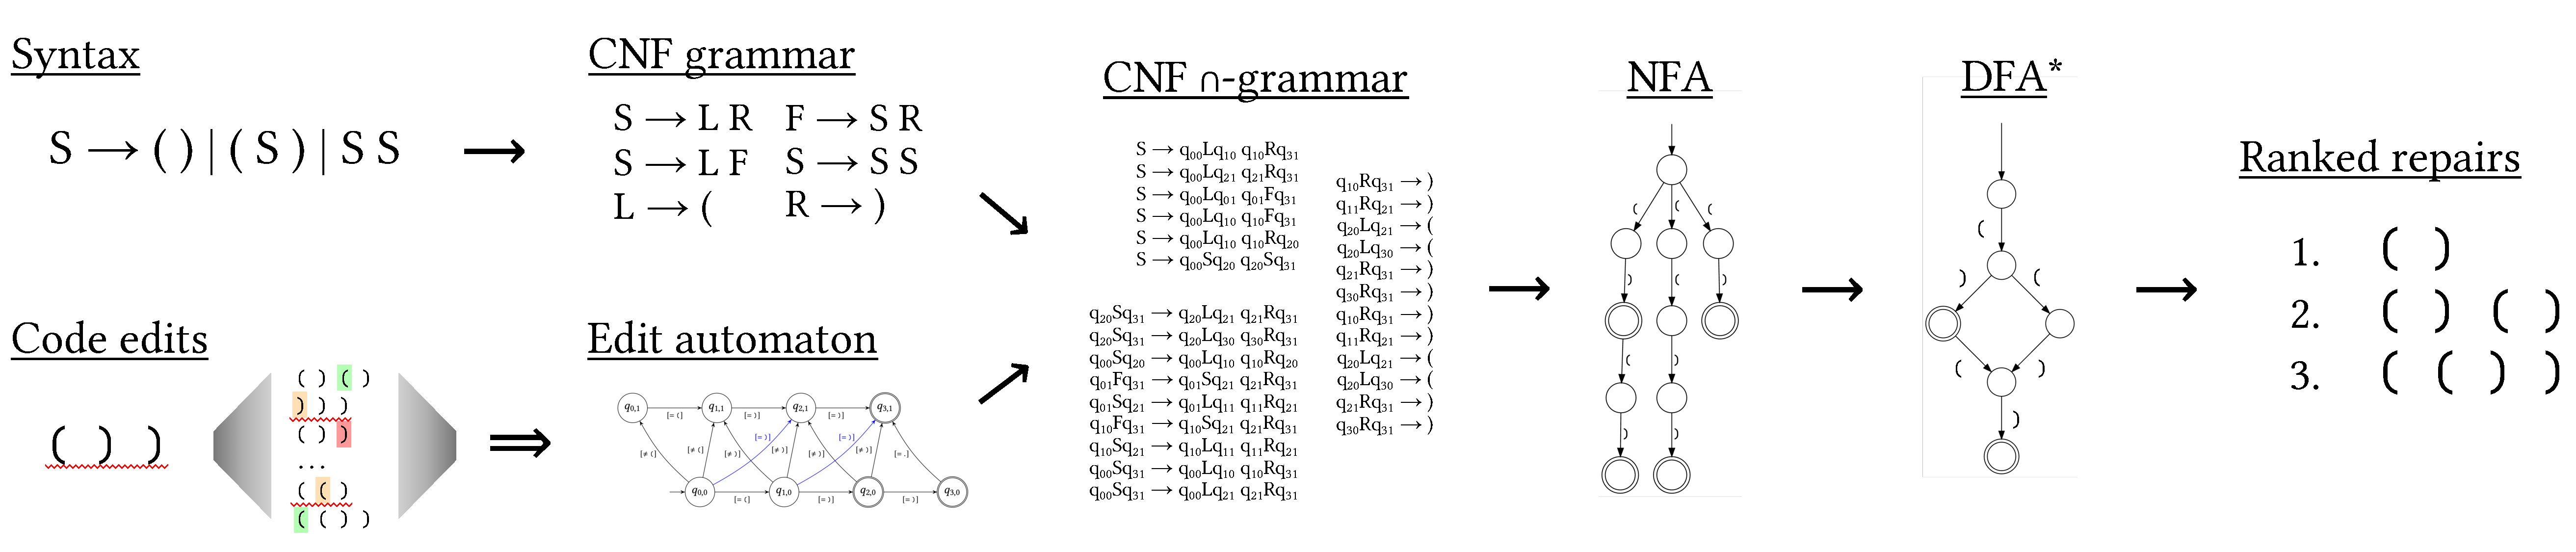
\includegraphics[width=\textwidth]{flow_short.pdf}
\vspace{0.1cm}
\caption{Simplified dataflow of the language intersection pipeline. Given a grammar and broken code fragment, we (1) create a automaton generating the language of small edits, then (2) construct a grammar representing the intersection of the two languages. This grammar can be (3) converted into a finite automaton, (4) determinized, then (5) decoded to produce a list of repairs.}
\label{fig:exampleDFA}
\end{figure}
\end{frame}

\section{Formal Language Theory}\label{sec:fltheory}

%------------------------------------------------------------------------------------------------

\begin{frame}[fragile]{Background: Regular grammars}
  A regular grammar (RG) is a quadruple $\mathcal{G} = \langle V, \Sigma, P, S\rangle$ where $V$ are nonterminals, $\Sigma$ are terminals, $P: V\times (V \cup \Sigma)^{\leq 2}$ are the productions, and $S\in V$ is the start symbol, i.e., all productions are of the form $A \rightarrow a$, $A \rightarrow a B$ (right-regular), or $A \rightarrow B a$ (left-regular). E.g., the following RG and NFA correspond to the language defined by the \textit{regex} \tinline{(a(ab)*)*(ba)*}:

  % https://www3.nd.edu/~kogge/courses/cse30151-fa17/Public/other/tikz_tutorial.pdf
  % Glushkov's algorithm: https://www.irif.fr/~jep/PDF/MPRI/MPRI.pdf#subsection.3.5.2
  \begin{figure}
    \hspace{-1cm}
    \begin{minipage}[t]{0.25\linewidth}
      \vspace{-2.4cm}\scalebox{0.6}{
        \begin{aligned}[t]
          S &\rightarrow Q_0 \mid Q_2 \mid Q_3 \mid Q_5\\
          Q_0 &\rightarrow \varepsilon \\
          Q_1 &\rightarrow Q_0 b \mid Q_2 b\\
          Q_2 &\rightarrow Q_1 a \\
          Q_3 &\rightarrow Q_0 a \mid Q_3 a \mid Q_5 a \\
          Q_4 &\rightarrow Q_3 a \mid Q_5 a \\
          Q_5 &\rightarrow Q_4 b \\
        \end{aligned}}
    \end{minipage}
    \hspace{0.5cm}
    \begin{minipage}[t]{0.48\linewidth}
      \scalebox{0.5}{
        \begin{tikzpicture}
          [->, >=stealth,]
          \node[state, initial above, accepting] (Q0) {$Q_0$};
          \node[state, left of=Q0] (Q1) {$Q_1$};
          \node[state, accepting, left of=Q1] (Q2) {$Q_2$};
          \node[state, accepting, right of=Q0] (Q3) {$Q_3$};
          \node[state, above right of=Q3] (Q4) {$Q_4$};
          \node[state, accepting, below right of=Q3] (Q5) {$Q_5$};
          \draw
          %        (Q0) edge[loop above] (Q0)
          (Q0) edge node{\ttinline b} (Q1)
          (Q0) edge node{\ttinline a} (Q3)
          (Q1) edge[bend right] node{\ttinline a} (Q2)
          (Q2) edge[bend right] node{\ttinline b} (Q1)
          (Q3) edge[loop above] node{\ttinline a} (Q3)
          (Q3) edge node{\ttinline a} (Q4)
          (Q5) edge node{\ttinline a} (Q3)
          (Q4) edge[bend left] node{\ttinline b} (Q5)
          (Q5) edge[bend left] node{\ttinline a} (Q4)
        \end{tikzpicture}
      }
    \end{minipage}
  \end{figure}

  \begin{center}
    \scalebox{0.8}{
      \begin{tikzpicture}[font=\sffamily,breathe dist/.initial=4ex]
        \foreach \X [count=\Y,remember=\Y as \LastY] in
          {finite,regular}
          {\ifnum\Y=1
        \node[ellipse,draw,outer sep=0pt] (F-\Y) {\X};
        \else
        \path[decoration={text along path,
        text={|\sffamily|\X},text align=center,raise=0.9ex},decorate]
        let \p1=($(F-\LastY.north)-(F-\LastY.west)$)
        in (F-\LastY.west) arc(180:0:\x1 and \y1);
        \path let \p1=($([yshift=\pgfkeysvalueof{/tikz/breathe dist}]F-\LastY.north)
        -(F-\LastY.south)$),
        \p2=($(F-1.east)-(F-1.west)$),\p3=($(F-1.north)-(F-1.south)$)
        in ($([yshift=\pgfkeysvalueof{/tikz/breathe dist}]F-\LastY.north)!0.5!(F-\LastY.south)$)
        node[minimum height=\y1,minimum width={\y1*\x2/\y3},
        draw,ellipse,inner sep=0pt, fill=black!30!white] (F-\Y){};
        \fi
        }
        \foreach \X [count=\Y,remember=\Y as \LastY] in
          {finite,regular,context-free}
          {\ifnum\Y=1
        \node[ellipse,draw,outer sep=0pt] (F-\Y) {\X};
        \else
        \path[decoration={text along path,
        text={|\sffamily|\X},text align=center,raise=0.9ex},decorate]
        let \p1=($(F-\LastY.north)-(F-\LastY.west)$)
        in (F-\LastY.west) arc(180:0:\x1 and \y1);
        \path let \p1=($([yshift=\pgfkeysvalueof{/tikz/breathe dist}]F-\LastY.north)
        -(F-\LastY.south)$),
        \p2=($(F-1.east)-(F-1.west)$),\p3=($(F-1.north)-(F-1.south)$)
        in ($([yshift=\pgfkeysvalueof{/tikz/breathe dist}]F-\LastY.north)!0.5!(F-\LastY.south)$)
        node[minimum height=\y1,minimum width={\y1*\x2/\y3},
        draw,ellipse,inner sep=0pt] (F-\Y){};
        \fi}
      \end{tikzpicture}
    }
  \end{center}
\end{frame}

    \begin{frame}[fragile]{Levenshtein automaton customization}

Consider the string $\err\sigma=$ \texttt{\scriptsize ( ) )} and the alphabet $\Sigma = \{\texttt{\scriptsize)}, \texttt{\scriptsize(}\}$. Every string within one edit of $\err\sigma$ is recognized by an NFA with the following structure:

\begin{figure}[h!]
\resizebox{0.45\textwidth}{!}{
\begin{tikzpicture}[
%->, % makes the edges directed
>=stealth',
node distance=2.5cm, % specifies the minimum distance between two nodes. Change if necessary.
%  every state/.style={thick, fill=gray!10}, % sets the properties for each ’state’ node
initial text=$ $, % sets the text that appears on the start arrow
]
\node[state, initial]                (00) {$q_{0,0}$};
\node[state, right of=00]            (10) {$q_{1,0}$};
\node[accepting, state, right of=10] (20) {$q_{2,0}$};
\node[accepting, state, right of=20] (30) {$q_{3,0}$};

\node[state, above of=00, shift={(-2cm,0cm)}] (01) {$q_{0,1}$};
\node[state, right of=01]                     (11) {$q_{1,1}$};
\node[state, right of=11]                     (21) {$q_{2,1}$};
\node[accepting, state, right of=21]          (31) {$q_{3,1}$};

\draw [->] (00) edge[below] node{$\texttt{(}$} (10);
\draw [->] (10) edge[below] node{$\texttt{)}$} (20);
\draw [->] (20) edge[below] node{$\texttt{)}$} (30);

\draw [->] (01) edge[below] node{$\texttt{(}$}                       (11);
\draw [->] (11) edge[below] node[shift={(-0.2cm,0cm)}]{$\texttt{)}$} (21);
\draw [->] (21) edge[below] node[shift={(-0.2cm,0cm)}]{$\texttt{)}$} (31);

\draw [->] (00) edge[bend left=10] node[shift={(-0.15cm,0cm)}]{\tiny{$\texttt{(}$}} (11);
\draw [->] (10) edge[bend left=10] node[shift={(-0.15cm,0cm)}]{\tiny{$\texttt{(}$}} (21);
\draw [->] (20) edge[bend left=10] node[shift={(-0.15cm,0cm)}]{\tiny{$\texttt{(}$}} (31);

\draw [->] (00) edge[bend left=10, left] node[shift={(-0.1cm,0cm)}]{\tiny{$\texttt{(}$}} (01);
\draw [->] (10) edge[bend left=10, left] node[shift={(-0.1cm,0cm)}]{\tiny{$\texttt{(}$}} (11);
\draw [->] (20) edge[bend left=10, left] node[shift={(-0.1cm,0cm)}]{\tiny{$\texttt{(}$}} (21);

\draw [->] (00) edge[bend right=10, right] node{\tiny{$\texttt{)}$}} (11);
\draw [->] (10) edge[bend right=10, right] node{\tiny{$\texttt{)}$}} (21);
\draw [->] (20) edge[bend right=10, right] node{\tiny{$\texttt{)}$}} (31);

\draw [->] (00) edge[bend right=10, right] node{\tiny{$\texttt{)}$}} (01);
\draw [->] (10) edge[bend right=10, right] node{\tiny{$\texttt{)}$}} (11);
\draw [->] (20) edge[bend right=10, right] node{\tiny{$\texttt{)}$}} (21);

\draw [->] (30) edge[bend left=10, left] node[shift={(-0.1cm,0cm)}]{\tiny{$\texttt{(}$}} (31);
\draw [->] (30) edge[bend right=10, right] node{\tiny{$\texttt{)}$}} (31);

\draw [->, blue] (00) edge[bend right=11,below] node[shift={(0.4cm,0.9cm)}]{$\texttt{)}$}    (21);
\draw [->, blue] (10) edge[bend right=11,below] node[shift={(0.4cm,0.9cm)}]{$\texttt{)}$}    (31);
\node[align=center, yshift=2em, xshift=-1cm] (title) at (current bounding box.north) {Original Levenshtein automaton};
\end{tikzpicture}
}
\resizebox{0.515\textwidth}{!}{
\begin{tikzpicture}[
%->, % makes the edges directed
>=stealth',
node distance=2.5cm, % specifies the minimum distance between two nodes. Change if necessary.
%  every state/.style={thick, fill=gray!10}, % sets the properties for each ’state’ node
initial text=$ $, % sets the text that appears on the start arrow
]
\draw[orange,->] (-4cm,1.2cm) -- (-3cm,1.2cm);

\node[state, initial]                (00) {$q_{0,0}$};
\node[state, right of=00]            (10) {$q_{1,0}$};
\node[accepting, state, right of=10] (20) {$q_{2,0}$};
\node[accepting, state, right of=20] (30) {$q_{3,0}$};

\node[state, above of=00, shift={(-2cm,0cm)}] (01) {$q_{0,1}$};
\node[state, right of=01]                     (11) {$q_{1,1}$};
\node[state, right of=11]                     (21) {$q_{2,1}$};
\node[accepting, state, right of=21]          (31) {$q_{3,1}$};

\draw [->] (00) edge[below] node{\tiny{$[= \texttt{(}]$}} (10);
\draw [->] (10) edge[below] node{\tiny{$[= \texttt{)}]$}} (20);
\draw [->] (20) edge[below] node{\tiny{$[= \texttt{)}]$}} (30);

\draw [->] (01) edge[below] node{\tiny{$[= \texttt{(}]$}}                       (11);
\draw [->] (11) edge[below] node[shift={(-0.2cm,0cm)}]{\tiny{$[= \texttt{)}]$}} (21);
\draw [->] (21) edge[below] node[shift={(-0.2cm,0cm)}]{\tiny{$[= \texttt{)}]$}} (31);

\draw [->] (00) edge[left] node{\tiny{$[\neq \texttt{(}]$}} (11);
\draw [->] (10) edge[left] node{\tiny{$[\neq \texttt{)}]$}} (21);
\draw [->] (20) edge[left] node{\tiny{$[\neq \texttt{)}]$}} (31);

\draw [->] (00) edge[bend left=10, left] node{\tiny{$[\neq \texttt{(}]$}} (01);
\draw [->] (10) edge[bend left=10, left] node{\tiny{$[\neq \texttt{)}]$}} (11);
\draw [->] (20) edge[bend left=10, left] node{\tiny{$[\neq \texttt{)}]$}} (21);
\draw [->] (30) edge[bend left=10, left] node{\tiny{$[=.]$}} (31);


\draw [->, blue] (00) edge[bend right=11,below] node[shift={(0.2cm,0.8cm)}]{\tiny{$[= \texttt{)}]$}}    (21);
\draw [->, blue] (10) edge[bend right=11,below] node[shift={(0.2cm,0.8cm)}]{\tiny{$[= \texttt{)}]$}}    (31);
\node[align=center, yshift=2em, xshift=-0.4cm] (title) at (current bounding box.north) {Nominal Levenshtein automaton (ours)};
\end{tikzpicture}
}
\caption{Automaton recognizing every single patch of the broken string \texttt{( ) )} within Levenshtein distance 1. We nominalize the original Levenshtein automaton, ensuring upward arcs denote a mutation, and replace terminals with a symbolic predicate, which deduplicates parallel arcs in large alphabets.}\label{fig:lev_automaton}\vspace{-5pt}
\end{figure}
\\
\tiny{\url{https://fulmicoton.com/posts/levenshtein/#observations-lets-count-states}}
\end{frame}

\begin{frame}[fragile]{Levenshtein reachability}
  \begin{figure}[H]
    \resizebox{\textwidth}{!}{
      \begin{tikzpicture}[
%->, % makes the edges directed
        >=stealth',
        node distance=2.5cm, % specifies the minimum distance between two nodes. Change if necessary.
%  every state/.style={thick, fill=gray!10}, % sets the properties for each ’state’ node
        initial text=$ $, % sets the text that appears on the start arrow
      ]
        \node[state, initial]                (00) {$q_{0,0}$};
        \node[state, right of=00]            (10) {$q_{1,0}$};
        \node[accepting, state, right of=10] (20) {$q_{2,0}$};
        \node[accepting, state, right of=20] (30) {$q_{3,0}$};
        \node[accepting, state, right of=30] (40) {$q_{4,0}$};
        \node[accepting, state, right of=40] (50) {$q_{5,0}$};

        \node[state, above of=00, shift={(-2cm,0cm)}] (01) {$q_{0,1}$};
        \node[state, right of=01]                          (11) {$q_{1,1}$};
        \node[state, right of=11]                          (21) {$q_{2,1}$};
        \node[accepting, state, right of=21]               (31) {$q_{3,1}$};
        \node[accepting, state, right of=31]               (41) {$q_{4,1}$};
        \node[accepting, state, right of=41]               (51) {$q_{5,1}$};

        \node[state, above of=01, shift={(-2cm,0cm)}] (0j) {$q_{0,2}$};
        \node[state, right of=0j]                          (1j) {$q_{1,2}$};
        \node[state, right of=1j]                          (2j) {$q_{2,2}$};
        \node[state, right of=2j]                          (3j) {$q_{3,2}$};
        \node[accepting, state, right of=3j]               (4j) {$q_{4,2}$};
        \node[accepting, state, right of=4j]               (5j) {$q_{5,2}$};

        \node[state, above of=0j, shift={(-2cm,0cm)}] (0k) {$q_{0,3}$};
        \node[state, right of=0k]                         (1k) {$q_{1,3}$};
        \node[state, right of=1k]                         (2k) {$q_{2,3}$};
        \node[state, right of=2k]                         (3k) {$q_{3,3}$};
        \node[state, right of=3k]                         (4k) {$q_{4,3}$};
        \node[accepting, state, right of=4k]              (5k) {$q_{5,3}$};

        \draw [->] (00) edge[below] node{$\sigma_1$} (10);
        \draw [->] (10) edge[below] node{$\sigma_2$} (20);
        \draw [->] (20) edge[below] node{$\sigma_3$} (30);
        \draw [->] (30) edge[below] node{$\sigma_4$} (40);
        \draw [->] (40) edge[below] node{$\sigma_5$} (50);

        \draw [->] (01) edge[below] node{$\sigma_1$} (11);
        \draw [->] (11) edge[below] node[shift={(-0.2cm,0cm)}]{$\sigma_2$} (21);
        \draw [->] (21) edge[below] node[shift={(-0.2cm,0cm)}]{$\sigma_3$} (31);
        \draw [->] (31) edge[below] node[shift={(-0.2cm,0cm)}]{$\sigma_4$} (41);
        \draw [->] (41) edge[below] node{$\sigma_5$} (51);

        \draw [->] (0j) edge[below] node{$\sigma_1$} (1j);
        \draw [->] (1j) edge[below] node{$\sigma_2$} (2j);
        \draw [->] (2j) edge[below] node{$\sigma_3$} (3j);
        \draw [->] (3j) edge[below] node{$\sigma_4$} (4j);
        \draw [->] (4j) edge[below] node{$\sigma_5$} (5j);

        \draw [->] (0k) edge[below] node{$\sigma_1$} (1k);
        \draw [->] (1k) edge[below] node{$\sigma_2$} (2k);
        \draw [->] (2k) edge[below] node{$\sigma_3$} (3k);
        \draw [->] (3k) edge[below] node{$\sigma_4$} (4k);
        \draw [->] (4k) edge[below] node{$\sigma_5$} (5k);

        \draw [->] (00) edge[left] node{$\phantom{\cdot}$} (11);
        \draw [->] (10) edge[left] node{$\phantom{\cdot}$} (21);
        \draw [->] (20) edge[left] node{$\phantom{\cdot}$} (31);
        \draw [->] (30) edge[left] node{$\phantom{\cdot}$} (41);
        \draw [->] (40) edge[left] node{$\phantom{\cdot}$} (51);

% Super-knight arcs
        \draw [->, red] (00) edge[bend right=8] node[east, shift={(-0.2cm,-0.7cm)}]{$\color{red}\sigma_3$}         (3j);
        \draw [->, red] (10) edge[bend right=8] node[east, shift={(-0.2cm,-0.7cm)}]{$\color{red}\sigma_4$}         (4j);
        \draw [->, red] (20) edge[bend right=8] node[east, shift={(-0.2cm,-0.7cm)}]{$\color{red}\sigma_5$}         (5j);

        \draw [->, red] (01) edge[bend left=8] node[east, shift={(-0.2cm,-0.7cm)}]{$\color{red}\sigma_3$}         (3k);
        \draw [->, red] (11) edge[bend left=8] node[east, shift={(-0.2cm,-0.7cm)}]{$\color{red}\sigma_4$}         (4k);
        \draw [->, red] (21) edge[bend left=8] node[east, shift={(-0.2cm,-0.7cm)}]{$\color{red}\sigma_5$}         (5k);

        \draw [->, violet] (00) edge node[east, shift={(-0.1cm,-0.8cm)}]{$\color{violet}\sigma_4$}  (4k);
        \draw [->, violet] (10) edge node[east, shift={(-0.1cm,-0.8cm)}]{$\color{violet}\sigma_5$}  (5k);

        \draw [->] (01) edge[left] node{$\phantom{\cdot}$} (1j);
        \draw [->] (11) edge[left] node{$\phantom{\cdot}$} (2j);
        \draw [->] (21) edge[left] node{$\phantom{\cdot}$} (3j);
        \draw [->] (31) edge[left] node{$\phantom{\cdot}$} (4j);
        \draw [->] (41) edge[left] node{$\phantom{\cdot}$} (5j);

        \draw [->] (0j) edge[left] node{$\phantom{\cdot}$} (1k);
        \draw [->] (1j) edge[left] node{$\phantom{\cdot}$} (2k);
        \draw [->] (2j) edge[left] node{$\phantom{\cdot}$} (3k);
        \draw [->] (3j) edge[left] node{$\phantom{\cdot}$} (4k);
        \draw [->] (4j) edge[left] node{$\phantom{\cdot}$} (5k);

        \draw [->] (00) edge[bend left=10, left] node{$\phantom{\cdot}$} (01);
        \draw [->] (10) edge[bend left=10, left] node{$\phantom{\cdot}$} (11);
        \draw [->] (20) edge[bend left=10, left] node{$\phantom{\cdot}$} (21);
        \draw [->] (30) edge[bend left=10, left] node{$\phantom{\cdot}$} (31);
        \draw [->] (40) edge[bend left=10, left] node{$\phantom{\cdot}$} (41);
        \draw [->] (50) edge[bend left=10, left] node{$\phantom{\cdot}$} (51);

        \draw [->] (01) edge[bend left=10, left] node{$\phantom{\cdot}$} (0j);
        \draw [->] (11) edge[bend left=10, left] node{$\phantom{\cdot}$} (1j);
        \draw [->] (21) edge[bend left=10, left] node{$\phantom{\cdot}$} (2j);
        \draw [->] (31) edge[bend left=10, left] node{$\phantom{\cdot}$} (3j);
        \draw [->] (41) edge[bend left=10, left] node{$\phantom{\cdot}$} (4j);
        \draw [->] (51) edge[bend left=10, left] node{$\phantom{\cdot}$} (5j);

        \draw [->] (0j) edge[bend left=10, left] node{$\phantom{\cdot}$} (0k);
        \draw [->] (1j) edge[bend left=10, left] node{$\phantom{\cdot}$} (1k);
        \draw [->] (2j) edge[bend left=10, left] node{$\phantom{\cdot}$} (2k);
        \draw [->] (3j) edge[bend left=10, left] node{$\phantom{\cdot}$} (3k);
        \draw [->] (4j) edge[bend left=10, left] node{$\phantom{\cdot}$} (4k);
        \draw [->] (5j) edge[bend left=10, left] node{$\phantom{\cdot}$} (5k);

        \draw [->, blue] (00) edge[bend right=11,below] node[shift={(0.5cm,0.3cm)}]{$\color{blue}\sigma_2$}    (21);
        \draw [->, blue] (10) edge[bend right=11,below] node[shift={(0.5cm,0.3cm)}]{$\color{blue}\sigma_3$}    (31);
        \draw [->, blue] (20) edge[bend right=11,below] node[shift={(0.5cm,0.3cm)}]{$\color{blue}\sigma_4$}    (41);
        \draw [->, blue] (30) edge[bend right=11,below] node[shift={(0.5cm,0.3cm)}]{$\color{blue}\sigma_5$}    (51);

        \draw [->, blue] (01) edge[bend right=3,below] node[shift={(0.3cm,0.2cm)}]{$\color{blue}\sigma_2$}    (2j);
        \draw [->, blue] (11) edge[bend right=3,below] node[shift={(0.3cm,0.2cm)}]{$\color{blue}\sigma_3$}    (3j);
        \draw [->, blue] (21) edge[bend right=3,below] node[shift={(0.3cm,0.2cm)}]{$\color{blue}\sigma_4$}    (4j);
        \draw [->, blue] (31) edge[bend right=3,below] node[shift={(0.3cm,0.2cm)}]{$\color{blue}\sigma_4$}    (5j);

        \draw [->, blue] (0j) edge[bend left=8,below] node[shift={(-0.45cm,-0.55cm)}]{$\color{blue}\sigma_2$}    (2k);
        \draw [->, blue] (1j) edge[bend left=8,below] node[shift={(-0.45cm,-0.55cm)}]{$\color{blue}\sigma_3$}    (3k);
        \draw [->, blue] (2j) edge[bend left=8,below] node[shift={(-0.45cm,-0.55cm)}]{$\color{blue}\sigma_4$}    (4k);
        \draw [->, blue] (3j) edge[bend left=8,below] node[shift={(-0.45cm,-0.55cm)}]{$\color{blue}\sigma_5$}    (5k);

%https://tex.stackexchange.com/a/20986/139648
        \draw [decorate,decoration={brace,amplitude=10pt,raise=10pt,mirror}] (00.south west) -- (50.south east) node[midway,yshift=-3em]{\textbf{String length}};
        \draw [decorate,decoration={brace,amplitude=10pt,raise=20pt}] (00.south west) -- (0k.north west) node[midway,xshift=-1cm,yshift=-1cm,rotate=-54]{\textbf{Edit distance}};
      \end{tikzpicture}
    }
    \caption{Bounded Levenshtein reachability from $\sigma: \Sigma^n$ is expressible as an NFA populated by accept states within radius $k$ of $S=q_{n,0}$, which accepts all strings $\sigma'$ within Levenshtein radius $k$ of $\sigma$.}
  \end{figure}
\end{frame}

\begin{frame}[fragile]{Geometrically interpreting the edit calculus}

Each arc plays a specific role. $\duparrow$ handles insertions, $\ddiagarrow$ handles substitutions and $\knightarrow$ handles deletions of $\geq 1$ tokens. Consider some illustrative cases:

\vspace{0.5cm}

\newcommand{\substitutionExample}{
\tikz{
\foreach \x in {0,8,16,24,32,40}{
\fill (\x pt,0pt) circle [radius = 1pt];
\fill (\x pt,8pt) circle [radius = 1pt];
}
\phantom{\fill (0pt,-8pt) circle [radius = 1pt];}
\draw [-to] (0pt,0pt) -- (8pt,0pt);
\draw [-to] (8pt,0pt) -- (16pt,0pt);
\draw [-to] (16pt,0pt) -- (24pt,8pt);
\draw [-to] (24pt,8pt) -- (32pt,8pt);
\draw [-to] (32pt,8pt) -- (40pt,8pt);
}
}

\newcommand{\insertionExample}{
\tikz{
\foreach \x in {0,8,16,24,32,40}{
\fill (\x pt,0pt) circle [radius = 1pt];
\fill (\x pt,8pt) circle [radius = 1pt];
}
\phantom{\fill (0pt,-8pt) circle [radius = 1pt];}
\fill[white] (16pt,0pt) circle [radius = 1.2pt];
\fill[white] (24pt,8pt) circle [radius = 1.2pt];
\draw [-to] (0pt,0pt) -- (8pt,0pt);
\draw [-to] (8pt,0pt) -- (24pt,0pt);
\draw [-to] (24pt,0pt) -- (16pt,8pt);
\draw [-to] (16pt,8pt) -- (32pt,8pt);
\draw [-to] (32pt,8pt) -- (40pt,8pt);
}
}

\newcommand{\deletionExample}{
\tikz{
\foreach \x in {0,8,16,24,32,40}{
\fill (\x pt,0pt) circle [radius = 1pt];
\fill (\x pt,8pt) circle [radius = 1pt];
}
\phantom{\fill (0pt,-8pt) circle [radius = 1pt];}
\draw [-to] (0pt,0pt) -- (8pt,0pt);
\draw [-to] (8pt,0pt) -- (16pt,0pt);
\draw [-to] (16pt,0pt) -- (24pt,0pt);
\draw [-to] (24pt,0pt) -- (40pt,8pt);
}
}

\newcommand{\doubleDeletionExample}{
\tikz{
\foreach \x in {0,8,16,24,32,40}{
\fill (\x pt,0pt) circle [radius = 1pt];
\fill (\x pt,8pt) circle [radius = 1pt];
\fill (\x pt,16pt) circle [radius = 1pt];
}
\draw [-to] (0pt,0pt) -- (24pt,16pt);
\draw [-to] (24pt,16pt) -- (32pt,16pt);
\draw [-to] (32pt,16pt) -- (40pt,16pt);
}
}

\newcommand{\subDelExample}{
\tikz{
\foreach \x in {0,8,16,24,32,40}{
\fill (\x pt,0pt) circle [radius = 1pt];
\fill (\x pt,8pt) circle [radius = 1pt];
\fill (\x pt,16pt) circle [radius = 1pt];
}
\draw [-to] (0pt,0pt) -- (8pt,0pt);
\draw [-to] (8pt,0pt) -- (16pt,8pt);
\draw [-to] (16pt,8pt) -- (32pt,16pt);
\draw [-to] (32pt,16pt) -- (40pt,16pt);
}
}

\newcommand{\subSubExample}{
\tikz{
\foreach \x in {0,8,16,24,32,40}{
\fill (\x pt,0pt) circle [radius = 1pt];
\fill (\x pt,8pt) circle [radius = 1pt];
\fill (\x pt,16pt) circle [radius = 1pt];
}
\draw [-to] (0pt,0pt) -- (8pt,0pt);
\draw [-to] (8pt,0pt) -- (16pt,8pt);
\draw [-to] (16pt,8pt) -- (24pt,16pt);
\draw [-to] (24pt,16pt) -- (32pt,16pt);
\draw [-to] (32pt,16pt) -- (40pt,16pt);
}
}

\newcommand{\insertDeleteExample}{
\tikz{
\foreach \x in {0,8,16,24,32,40,48}{
\fill (\x pt,0pt) circle [radius = 1pt];
\fill (\x pt,8pt) circle [radius = 1pt];
\fill (\x pt,16pt) circle [radius = 1pt];
}
\fill[white] (16pt,16pt) circle [radius = 1.2pt];
\fill[white] (8pt,0pt) circle [radius = 1.2pt];
\fill[white] (16pt,8pt) circle [radius = 1.2pt];
\draw [-to] (0pt,0pt) -- (16pt,0pt);
\draw [-to] (16pt,0pt) -- (8pt,8pt);
\draw [-to] (8pt,8pt) -- (24pt,8pt);
\draw [-to] (24pt,8pt) -- (40pt,16pt);
\draw [-to] (40pt,16pt) -- (48pt,16pt);
}
}

\footnotesize{
\begin{table}[h!]
\begin{tabular}{ccccc}

\texttt{f\hspace{3pt}.\hspace{3pt}\hlorange{[}\hspace{3pt}x\hspace{3pt})} &
\texttt{f\hspace{3pt}.\hspace{3pt}\phantom{(}\hspace{3pt}x\hspace{3pt})} &
\texttt{f\hspace{3pt}.\hspace{3pt}(\hspace{3pt}\hlred{x}\hspace{3pt})} &
\texttt{\hlred{.}\hspace{3pt}\hlred{+}\hspace{3pt}(\hspace{3pt}x\hspace{3pt})} &
\texttt{f\hspace{3pt}\hlorange{.}\hspace{3pt}\hlred{(}\hspace{3pt}x\hspace{3pt};} \\

\texttt{f\hspace{3pt}.\hspace{3pt}\hlorange{(}\hspace{3pt}x\hspace{3pt})} &
\texttt{f\hspace{3pt}.\hspace{3pt}\hlgreen{(}\hspace{3pt}x\hspace{3pt})} &
\texttt{f\hspace{3pt}.\hspace{3pt}(\hspace{3pt}\phantom{x}\hspace{3pt})} &
\texttt{\phantom{f}\hspace{3pt}\phantom{.}\hspace{3pt}(\hspace{3pt}x\hspace{3pt})} &
\texttt{f\hspace{3pt}\hlorange{*}\hspace{3pt}\phantom{(}\hspace{3pt}x\hspace{3pt};} \\

\substitutionExample & \insertionExample & \deletionExample & \doubleDeletionExample & \subDelExample
\end{tabular}
\end{table}
}

\normalsize{Note that the same $\langle\err\sigma, \sigma'\rangle$ pair can have multiple Levenshtein alignments:}
\vspace{0.5cm}

\footnotesize{
\begin{table}[h!]
\begin{tabular}{cc}

\texttt{[\hspace{3pt}\hlorange{,}\hspace{3pt}\hlorange{x}\hspace{3pt}y\hspace{3pt}]} &
\texttt{[\hspace{3pt}\phantom{,}\hspace{3pt},\hspace{3pt}\hlred{x}\hspace{3pt}y\hspace{3pt}]} \\

\texttt{[\hspace{3pt}\hlorange{x}\hspace{3pt}\hlorange{,}\hspace{3pt}y\hspace{3pt}]} &
\texttt{[\hspace{3pt}\hlgreen{x}\hspace{3pt},\hspace{3pt}\phantom{x}\hspace{3pt}y\hspace{3pt}]} \\

\subSubExample & \insertDeleteExample
\end{tabular}
\end{table}
}

\normalsize{Non-uniqueness of geodesics has implications for CFG $\cap$ L-NFA ambiguity.}
\end{frame}

\begin{frame}[fragile]{The nominal Levenshtein automaton}
  The original Levenshtein automaton (Schulz \& Stoyan, 2002):

  \begin{prooftree}
    \AxiomC{$s\in\Sigma \phantom{\land} i \in [0, n] \phantom{\land} j \in [1, k]$}
    \RightLabel{$\duparrow$}
    \UnaryInfC{$(q_{i, j-1} \overset{s}{\rightarrow} q_{i,j}) \in \delta$}
    \DisplayProof
    \hskip 1.5em
    \AxiomC{$s\in\Sigma \phantom{\land} i \in [1, n] \phantom{\land} j \in [1, k]$}
    \RightLabel{$\ddiagarrow$}
    \UnaryInfC{$(q_{i-1, j-1} \overset{s}{\rightarrow} q_{i,j}) \in \delta$}
  \end{prooftree}
  \begin{prooftree}
    \AxiomC{$s=\sigma_i \phantom{\land} i \in [1, n] \phantom{\land} j \in [0, k]$}
    \RightLabel{$\drightarrow$}
    \UnaryInfC{$(q_{i-1, j} \overset{s}{\rightarrow} q_{i,j}) \in \delta$}
    \DisplayProof
    \hskip 1.5em
    \AxiomC{$s=\sigma_i \phantom{\land} i \in [2, n] \phantom{\land} j \in [1, k]$}
    \RightLabel{$\knightarrow$}
    \UnaryInfC{$(q_{i-2, j-1} \overset{s}{\rightarrow} q_{i,j}) \in \delta$}
  \end{prooftree}
  \begin{prooftree}
    \AxiomC{$\vphantom{|}$}
    \RightLabel{$\textsc{Init}$}
    \UnaryInfC{$q_{0,0} \in I$}
    \DisplayProof
    \hskip 1.5em
    \AxiomC{$q_{i, j}$}
    \AxiomC{$|n-i+j| \leq k$}
    \RightLabel{$\textsc{Done}$}
    \BinaryInfC{$q_{i, j}\in F$}
  \end{prooftree}

  We modify the original automaton with a nominal predicate:

  \begin{prooftree}
    \AxiomC{$i \in [0, n] \phantom{\land} j \in [1, k]$}
    \RightLabel{$\duparrow$}
    \UnaryInfC{$(q_{i, j-1} \overset{{\color{orange}[\neq \sigma_{i+1}]}}{\rightarrow} q_{i,j}) \in \delta$}
    \DisplayProof
    \hskip 1.5em
    \AxiomC{$i \in [1, n] \phantom{\land} j \in [1, k]$}
    \RightLabel{$\ddiagarrow$}
    \UnaryInfC{$(q_{i-1, j-1} \overset{{\color{orange}[\neq \sigma_i]}}{\rightarrow} q_{i,j}) \in \delta$}
  \end{prooftree}
  \begin{prooftree}
    \AxiomC{$i \in [1, n] \phantom{\land} j \in [0, k]$}
    \RightLabel{$\drightarrow$}
    \UnaryInfC{$(q_{i-1, j} \overset{{\color{orange}[=\sigma_i]}}{\rightarrow} q_{i,j}) \in \delta$}
    \DisplayProof
    \hskip 1.5em
    \AxiomC{$d \in [1, d_{\max}] \phantom{\land} i \in [d + 1, n] \phantom{\land} j \in [d, k]$}
    \RightLabel{$\knightarrow$}
    \UnaryInfC{$(q_{i-d-1, j-d} \overset{{\color{orange}[=\sigma_i]}}{\rightarrow} q_{i,j}) \in \delta$}
  \end{prooftree}
\end{frame}

\begin{frame}{Background: Context-free grammars}
  In a context-free grammar $\mathcal{G} = \langle V, \Sigma, P, S\rangle$ all productions are of the form $P: V\times (V \cup \Sigma)^+$, i.e., RHS may contain any number of nonterminals, $V$. Recognition decidable in $\mathcal{O}(n^\omega)$, n.b. CFLs are \textbf{not} closed under $\cap$!\newline\\
  %
  For example, consider the grammar $\underline{S \rightarrow S S \mid ( S ) \mid ()}$. This represents the language of balanced parentheses, e.g. $(), ()(), (()), ()(()), (()()), (())()\ldots$\newline\\
  %
  Every CFG has a normal form $P^*: V \times (V^2 \mid \Sigma)$, i.e., every production can be refactored into either $v_0 \rightarrow v_1 v_2$ or $v_0 \rightarrow \sigma$, where $v_{0\ldots2}: V$ and $\sigma: \Sigma$, e.g., $\{S \rightarrow S S \mid ( S ) \mid ()\}\Leftrightarrow^*\{S\rightarrow XR \mid SS \mid LR, L \rightarrow (, R \rightarrow ), X\rightarrow LS\}$

  \begin{center}
    \scalebox{0.8}{
      \begin{tikzpicture}[font=\sffamily,breathe dist/.initial=4ex]
        \foreach \X [count=\Y,remember=\Y as \LastY] in
          {finite,regular,context-free}
          {\ifnum\Y=1
        \node[ellipse,draw,outer sep=0pt] (F-\Y) {\X};
        \else
        \path[decoration={text along path,
        text={|\sffamily|\X},text align=center,raise=0.9ex},decorate]
        let \p1=($(F-\LastY.north)-(F-\LastY.west)$)
        in (F-\LastY.west) arc(180:0:\x1 and \y1);
        \path let \p1=($([yshift=\pgfkeysvalueof{/tikz/breathe dist}]F-\LastY.north)
        -(F-\LastY.south)$),
        \p2=($(F-1.east)-(F-1.west)$),\p3=($(F-1.north)-(F-1.south)$)
        in ($([yshift=\pgfkeysvalueof{/tikz/breathe dist}]F-\LastY.north)!0.5!(F-\LastY.south)$)
        node[minimum height=\y1,minimum width={\y1*\x2/\y3},
        draw,ellipse,inner sep=0pt, fill=black!30!white] (F-\Y){};
        \fi
        }
        \foreach \X [count=\Y,remember=\Y as \LastY] in
          {finite,regular,context-free,conjunctive}
          {\ifnum\Y=1
        \node[ellipse,draw,outer sep=0pt] (F-\Y) {\X};
        \else
        \path[decoration={text along path,
        text={|\sffamily|\X},text align=center,raise=0.9ex},decorate]
        let \p1=($(F-\LastY.north)-(F-\LastY.west)$)
        in (F-\LastY.west) arc(180:0:\x1 and \y1);
        \path let \p1=($([yshift=\pgfkeysvalueof{/tikz/breathe dist}]F-\LastY.north)
        -(F-\LastY.south)$),
        \p2=($(F-1.east)-(F-1.west)$),\p3=($(F-1.north)-(F-1.south)$)
        in ($([yshift=\pgfkeysvalueof{/tikz/breathe dist}]F-\LastY.north)!0.5!(F-\LastY.south)$)
        node[minimum height=\y1,minimum width={\y1*\x2/\y3},
        draw,ellipse,inner sep=0pt] (F-\Y){};
        \fi}
      \end{tikzpicture}
    }
  \end{center}
\end{frame}

\begin{frame}{Background: CFGs as substructural logics}
  CFGs can also be viewed as a very weak substructural logic. The logic has no type constructor and the only inference rule is \textsc{Cut}. The goal of parsing is, given some string $\sigma: \Sigma^n$, to prove $\sigma \vdash [S, 0, n]$.

\vspace{0.5cm}

\begin{figure}
\begin{prooftree}
\AxiomC{$(W\rightarrow\sigma_i) \in P$}
\RightLabel{\textsc{Int}}
\UnaryInfC{$[W, i, i+1]$}
\DisplayProof
\hskip 1.5em
\AxiomC{$(W \rightarrow X Z) \in P$}
\AxiomC{$[X, i, j]$}
\AxiomC{$[Z, j, k]$}
\RightLabel{\textsc{Cut}}
\TrinaryInfC{$[W, i, k]$}
\end{prooftree}
\caption{Context-free parsing as a substructural logic.}
\end{figure}

  This logic can be enriched by considering categorial grammars, which associates to each nonterminal a set of types, however the resulting expressivity is (mostly) unchanged, as proven by Pentus in 1991. Lambek argues the equivalent CFG is typically less comprehensible in practice.
 % https://www.math.mcgill.ca/barr/lambek/pdffiles/logicandgr.pdf
 % https://www.math.mcgill.ca/barr/papers/pga.pdf#page=53
 % https://www.math.mcgill.ca/barr/papers/pga.pdf#page=65
 % https://festschriften.illc.uva.nl/j50/contribs/kanazawa/kanazawa.pdf
 % https://arxiv.org/pdf/2405.16662#page=4
 % http://www.eecs.harvard.edu/~shieber/Biblio/Papers/infer.pdf
\end{frame}

%\begin{frame}{Background: Conjunctive grammars}
%  Conjunctive grammars naturally extend CFGs with CFL union and intersection, respecting closure under those operations. Equivalent to trellis automata, which are like contractive elementary cellular automata. Language inclusion is decidable in P.\\
%
%  \begin{prooftree}
%    \AxiomC{$\Gamma \vdash \mathcal{G}_1, \mathcal{G}_2 : \texttt{CG}$}
%    \RightLabel{$\cap$}
%    \UnaryInfC{$\Gamma \vdash \exists \:\mathcal{G}_3: \texttt{CG}\:.\:\mathcal{L}_{\mathcal{G}_1} \cap \mathcal{L}_{\mathcal{G}_1} \leftrightarrow \mathcal{G}_3$}
%  \end{prooftree}
%
%  \begin{center}
%    \scalebox{0.8}{
%      \begin{tikzpicture}[font=\sffamily,breathe dist/.initial=4ex]
%        \foreach \X [count=\Y,remember=\Y as \LastY] in
%          {finite,regular,context-free,conjunctive}
%          {\ifnum\Y=1
%        \node[ellipse,draw,outer sep=0pt] (F-\Y) {\X};
%        \else
%        \path[decoration={text along path,
%        text={|\sffamily|\X},text align=center,raise=0.9ex},decorate]
%        let \p1=($(F-\LastY.north)-(F-\LastY.west)$)
%        in (F-\LastY.west) arc(180:0:\x1 and \y1);
%        \path let \p1=($([yshift=\pgfkeysvalueof{/tikz/breathe dist}]F-\LastY.north)
%        -(F-\LastY.south)$),
%        \p2=($(F-1.east)-(F-1.west)$),\p3=($(F-1.north)-(F-1.south)$)
%        in ($([yshift=\pgfkeysvalueof{/tikz/breathe dist}]F-\LastY.north)!0.5!(F-\LastY.south)$)
%        node[minimum height=\y1,minimum width={\y1*\x2/\y3},
%        draw,ellipse,inner sep=0pt, fill=black!30!white] (F-\Y){};
%        \fi
%        }
%        \foreach \X [count=\Y,remember=\Y as \LastY] in
%          {finite,regular,context-free,conjunctive,context sensitive}
%          {\ifnum\Y=1
%        \node[ellipse,draw,outer sep=0pt] (F-\Y) {\X};
%        \else
%        \path[decoration={text along path,
%        text={|\sffamily|\X},text align=center,raise=0.9ex},decorate]
%        let \p1=($(F-\LastY.north)-(F-\LastY.west)$)
%        in (F-\LastY.west) arc(180:0:\x1 and \y1);
%        \path let \p1=($([yshift=\pgfkeysvalueof{/tikz/breathe dist}]F-\LastY.north)
%        -(F-\LastY.south)$),
%        \p2=($(F-1.east)-(F-1.west)$),\p3=($(F-1.north)-(F-1.south)$)
%        in ($([yshift=\pgfkeysvalueof{/tikz/breathe dist}]F-\LastY.north)!0.5!(F-\LastY.south)$)
%        node[minimum height=\y1,minimum width={\y1*\x2/\y3},
%        draw,ellipse,inner sep=0pt] (F-\Y){};
%        \fi}
%      \end{tikzpicture}
%    }
%  \end{center}
%\end{frame}


\begin{frame}[fragile]{Background: Closure properties of formal languages}
  Formal languages are not always closed under set-theoretic operations, e.g., CFL $\cap$ CFL is not CFL in general. Let $\cdot$ denote concatenation, $*$ be Kleene star, and $\complement$ be complementation:\\
  \begin{table}
    \begin{tabular}{c|ccccc}
      & $\cup$ & $\cap$ & $\cdot$ & $*$ & $\complement$ \\\hline
      Finite$^1$                                  & \cmark & \cmark     & \cmark  & \cmark  & \cmark \\
      Regular$^1$                                 & \cmark & \cmark     & \cmark  & \cmark  & \cmark \\
      \rowcolor{slightgray} Context-free$^{1, 2}$ & \cmark & \xmark$^\dagger$ & \cmark  & \cmark  & \xmark \\
      Conjunctive$^{1,2}$                         & \cmark & \cmark     & \cmark  & \cmark  & ?      \\
      Context-sensitive$^2$                       & \cmark & \cmark     & \cmark  & +       & \cmark \\
      Recursively Enumerable$^2$                  & \cmark & \cmark     & \cmark  & \cmark  & \xmark \\
    \end{tabular}
  \end{table}
  We would like a language family that is (1) tractable, i.e., has polynomial recognition and search complexity and (2) reasonably expressive, i.e., can represent syntactic properties of real-world programming languages.\vspace{0.2cm}

  $^\dagger$ However, CFLs are closed under intersection with regular languages.
\end{frame}

\begin{frame}[fragile]{The Bar-Hillel construction and its specialization}
  The original Bar-Hillel construction provides a way to construct a grammar for the intersection of a regular and context-free language.
  \noindent\begin{prooftree}
    \AxiomC{$q \in I \phantom{\land} r \in F\vphantom{\overset{a}{\rightarrow}}$}
    \RightLabel{$\sqrt{\phantom{S}}$}
    \UnaryInfC{$\big(S\rightarrow q S r\big) \in P_\cap$}
    \DisplayProof
    \hskip 2em
    \AxiomC{$(A \rightarrow a) \in P$}
    \AxiomC{$(q\overset{a}{\rightarrow}r) \in \delta$}
    \RightLabel{$\uparrow$}
    \BinaryInfC{$\big(qAr\rightarrow a\big)\in P_\cap$}
    \DisplayProof
    \AxiomC{$(w \rightarrow xz) \in P\vphantom{\overset{a}{\rightarrow}}$}
    \AxiomC{$p,q,r \in Q$}
    \RightLabel{$\Join$}
    \BinaryInfC{$\big(pwr\rightarrow (pxq)(qzr)\big) \in P_\cap$}
  \end{prooftree}

  We specialize the Bar-Hillel construction to nominal Levenshtein automata:

  \begin{prooftree}
    \AxiomC{$(A \rightarrow a) \in P$}
    \AxiomC{$(q\overset{{\color{orange}[\cdot]}}{\rightarrow}r) \in \delta$}
    \AxiomC{$\color{orange}a[\cdot]$}
    \RightLabel{$\hat\uparrow$}
    \TrinaryInfC{$\big(qAr\rightarrow a\big)\in P_\cap$}
    \DisplayProof
    \AxiomC{$\vphantom{\overset{[\cdot]}{\rightarrow}}\color{orange} w \triangleleft pr \phantom{\land} x \triangleleft pq \phantom{\land} z \triangleleft qr$}
    \AxiomC{$(w \rightarrow xz) \in P\vphantom{\overset{a}{\rightarrow}}$}
    \AxiomC{$p,q,r \in Q$}
    \RightLabel{$\hat\Join$}
    \TrinaryInfC{$\big(pwr\rightarrow (pxq)(qzr)\big) \in P_\cap$}
  \end{prooftree}

  Where $\triangleleft$ denotes compatibility between the Parikh map of a nonterminal and Levenshtein margin between two NFA states, see our paper for details.
\end{frame}

\section{Algebraic Parsing}\label{sec:algebraic-parsing}

\begin{frame}[fragile]{Parsing for linear algebraists}
  Given a CFG $\mathcal{G} \coloneqq \langle V, \Sigma, P, S\rangle$ in Chomsky Normal Form, we can construct a recognizer $R_\mathcal{G}: \Sigma^n \rightarrow \mathbb{B}$ for strings $\sigma: \Sigma^n$ as follows. Let $2^V$ be our domain, $0$ be $\varnothing$, $\oplus$ be $\cup$, and $\otimes$ be defined as follows:

  \vspace{-7pt}
  \[
    s_1 \otimes s_2 \coloneqq \{C \mid \langle A, B\rangle \in s_1 \times s_2, (C\rightarrow AB) \in P\}\\
    \text{e.g.},
    \{A \rightarrow BC, C \rightarrow AD, D \rightarrow BA\} \subseteq P \vdash \{A, B, C\} \otimes \{B, C, D\} = \{A, C\}
  \]
  \vspace{-1.5cm}

  \noindent If we define $\sigma_r^{\shur} \coloneqq \{w \mid (w \rightarrow \sigma_r) \in P\}$, then initialize $M^0_{r+1=c}(\mathcal{G}', e) := \;\sigma_r^{\shur}$ and solve for the fixpoint $M^* = M + M^2$,\vspace{-10pt}

  \begin{align*}
    M^0:=
    \begin{pNiceMatrix}[xdots/line-style=loosely dotted]
      \varnothing & \sigma_1^\shri & \varnothing & \Cdots & \varnothing \\
      \Vdots      & \Ddots         & \Ddots      & \Ddots & \Vdots\\
                  &                &             &        & \varnothing\\
                  &                &             &        & \sigma_n^\shup \\
      \varnothing & \Cdots         &             &        & \varnothing
    \end{pNiceMatrix} &\Rightarrow \ldots \Rightarrow M^* =
    \begin{pNiceMatrix}[xdots/line-style=loosely dotted]
      \varnothing & \sigma_1^\shri & \Lambda & \Cdots & \Lambda^*_\sigma\\
      \Vdots      & \Ddots         & \Ddots  & \Ddots & \Vdots\\
                  &                &         &        & \Lambda\\
                  &                &         &        & \sigma_n^\shup \\
      \varnothing & \Cdots         &         &        & \varnothing
    \end{pNiceMatrix}
  \end{align*}

  \noindent $S \Rightarrow^* \sigma \iff \sigma \in \mathcal{L}(\mathcal{G})$ iff $S \in \Lambda^*_\sigma$, i.e., $\mathds{1}_{\Lambda^*_\sigma}(S) \iff \mathds{1}_{\mathcal{L}(\mathcal{G})}(\sigma)$.
\end{frame}

\begin{frame}[fragile]{Lattices, Matrices and Trellises}
  The art of treillage has been practiced from ancient through modern times.
  \begin{center}
    \begin{tabular}{ c c c c c }
      \includegraphics[width=0.17\textwidth]{../figures/trellis.png} & & \includegraphics[width=0.12\textwidth]{../figures/grid_topiary.jpeg} & & \includegraphics[width=0.23\textwidth]{../figures/tree_pyramid.jpeg} \\\\
      \includegraphics[width=0.17\textwidth]{../figures/jiaxian_triangle.png} & &
      \rotatebox{37}{\scalebox{0.9}{$
      \begin{pNiceMatrix}[nullify-dots,xdots/line-style=loosely dotted,delimiters-color=gray]
        \sigma_1^\shri & \Lambda & \Cdots & \Lambda^*_\sigma\\
                       & \Ddots  & \Ddots & \Vdots\\
                       &         &        & \Lambda\\
                       &         &        & \sigma_n^\shup \\
      \end{pNiceMatrix}$}} & & \scalebox{0.23}{\mkTrellis{9}}\\
      Jia Xian Triangle & & CYK Parsing & & Trellis Automaton\\
      Jia, $\sim$1030 A.D. & & Sakai, 1961 A.D. & & Dyer, 1980 A.D.\\
    \end{tabular}
  \end{center}
\end{frame}

\begin{frame}{A few observations on algebraic parsing}
  \begin{itemize}
    \item The matrix $\mathbf M^*$ is strictly upper triangular, i.e., nilpotent of degree $n$
    \item Recognizer can be translated into a parser by storing backpointers\\\\
  \end{itemize}\vspace{0.2cm}
  \begin{tabular}{ c c c }
    \small{$\mathbf{M}_1 = \mathbf{M}_0 + \mathbf{M}_0^2$} & \small{$\mathbf{M}_2 = \mathbf{M}_1 + \mathbf{M}_1^2$} & \small{$\mathbf{M}_3 = \mathbf{M}_2 + \mathbf{M}_2^2 = \mathbf{M}_4$} \\
    \includegraphics[trim=420 288 0 0,clip, width=3.6cm]{../figures/parse2.png} &
    \includegraphics[trim=420 285 0 0,clip, width=3.6cm]{../figures/parse3.png} &
    \includegraphics[trim=420 287 0 0,clip, width=3.63cm]{../figures/parse4.png}
  \end{tabular}
  \begin{itemize}
    \item The $\otimes$ operator is \textit{not} associative: $S \otimes (S \otimes S) \neq (S \otimes S) \otimes S$
    \item Built-in error recovery: nonempty submatrices = parsable fragments
    \item \texttt{seekFixpoint \{ it + it * it \}} is sufficient but unnecessary
    \item If we had a way to solve for $\mathbf{M = M + M}^2$ directly, power iteration would be unnecessary, could solve for $\mathbf{M = M}^2$ above superdiagonal
  \end{itemize}
\end{frame}

\begin{frame}[fragile]{Satisfiability + holes}
  \begin{itemize}
    \item Can be lowered onto a Boolean tensor $\mathbb{B}_2^{n\times n \times |V|}$ (Valiant, 1975)
    \item Binarized CYK parser can be efficiently compiled to a SAT solver
    \item Enables sketch-based synthesis in either $\sigma$ or $\mathcal G$: just use variables!
    \item We simply encode the characteristic function, i.e. $\mathds{1}_{\subseteq V}: V\rightarrow \mathbb{Z}_2^{|V|}$
    \item $\oplus, \otimes$ are defined as $\boxplus, \boxtimes$, so that the following diagram commutes:
    \[\begin{tikzcd}
        2^V \times 2^V \arrow[r, "\oplus/\otimes"] \arrow[d, "\mathds{1}^2"]
        & 2^V \arrow[d, "\mathds{1}\phantom{^{-1}}"] \\
        \mathbb{Z}_2^{|V|} \times \mathbb{Z}_2^{|V|} \arrow[r, "\boxplus/\boxtimes", labels=below] \arrow[u, "\mathds{1}^{-2}"]
        & \mathbb{Z}_2^{|V|} \arrow[u, "\mathds{1}^{-1}"]
    \end{tikzcd}\]
    \item These operators can be lifted into matrices/tensors in the usual way
    \item In most cases, only a few nonterminals are active at any given time
%    \item More sophisticated representations are known for $\binom{n}{0 \leq k}$ subsets
%    \item If density is desired, possible to use the Maculay representation
%            \item Set joins are an active topic of research in SQL query optimization
  \end{itemize}
\end{frame}

\begin{frame}[fragile]{Satisfiability + holes}
  Let us consider an example with two holes, $\sigma = 1$ \hole\phantom{.}\hole, and the grammar being $G\coloneqq\{S\rightarrow N O N, O \rightarrow + \mid \times, N \rightarrow 0 \mid 1\}$. This can be rewritten into CNF as $G'\coloneqq \{S \rightarrow N L, N \rightarrow 0 \mid 1, O \rightarrow \times \mid +, L \rightarrow O N\}$. Using the algebra where $\oplus=\cup$, $X \otimes Z = \big\{\;w \mid \langle x, z\rangle \in X \times Z, (w\rightarrow xz) \in P\;\big\}$, the fixpoint $M' = M + M^2$ can be computed as follows:\\\vspace{10pt}

  \resizebox{\textwidth}{!}{
{\renewcommand{\arraystretch}{1.2}
\noindent\phantom{...}\begin{tabular}{|c|c|c|c|}
  \hline
  & $2^V$ & $\mathbb{Z}_2^{|V|}$ & $\mathbb{Z}_2^{|V|}\rightarrow\mathbb{Z}_2^{|V|}$\\\hline
  $M_0$ & \begin{pmatrix}
  \phantom{V} & \tiny{\{N\}} &         &             \\
              &              & \{N,O\} &             \\
              &              &         & \{N,O\} \\
              &              &         &
  \end{pmatrix} & \begin{pmatrix}
  \phantom{V} & \ws\bs\ws\ws &              &              \\
              &              & \ws\bs\bs\ws &              \\
              &              &              & \ws\bs\bs\ws \\
              &              &              &
  \end{pmatrix} & \begin{pmatrix}
     \phantom{V} & V_{0, 1} &          &          \\
                 &          & V_{1, 2} &          \\
                 &          &          & V_{2, 3} \\
                 &          &          &
  \end{pmatrix} \\\hline
  $M_1$ & \begin{pmatrix}
  \phantom{V} & \tiny{\{N\}} & \varnothing &         \\
              &              & \{N,O\}     & \{L\}   \\
              &              &             & \{N,O\} \\
              &              &             &
  \end{pmatrix} & \begin{pmatrix}
  \phantom{V} & \ws\bs\ws\ws & \ws\ws\ws\ws &              \\
              &              & \ws\bs\bs\ws & \bs\ws\ws\ws \\
              &              &              & \ws\bs\bs\ws \\
              &              &              &
  \end{pmatrix} & \begin{pmatrix}
                   \phantom{V} & V_{0, 1} & V_{0, 2} &          \\
                   &          & V_{1, 2} & V_{1, 3} \\
                   &          &          & V_{2, 3} \\
                   &          &          &
  \end{pmatrix} \\\hline
  $M_\infty$ & \begin{pmatrix}
  \phantom{V} & \tiny{\{N\}} & \varnothing & \{S\}   \\
              &              & \{N,O\}     & \{L\}   \\
              &              &             & \{N,O\} \\
              &              &             &
  \end{pmatrix} & \begin{pmatrix}
  \phantom{V} & \ws\bs\ws\ws & \ws\ws\ws\ws & \ws\ws\ws\bs \\
              &              & \ws\bs\bs\ws & \bs\ws\ws\ws \\
              &              &              & \ws\bs\bs\ws \\
              &              &              &
  \end{pmatrix} & \begin{pmatrix}
                   \phantom{V} & V_{0, 1} & V_{0, 2} & V_{0, 3} \\
                   &          & V_{1, 2} & V_{1, 3} \\
                   &          &          & V_{2, 3} \\
                   &          &          &
  \end{pmatrix}\\\hline
\end{tabular}
}
  }
\end{frame}

\begin{frame}[fragile]{Semiring algebras: Part I}
  The prior solution tell us whether $A(\sigma)$ is nonempty, but forgets the solution(s). To solve for $A(\sigma)$, a na\"ive approach accumulates a mapping of nonterminals to sets of strings. Letting $D = V \rightarrow \mathcal{P}(\Sigma^*)$, we define $\oplus, \otimes: D \times D \rightarrow D$. Initially, we construct $M_0[r+1=c] = p(\sigma_r)$ using:

  \begin{equation*}
    p(s: \Sigma) \mapsto \{w \mid (w \rightarrow s)\in P\} \text{ and } p(\hole) \mapsto \bigcup_{s\in \Sigma} p(s)
  \end{equation*}

  $p(\cdot)$ constructs the superdiagonal, then we solve for $\Lambda_\sigma^*$ using the algebra:

  \begin{equation*}
    X \oplus Z \mapsto \big\{w \stackrel{+}{\Rightarrow} (X \circ w) \cup (Z \circ w) \mid w \in \pi_1(X \cup Z)\big\}
  \end{equation*}

  \begin{equation*}
    X \otimes Z \mapsto \bigoplus_{w, x, z}\big\{w \stackrel{+}{\Rightarrow} (X\circ x)(Z\circ z) \mid (w\rightarrow xz) \in P, x\in X, z\in Z\big\}
  \end{equation*}

  \noindent After $M_\infty$ is attained, the solutions can be read off via $\Lambda_\sigma^* \circ S$. The issue here is exponential growth when eagerly computing the transitive closure.
\end{frame}

\begin{frame}[fragile]{Semiring algebras: Part II}
  The prior encoding can be improved using an ADT $\mathbb{T}_3 = (V \cup \Sigma) \rightharpoonup \mathbb{T}_2$ where $\mathbb{T}_2 = (V \cup \Sigma) \times (\mathbb{N} \rightharpoonup \mathbb{T}_2\times\mathbb{T}_2)$. We construct $\hat\sigma_r = \dot{p}(\sigma_r)$ using:

  \begin{equation*}
    \dot{p}(s: \Sigma) \mapsto \Big\{\mathbb{T}_2\big(w, \big[\langle\mathbb{T}_2(s), \mathbb{T}_2(\varepsilon)\rangle\big]\big) \mid (w \rightarrow s)\in P\Big\} \text{ and } \dot{p}(\hole) \mapsto \bigoplus_{s\in \Sigma} p(s)
  \end{equation*}

  \noindent We then compute the fixpoint $M_\infty$ by redefining $\oplus, \otimes: \mathbb{T}_3 \times \mathbb{T}_3 \rightarrow \mathbb{T}_3$ as:

  \begin{equation*}
    X \oplus Z \mapsto \bigcup_{\mathclap{k\in \pi_1(X \cup Z)}}\Big\{k \Rightarrow \mathbb{T}_2(k, x \cup z) \mid x \in \pi_2(X\circ k), z \in \pi_2(Z\circ k)\Big\}
  \end{equation*}

  \begin{equation*}
    X \otimes Z \mapsto \bigoplus_{\mathclap{(w\rightarrow xz) \in P}}\Big\{\mathbb{T}_2\big(w, \big[\langle X\circ x, Z\circ z\rangle\big]\big) \mid x \in \pi_1(X), z \in \pi_1(Z)\Big\}
  \end{equation*}
\end{frame}

\begin{frame}[fragile]{Semiring algebras: Part III}
  \begin{equation*}
    \hspace{-3cm}L(p) = 1 + p L(p) \phantom{space} P(a) = \Sigma + V + V L\big(V^2P(a)^2\big)
  \end{equation*}
  \vspace{-1cm}\begin{figure}[H]
                 \resizebox{0.9\columnwidth}{!}{
                   \begin{tikzpicture}
                   [
                     grow                    = right,
                     sibling distance        = 3em,
                     level distance          = 5em,
                     edge from parent/.style = {draw, -latex},
                     every node/.style       = {font=\footnotesize},
                     sloped
                   ]
                     \node [root] {S}
                     child { node [env] {BC}
                     child { node [root] {B}
                     child { node [env] {RD}
                     child { node [root] {R} edge from parent node [above] }
                     child { node [root] {D} edge from parent node [above] }
                     edge from parent node [above] }
                     edge from parent node [below] }
                     child { node [root] {C}
                     child { node [env] {\ldots\vphantom{BB}} edge from parent node [below] }
%  child { edge from parent node [above] {\ldots} }
                     edge from parent node [below] }
                     edge from parent node [above] }
                     child { node [env] {\ldots\vphantom{BB}} edge from parent node [below] }
                     child { node [env] {AB}
                     child { node [root] {A}
                     child {
                       node [env] {QC}
                       child { node [root] {Q} edge from parent node [above] }
                       child { node [root] {C} edge from parent node [above] }
                       edge from parent node [above]
                     }
%    child { node [env] {ZQ} edge from parent node [above] }
                     child { node [env] {\ldots\vphantom{BB}} edge from parent node [below] }
                     edge from parent node [below] }
                     child { node [root] {B}
                     child { node [env] {RD}
                     child { node [root] {R} edge from parent node [above] }
                     child { node [root] {D} edge from parent node [above] }
                     edge from parent node [above] }
                     edge from parent node [below] }
                     edge from parent node [above] };
                   \end{tikzpicture}
                 }
                 \vspace{-0.5cm}\caption{A partial $\mathbb{T}_2$ for the grammar with productions $P=\{S \rightarrow BC \mid \ldots \mid AB, B\rightarrow RD \mid \ldots, A\rightarrow QC \mid \ldots\}$.}
  \end{figure}
\end{frame}

\begin{frame}[fragile]{Sampling trees with replacement}
  Given a probabilistic CFG whose productions indexed by each nonterminal are decorated with a probability vector $\mathbf{p}$ (this may be uniform in the non-probabilistic case), we define a tree sampler $\Gamma: \mathbb{T}_2 \rightsquigarrow \mathbb{T}$ which recursively samples children according to a Multinoulli distribution:

  \begin{equation*}
    \Gamma(T) \mapsto \begin{cases}
      \text{Multi} \big(\texttt{children}(T), \mathbf{p}\big) & \text{ if $T$ is a \texttt{root}} \\
      \big\langle \Gamma\big(\pi_1(T)\big), \Gamma\big(\pi_2(T)\big) \big\rangle & \text{ if $T$ is a \texttt{child} }
    \end{cases}
  \end{equation*}

  This is closely related to the generating function for the ordinary Boltzmann sampler from analytic combinatorics,

  \begin{equation*}
    \Gamma C(x) \mapsto \begin{cases}
                          \text{Bern} \left(\frac{A(x)}{A(x) + B(x)}\right) \rightarrow \Gamma A(x) \mid \Gamma B(x) & \text{ if } \mathcal{C}=\mathcal{A}+\mathcal{B} \\
                          \big\langle \Gamma A(x), \Gamma B(x)\big\rangle & \text{ if } \mathcal{C}=\mathcal{A} \times \mathcal{B}
    \end{cases}
  \end{equation*}

  \noindent however unlike Duchon et al. (2004), rejection is unnecessary to ensure exact-size sampling, as all trees in $\mathbb{T}_2$ will necessarily be the same size.
\end{frame}

\begin{frame}[fragile]{A pairing function for replacement-free tree sampling}
  The total number of trees induced by a given sketch template is given by:

  \begin{equation*}
    |T: \mathbb{T}_2| \mapsto \begin{cases}
%    \big|\{s \mid \big(\texttt{root}(T) \rightarrow s\big) \in P_\cap\}\big| & \text{if $T$ is a leaf,} \\
                                1  & \text{if $T$ is a leaf,} \\
                                \sum_{\langle T_1, T_2\rangle \in \texttt{children}(T)} |T_1| \cdot |T_2| & \text{otherwise.}
    \end{cases}
  \end{equation*}\\

  To sample from $\mathbb{T}_2$ without replacement, we define a pairing function:

% Small text
\begin{footnotesize}
  \begin{equation*}
  \varphi(T: \mathbb{T}_2, i: \mathbb{Z}_{|T|}) \mapsto \begin{cases}
  \texttt{BTree}\big(\texttt{root}(T)\big) & \text{if $T$ is a leaf,} \vspace{5pt}\\
  \textbf{let } r = |\texttt{children}(T)|,\\
  \phantom{\textbf{Let }} F(n) = \sum_{\langle l, r\rangle \in \texttt{children}[0 \ldots n]}|l|\cdot|r|,\\
  \phantom{\textbf{Let }} F^{-1}(u)=\inf \big\{x \mid u \leq F(x)\big\},\\
  \phantom{\textbf{Let }} q = i - F\big(F^{-1}(i)\big),\\
  \phantom{\textbf{Let }} l, r = \texttt{children}[t],\\
  \phantom{\textbf{Let }} q_1, q_2 =\big\langle\lfloor\frac{q}{|r|}\rfloor, q \pmod{|r|}\big\rangle,\\
  \phantom{\textbf{Let }} T_1, T_2 = \big\langle\varphi(l, q_1), \varphi(r, q_2)\big\rangle \textbf{ in } \\
  \texttt{BTree}\big(\texttt{root}(T), T_1, T_2\big) & \text{otherwise.} \\
  \end{cases}
  \end{equation*}
\end{footnotesize}
\end{frame}

\begin{frame}[fragile]{Enumerative search with reranking}
Given $\sigma: \Sigma^*$, let $P_\theta(\sigma) = \prod_{i=1}^{|\sigma|}P_\theta(\sigma_i \mid \sigma_{i-1}\ldots\sigma_{i-n})$. This defines an ordering over $\Sigma^*$. Then, for each retrieved set $\sigma \in \hat{a} \subseteq A$ drawn before timeout, we score the repair and return $\hat{A}$ in ascending order:

\begin{algorithm}[H]
\caption{Enumerative tree sampling with n-gram reranking}
\label{alg:enum_ngram}
\begin{algorithmic}[1]
\Require $T: \mathbb{T}_2$ intersection grammar, $P_\theta: \Sigma^d \rightarrow \mathbb{R}$ Markov chain
\State $\hat{A} \gets \varnothing, \texttt{seed} \gets 0$ \Comment{Initialize set of repairs.}
%\State $[\mathcal{T, P}]\texttt{.comparator} = \lambda\langle\sigma, q, \gamma\rangle.(\frac{\gamma}{|\sigma|})$
\For{$\texttt{seed} < |T|$ and uninterrupted}
\State $t \gets \varphi'(T, \texttt{seed++})$ \Comment{Decode fresh tree and add.}
\State $\hat{A} \gets \hat{A} \cup \{\text{\textleaf}(t)\}$
%\Until{interrupted or $\texttt{seed} = |T|$.}
\EndFor
\State \Return $[\sigma \in \hat{A} \textbf{ ranked by } \text{NLL}(\sigma)]$ \Comment{Rerank by n-gram likelihood.}
\end{algorithmic}
\end{algorithm}

The issue is, the bijection is defined over labeled binary trees and does not guarantee unique strings, as the CFG may be ambiguous. In practice, this matters if we care about $\mathcal{O}(n)$ convergence!
\end{frame}

\begin{frame}[fragile]{Potential ambiguity of Levenshtein-Bar-Hillel grammars}
The previous technique enumerates parse trees in a given $\mathbb{T}_2$, but does not guarantee string uniqueness since the CFG may be ambiguous.

\begin{lemma}\label{lemma:ambiguity}
If the FSA, $\alpha$, is ambiguous, the intersection CFG, $G_\cap$, can be ambiguous.
\end{lemma}

\begin{proof}
Let $\ell$ be the language defined by $G=\{S\rightarrow LR, L \rightarrow\texttt{(}, R \rightarrow\texttt{)}\}$, where $\alpha=L(\err\sigma, 2)$, the broken string $\err\sigma$ is $\texttt{)(}$, and $\mathcal{L}(G_\cap) = \ell \cap \mathcal{L}(\alpha)$. Then, $\mathcal{L}(G_\cap)$ contains the following two identical repairs: \texttt{\hlred{)}(\hlgreen{)}} with the parse $S \rightarrow q_{00}Lq_{21}\phantom{.}q_{21}Rq_{22}$, and \texttt{\hlorange{(}\hlorange{)}} with the parse $S \rightarrow q_{00}Lq_{11}\phantom{.}q_{11}Rq_{22}$.
\end{proof}

We can eliminate ambiguity and thereby improve the rate of convergence for natural syntax repair by first translating $\mathbb{T}_2$ into an FSA.
\end{frame}

\begin{frame}[fragile]{Existence of an FSA that generates $\mathcal{L}(G_\cap)$}
There is an FSA generating $\mathcal{L}(G_\cap)$. We first show this non-constructively:

\begin{lemma}\label{lemma:upper-bound}
The intersection grammar, $G_\cap$, is acyclic.
\end{lemma}

\begin{proof}
Assume $G_\cap$ is cyclic. Then $\mathcal{L}(G_\cap)$ must be infinite. But since $G_\cap$ generates $\ell \cap \mathcal{L}(\alpha)$ by construction and $\alpha$ is acyclic, $\mathcal{L}(G_\cap)$ is necessarily finite. Therefore, $G_\cap$ must not be cyclic.
\end{proof}

Since $G_\cap$ is acyclic and thus finite, it must be representable as an FSA. Using an FSA for decoding has many advantages, notably, it can be efficiently minimized and decoded in order of n-gram likelihood using a Markov chain or standard pretrained autoregressive language model.
\end{frame}

\begin{frame}[fragile]{Translating from $T_2$ to a DFA}
Let $+, *: \mathcal{A}\times \mathcal{A} \rightarrow \mathcal{A}$ be automata operators satisfying the property $\mathcal{L}(A_1 + A_2) = \mathcal{L}(A_1)\cup\mathcal{L}(A_2)$, and $\mathcal{L}(A_1 * A_2) = \mathcal{L}(A_1)\times\mathcal{L}(A_2)$. We can translate $\mathbb{T}_2$ to $\mathcal{A}$, as follows, recalling FSAs are closed over $+, *$:

\begin{equation*}
\mathcal{Y}(T:\mathbb{T}_2) \mapsto \begin{cases}
\alpha \mid \mathcal{L}(\alpha) = \{T\} & T: \Sigma, \\
\sum_{\langle T_1, T_2\rangle \in \texttt{children}(T)} \mathcal{Y}(T_1)*\mathcal{Y}(T_2) & T: VL\big(V^2P(a)^2\big)
\end{cases}
\end{equation*}
%
In the case of LBH intersections, $\mathcal{Y}(G_\cap')$ yields $\alpha: \mathcal{A} \mid \mathcal{L}(\alpha) = \ell\cap L(\err\sigma, d)$, which can be minimized via Brzozowski's algorithm then decoded:

\begin{figure}[H]
\centering
\includegraphics[width=0.9\textwidth]{../popl2025/exampleDFA.pdf}
\caption{$L(\scriptsize{\texttt{NAME = NAME . NAME ( NUM : , NUM : )}}, 2) \cap \ell_\textsc{Python}$}
\end{figure}
\end{frame}

\begin{frame}[fragile]{Decoding the DFA in order of normalized log likelihood}
\vspace{-0.3cm}
\begin{algorithm}[H]
\caption{Steerable DFA walk}
\label{alg:adaptive}
\begin{algorithmic}[1]
\Require $\mathcal{A} = \langle Q, \Sigma, \delta, I, F\rangle$ DFA, $P_\theta: \Sigma^d \rightarrow \mathbb{R}$ Markov chain

\State $\mathcal{T} \gets \varnothing \text{ total trajectories}, \mathcal{P} \gets \big[\langle \varepsilon, i, 0\rangle \mid i \in I\big] \text{ partial trajectories}$
%\State $[\mathcal{T, P}]\texttt{.comparator} = \lambda\langle\sigma, q, \gamma\rangle.(\frac{\gamma}{|\sigma|})$
\Repeat
\State \textbf{let }$\langle \sigma, q, \gamma \rangle = \texttt{head}(\mathcal{P})$ \textbf{in}
%\State $\mathcal{P} \gets \texttt{tail}(\mathcal{P})$
% For loop:
\State \phantom{\textbf{let }}$\mathbf{T} = \big\{\langle s\sigma, q', \gamma - \log P_\theta(s \mid \sigma_{1..d-1}) \rangle\mid (q\overset{s}{\rightarrow}q') \in \delta\big\}$
\For{$\langle \sigma, q, \gamma \rangle = T \in \mathbf{T}$}
\If {$\exists s: \Sigma, q': Q \mid (q\overset{s}{\rightarrow} q')\in\delta$}
\State $\mathcal{P} \gets \texttt{tail}(\mathcal{P}) \oplus T$ \Comment{Add partial trajectory to PQ.}
\EndIf
\If {$q \in F$}
\State $\mathcal{T} \gets \mathcal{T} \oplus T$ \Comment{Accepting state reached, add to queue.}
\EndIf
\EndFor
\Until{interrupted or $\mathcal{P}=\varnothing$.}
\State \Return $\big[\sigma_{|\sigma|..1} \mid \langle \sigma, q, \gamma \rangle = T \in \mathcal{T}\big]$ \Comment{Return in sorted order}
\end{algorithmic}
\end{algorithm}
\end{frame}

%\begin{frame}[fragile]{A birds eye view of the algorithm}
%  \begin{figure}[H]
%    \adjustbox{scale=0.75,center}{%
%      \[\begin{tikzcd}[row sep=large, col sep=huge]
%          \text{String} && \text{Grammar} && \err{\text{String}} \\
%          [-20pt] \highlight{\Sigma}^{n-1} \arrow[dr] & \text{\underline{Parsing}} & \mathcal{G}_\varepsilon \arrow[u, dashed, no head, color=gray] \arrow[dl]\arrow[ddl, bend left] \arrow[ddd, dashed, no head, color=gray] \arrow[dr]\arrow[ddr, bend right] & \text{\underline{Repair}} & \err{\Sigma^{n-1}} \arrow[dl] \\
%          & V^{n-1} \arrow[d] & & (V_\varepsilon \cup \{\texttt{\_}\})^{n+q} \arrow[d, shift left]\arrow[d, shift right] & \\
%          & \mathbb{Z}_2^{n\times n \times |V|} \arrow[d, shift left] \arrow[d, shift right] & & \mathbb{Z}^{(n+q)^2 \times |V_\varepsilon|}_2 \rightarrow \mathbb{Z}_2^{|V_{\varepsilon}|} \arrow[d, shift left]\arrow[d, shift right] & \\
%          & CST & \phantom{.} & \left\langle (\highlight{\Sigma} \setminus \{\varepsilon\})^*, CST \right\rangle &
%      \end{tikzcd}\]
%    }
%  \end{figure}
%  Our algorithm produces set of concrete syntax trees (CSTs) for a given valid string. Otherwise, if the string contains an error, the algorithm generates a set of admissible corrections, alongside their CSTs.
%\end{frame}

\section{Error Correction}\label{sec:error-correction}

%\begin{frame}[fragile]{Sampling without replacement}
%Let $A$ be a complicated space we do not know how to sample from.
%\begin{figure}
%\centering
%\begin{tikzpicture}[ele/.style={fill=black,circle,minimum width=.8pt,inner sep=1pt},every fit/.style={ellipse,draw,minimum width=5pt,inner sep=10pt}]
%\node[ele,label=left:$a$] (a1) at (0,3) {};
%\node[ele,label=left:$b$] (a2) at (0,2) {};
%\node[ele,label=left:$c$] (a3) at (0,1) {};
%%\node[ele,label=left:$d$] (a4) at (0,1) {};
%
%\node[ele,,label=right:$1$] (b1) at (4,4) {};
%\node[ele,,label=right:$2$] (b2) at (4,3) {};
%\node[ele,,label=right:$3$] (b3) at (4,2) {};
%\node[ele,,label=right:$4$] (b4) at (4,1) {};
%
%\node[draw,fit= (a1) (a2) (a3),minimum width=2.5cm,label=below:$A$] {} ;
%\node[draw,fit= (b1) (b2) (b3) (b4),minimum width=2.5cm,label=below:$\mathbb{N}$] {} ;
%\draw[->,shorten <=2pt,shorten >=2pt] (a1) -- (b4);
%\draw[->,shorten <=2pt,shorten >=2] (a2) -- (b2);
%\draw[->,shorten <=2pt,shorten >=2] (a3) -- (b1);
%%\draw[->,shorten <=2pt,shorten >=2] (a4) -- (b3);
%\end{tikzpicture}
%\end{figure}
%We want a permutation mapping $f: A \rightarrow \mathbb{N} \mid \forall a \in A \exists i \in \mathbb{N}.f^{-1}(i) = a$. Then we can just sample $i \sim \mathbb{N}$ without replacement and apply $f^{-1}(i)$.
%\end{frame}

%\begin{frame}[fragile]{Error Correction: Levenshtein q-Balls}
%  Now that we have a reliable method to fix \textit{localized} errors, $S: \mathcal{G} \times (\Sigma\cup\{\varepsilon, \texttt{\texttt{\_}}\})^n \rightarrow \{\Sigma^n\}\subseteq \mathcal{L}_\mathcal{G}$, given some unparseable string, i.e., $\err{\sigma_1\ldots\:\sigma_n}: \highlight{\Sigma}^n \cap\mathcal{L}_\mathcal{G}^\complement$, where should we put holes to obtain a parseable $\sigma' \in \mathcal{L}_\mathcal{G}$? One way to do so is by sampling repairs, $\bm{\sigma}\sim\Sigma^{n\pm q}\cap\Delta_{q}(\err{\sigma})$ from the Levenshtein q-ball centered on $\err{\sigma}$, i.e., the space of all admissible edits with Levenshtein distance $\leq q$ (this is loosely analogous to a finite difference approximation). To admit variable-length edits, we first add an $\varepsilon^+$-production to each unit production:\vspace{5pt}
%
%  \begin{prooftree}
%    \AxiomC{$\mathcal{G} \vdash \varepsilon \in \Sigma$}
%    \RightLabel{$\varepsilon\textsc{-dup}$}
%    \UnaryInfC{$\mathcal{G} \vdash (\varepsilon^+ \rightarrow \varepsilon \mid \varepsilon^+\:\varepsilon^+) \in P$}
%  \end{prooftree}
%
%  \begin{prooftree}
%    \AxiomC{$\mathcal{G} \vdash (A \rightarrow B) \in P$}
%    \RightLabel{$\varepsilon^+\textsc{-int}$}
%    \UnaryInfC{$\mathcal{G} \vdash (A \rightarrow B\:\varepsilon^+ \mid \varepsilon^+\:B \mid B) \in P$}
%  \end{prooftree}
%\end{frame}
%
%\begin{frame}[fragile]{Error Correction: d-Subset Sampling}
%  \noindent Next, suppose $U: \mathbb{Z}_2^{m\times m}$ is a matrix whose structure is shown in Eq.~\ref{eq:lfsr}, wherein $C$ is a primitive polynomial over $\mathbb{Z}_2^m$ with coefficients $C_{1\ldots m}$ and semiring operators $\oplus := \veebar, \otimes := \land$:\vspace{-5pt}
%
%  \begin{align}
%    U^tV = \begin{pNiceMatrix}[nullify-dots,xdots/line-style=loosely dotted]
%             C_1    & \cdd  &       &       & C_m \\
%             \top   & \circ & \cdd  &       & \circ \\
%             \circ  & \ddd  & \ddd  &       & \vdd \\
%             \vdd   & \ddd  &       &       & \\
%             \circ  & \cdd  & \circ & \top  & \circ
%    \end{pNiceMatrix}^t
%    \begin{pNiceMatrix}[nullify-dots,xdots/line-style=loosely dotted]
%      V_1 \\
%      \vdd\\
%      \\
%      \\
%      V_m
%    \end{pNiceMatrix}\label{eq:lfsr}
%  \end{align}
%
%  \noindent Since $C$ is primitive, the sequence $\mathbf{S} = (U^{0 \ldots 2^m-1}V)$ must have \textit{full periodicity}, i.e., for all $i, j \in[0, 2^m)$, ${\mathbf{S}_i = \mathbf{S}_j \Rightarrow i = j}$. To uniformly sample $\bm\sigma$ without replacement, we first form an injection $\mathbb{Z}_2^m\rightharpoonup\stirlingii{n}{d}\times\Sigma_\varepsilon^{2d}$ using a combinatorial number system, cycle over $\mathbf{S}$, then discard samples which have no witness in $\stirlingii{n}{d}\times\Sigma_\varepsilon^{2d}$. This method requires $\widetilde{\mathcal O}(1)$ per sample and $\widetilde{\mathcal O}\left({n \choose d}|\Sigma + 1|^{2d}\right)$ to exhaustively search $\stirlingii{n}{d}\times\Sigma_\varepsilon^{2d}$.
%\end{frame}
%
%\begin{frame}[fragile]{Error Correction: Sketch Templates}
%  Finally, to sample $\bm{\sigma}\sim\Delta_{q}(\err{\sigma})$, we enumerate a series of sketch templates $H(\sigma, i) = \sigma_{1\ldots i-1}\:\text{\texttt{\_} \texttt{\_}}\:\sigma_{i+1\ldots n}$ for each $i \in \cdot \in \stirlingii{n}{d}$ and $d \in 1\ldots q$, then solve for $\mathcal{M}_{\bm\sigma}^*$. If $S \in \Lambda^*_{\bm\sigma}?$ has a solution, each edit in each $\sigma' \in \bm\sigma$ will match exactly one of the following seven edit patterns:\vspace{-10pt}
%
%  \begin{align*}
%    \text{Deletion}&=\begin{cases}
%                       \,\ldots\sigma_{i-1}\:\text{\hlred{$\gamma_1$}\:\hlred{$\gamma_2$}}\:\sigma_{i+1}\ldots\hspace{0.2cm}\gamma_{1, 2} = \varepsilon\label{eq:del}
%    \end{cases}\\
%    \text{Substitution}&=\begin{cases}
%         \ldots\sigma_{i-1}\:\text{\hlorange{$\gamma_1$}\:\hlred{$\gamma_2$}}\:\sigma_{i+1}\ldots\hspace{0.2cm}\gamma_1 \neq \varepsilon \land \gamma_2 = \varepsilon\\
%         \ldots\sigma_{i-1}\:\text{\hlred{$\gamma_1$}\:\hlorange{$\gamma_2$}}\:\sigma_{i+1}\ldots\hspace{0.2cm}\gamma_1 = \varepsilon \land \gamma_2 \neq \varepsilon\\
%         \ldots\sigma_{i-1}\:\text{\hlorange{$\gamma_1$}\:\hlorange{$\gamma_2$}}\:\sigma_{i+1}\ldots\hspace{0.2cm}\{\gamma_1, \gamma_2\}\cap\{\varepsilon, \sigma_i\} = \varnothing
%    \end{cases}\\
%    \text{Insertion}&=\begin{cases}
%        \ldots\sigma_{i-1}\:\text{\hlgreen{$\gamma_1$}\:\hlorange{$\gamma_2$}}\:\sigma_{i+1}\ldots\hspace{0.2cm}\gamma_1 = \sigma_i \land \gamma_2 \notin \{\varepsilon,  \sigma_i\}\label{eq:ins2}\\
%        \ldots\sigma_{i-1}\:\text{\hlorange{$\gamma_1$}\:\hlgreen{$\gamma_2$}}\:\sigma_{i+1}\ldots\hspace{0.2cm}\gamma_1 \notin \{\varepsilon, \sigma_i\} \land \gamma_2 = \sigma_i\label{eq:ins1}\\
%        \ldots\sigma_{i-1}\:\text{\hlgreen{$\gamma_1$}\:\hlgreen{$\gamma_2$}}\:\sigma_{i+1}\ldots\hspace{0.2cm}\gamma_{1,2} = \sigma_i\label{eq:copy}
%    \end{cases}
%  \end{align*}
%\end{frame}



%\begin{frame}[fragile]{Level I: Known Error Locations}
%  \begin{figure}[H]
%    \hspace{-0.25cm}
%    \begin{tikzpicture}
%      \begin{axis}[
%        width=8.3cm,
%        height=6cm,
%        title={\hspace{-1cm}\textbf{Latency with known locations}},
%        ybar,
%        bar width=6pt,
%        xlabel={Number of holes},
%        ylabel={ms to synthesize 10 repairs},
%        xtick=data,
%        axis x line*=bottom,
%        axis y line*=left,
%        ytick pos=left,
%        xticklabels from table={\loctimings}{holes},
%        ymajorgrids,
%        legend pos=north west,
%        legend columns=2,
%        error bars/y dir=both,
%        error bars/y explicit
%      ]
%        \addplot table [x expr=\coordindex, y=d1, y error=d1err]{\loctimings};
%        \addplot table [x expr=\coordindex, y=d2, y error=d2err]{\loctimings};
%        \addplot table [x expr=\coordindex, y=d3, y error=d3err]{\loctimings};
%        \addplot table [x expr=\coordindex, y=d4, y error=d4err]{\loctimings};
%        \legend{Dyck-1, Dyck-2, Dyck-3, Dyck-4}
%      \end{axis}
%    \end{tikzpicture}
%  \end{figure}
%\end{frame}
%
%\begin{frame}[fragile]{Level II: Unknown Locations, Fixed Error Count}
%  \begin{figure}[H]
%    \hspace{-0.25cm}
%    \begin{tikzpicture}
%      \begin{axis}[
%        width=8.3cm,
%        height=6cm,
%        title={\hspace{-1cm}\textbf{Latency with unknown locations}},
%        ybar,
%        bar width=20pt,
%        xlabel={Number of errors},
%        ylabel={ms to synthesize 1 repair},
%        xtick=data,
%        axis x line*=bottom,
%        axis y line*=left,
%        enlarge x limits={abs=0.5},
%        ymode=log,
%        ytick pos=left,
%        xticklabels from table={\unloctimings}{errors},
%        ymajorgrids,
%        legend pos=north west,
%        error bars/y dir=both,
%        error bars/y explicit
%      ]
%        \addplot table [x expr=\coordindex, y=d1]{\unloctimings};
%        \addplot table [x expr=\coordindex, y=d2]{\unloctimings};
%        \addplot table [x expr=\coordindex, y=d3]{\unloctimings};
%        \legend{Dyck-1, Dyck-2, Dyck-3}
%      \end{axis}
%    \end{tikzpicture}
%  \end{figure}
%\end{frame}
%
%\begin{frame}[fragile]{Level III: MiniGithub, Unknown Count, Synthetic Errors}
%  \begin{figure}[H]
%    \centering{\textbf{Synthetic error correction accuracy}}\\
%    \vspace{0.25cm}
%%\adjustbox{scale=0.48,center}{%
%    \begin{tikzpicture}
%      \begin{axis}
%        [
%        width=8.3cm,
%        height=6.6cm,
%%    title={\hspace{-1cm}\textbf{Java Brackets}},
%        ybar,
%        bar width=10pt,
%        xlabel={$|\Sigma^*|$},
%        ylabel={Parser acceptance},
%        xtick=data,
%        axis x line*=bottom,
%        axis y line*=left,
%        enlarge x limits={abs=0.5},
%        ytick pos=left,
%        xticklabels from table={\syntheticerrors}{len},
%        ymajorgrids,
%        legend pos=north east,
%        legend columns=3,
%        error bars/y dir=both,
%        error bars/y explicit
%        ]
%        \addplot table [x expr=\coordindex, y=10s]{\syntheticerrors};
%        \addplot table [x expr=\coordindex, y=30s]{\syntheticerrors};
%        \addplot table [x expr=\coordindex, y=60s]{\syntheticerrors};
%        \legend{10s, 30s, 60s}
%      \end{axis}
%    \end{tikzpicture}
%  \end{figure}
%\end{frame}
%
%\begin{frame}[fragile]{Level IV: BIFI Dataset, Unknown Count, Real Errors}
%  \begin{figure}[H]
%    \hspace{-0.25cm}
%    \begin{tikzpicture}
%      \begin{axis}
%        [
%        width=8.3cm,
%        height=6.6cm,
%        title={\hspace{-1cm}\textbf{Organic error correction accuracy}},
%        ybar,
%        bar width=10pt,
%        xlabel={$|\Sigma^*|$},
%        ylabel={Parser acceptance},
%        xtick=data,
%        axis x line*=bottom,
%        axis y line*=left,
%        enlarge x limits={abs=0.5},
%        ytick pos=left,
%        xticklabels from table={\naturalerrors}{len},
%        ymajorgrids,
%        y tick label style={/pgf/number format/.cd,%
%        scaled y ticks = false,
%        set thousands separator={},
%        fixed},
%        legend pos=north east,
%        legend columns=3,
%        error bars/y dir=both,
%        error bars/y explicit
%        ]
%        \addplot table [x expr=\coordindex, y=10s]{\naturalerrors};
%        \addplot table [x expr=\coordindex, y=30s]{\naturalerrors};
%        \addplot table [x expr=\coordindex, y=60s]{\naturalerrors};
%        \legend{10s, 30s, 60s}
%      \end{axis}
%    \end{tikzpicture}
%  \end{figure}
%\end{frame}

\begin{frame}[fragile]{Characteristics of the repair dataset}
\begin{figure}[h!]
\begin{tikzpicture}[scale=0.52]
\begin{axis}[
ybar,
bar width=5pt,
xlabel={Length $(|\err\sigma|)$},
ylabel={Frequency},
title={Cumulative length distribution},
axis x line*=bottom,
axis y line*=left,
ymin=0,
ymax=65,
xtick=data,
xticklabels={,,<30,,,<60,,,<90,},
ymajorgrids=true,
grid style=dashed,
width=0.45\textwidth,
height=0.3\textwidth
]

\addplot[fill=black!30] table {
X Y
1 7.60
2 14.52
3 22.01
4 30.54
5 37.82
6 44.30
7 49.68
8 55.21
9 59.75
10 63.59
};
\draw[red, dashed] (axis cs:8.5,0) -- (axis cs:8.5,65);
\end{axis}
\end{tikzpicture}
\begin{tikzpicture}[scale=0.52]
\begin{axis}[
ybar,
bar width=5pt,
title={Human repair distance},
xlabel={Edits, $\Delta(\err\sigma, \sigma')$},
ylabel={Frequency},
axis x line*=bottom,
axis y line*=left,
xtick=data,
ymajorgrids=true,
grid style=dashed,
xticklabels={,\leq 2,,\leq 4,,\leq 6,,\leq 8,,\leq 10},
ytick={0, 20, 40, 60, 80, 100},
ymin=0,
width=0.45\textwidth,
height=0.3\textwidth
]
\addplot[fill=black!30] table {
X Y
1  31.48
2  47.52
3  54.89
4  60.44
5  63.88
6  66.38
7  68.02
8  70.04
9  71.49
10 72.22
};
\draw[red, dashed] (axis cs:4.5,0) -- (axis cs:4.5,80);
\end{axis}
\end{tikzpicture}
\begin{tikzpicture}[scale=0.52]
\begin{axis}[
ybar,
bar width=5pt,
xlabel={Beginning $\longleftrightarrow$ End},
ylabel={Frequency},
title={Normalized edit locations},
axis x line*=bottom,
axis y line*=left,
ymin=0,
ymax=35,
xtick=data,
xticklabels={0\%,,,,,,,,,100\%},
ymajorgrids=true,
grid style=dashed,
width=0.45\textwidth,
height=0.3\textwidth
]

\addplot[fill=black!30] table {
X Y
10 11.6539
20 5.7252
30 6.2087
40 5.9542
50 5.5980
60 7.9389
70 7.0738
80 6.9466
90 12.4173
100 30.4835
};
\end{axis}
\end{tikzpicture}
%    \begin{tikzpicture}
%      \begin{axis}[
%        ybar,
%        bar width=5pt,
%        title={Intra-patch edit distance},
%        xlabel={Caret distance},
%        ylabel={Frequency},
%        axis x line*=bottom,
%        axis y line*=left,
%        xtick=data,
%        ymajorgrids=true,
%        grid style=dashed,
%        xticklabels={1,2,3,4,5,6,7,8,9,10+},
%        width=0.45\textwidth,
%        height=0.3\textwidth
%      ]
%
%        \addplot table {
%          X Y
%          1 40.66
%          2 15.00
%          3 5.80
%          4 4.86
%          5 4.26
%          6 2.98
%          7 2.05
%          8 2.73
%          9 1.62
%          10 13.64
%        };
%      \end{axis}
%    \end{tikzpicture}
\begin{tikzpicture}[scale=0.52]
\begin{axis}[
legend cell align={left},
legend style={fill opacity=1, draw opacity=1, text opacity=1, draw=lightgray204, legend columns=-1, legend pos=north east, legend style={at={(0.5,1.8)},anchor=north}},
xlabel={$|\err\sigma|$},
ylabel={Stable region},
title={Stability profile},
ybar,
axis lines*=left,
xtick={0, 10, 20, 30, 40, 50, 60, 70},
ytick={0, 0.2, 0.4, 0.6, 0.8, 1.0},
xticklabels={, {[}10{,}20{)}, , {[}30{,}40{)}, , {[}50{,}60{)}, , {[}70{,}80{)}},
yticklabels={0, 0.2, 0.4, 0.6, 0.8, 1.0},
x tick label style={font=\scriptsize},
ymax=1.0,
ymin=0.0,
bar width=3pt,
grid style=dashed,
ymajorgrids=true,
width=0.45\textwidth,
height=0.3\textwidth
]
\addlegendimage{empty legend}
\addlegendentry{$\Delta(\err\sigma, \sigma')=$}
\addlegendimage{ybar,ybar legend,draw=none,green,fill=green!50}
\addlegendentry{1,}
\addlegendimage{ybar,ybar legend,draw=none,blue,fill=blue!50}
\addlegendentry{2,}
\addlegendimage{ybar,ybar legend,draw=none,orange,fill=orange!50}
\addlegendentry{3}
\addplot[green, fill=green!50] coordinates {(0, 0.80) (10, 0.91) (20, 0.96) (30, 0.97) (40, 0.99) (50, 0.99) (60, 0.99) (70, 0.99)};
\addplot[blue, fill=blue!50] coordinates {(0, 0.35) (10, 0.59) (20, 0.69) (30, 0.73) (40, 0.79) (50, 0.82) (60, 0.84) (70, 0.86)};
\addplot[orange, fill=orange!50] coordinates {(0, 0.23) (10, 0.45) (20, 0.58) (30, 0.66) (40, 0.70) (50, 0.77) (60, 0.78) (70, 0.86)};
\end{axis}
\end{tikzpicture}
\caption{Repair statistics across the StackOverflow dataset, of which Tidyparse can handle about half in under $\sim$30s and $\sim$150 GB. Larger repairs and edit distances are possible, albeit requiring additional time and memory. The stability profile measures the average fraction of all edit locations that were never altered by any repair in the $L\big(\err\sigma, \Delta(\err\sigma, \sigma')\big)$-ball across repairs of varying length and distance.}\label{fig:patch_stats}
\end{figure}
\end{frame}

\begin{frame}[fragile]{Ranked repair}
We train on lexical n-grams using the standard MLE for Markov chains. To score the repairs, we use the conventional length-normalized NLL:

\begin{equation}
\text{NLL}(\sigma) = -\frac{1}{|\sigma|}\sum_{i=1}^{|\sigma|}\log P_\theta(\sigma_i \mid \sigma_{i-1}\ldots\sigma_{i-n})
\end{equation}

For each retrieved set $\hat{A} \subseteq A$ drawn before a predetermined timeout and each $\sigma \in \hat{A}$, we score the repair and return $\hat{A}$ in ascending order.

To evaluate the quality of our ranking, we use the Precision@k statistic. Specifically, given a repair model, $R: \Sigma^* \rightarrow 2^{\Sigma^*}$ and a parallel corpus, $\mathcal{D}_{\text{test}}$, of errors ($\sigma^\dagger$) and repairs ($\sigma'$), we define Precision@k as:

\begin{equation}
\text{Precision@k}(R) = \frac{1}{|\mathcal{D}_{\text{test}}|}\sum_{\langle\sigma^\dagger, \sigma'\rangle \in \mathcal{D}_{\text{test}}} \mathds{1}\big[\sigma' \in \argmax_{\bm{\sigma} \subset R(\sigma^\dagger), |\bm{\sigma}| \leq k}\sum_{\sigma \in \bm{\sigma}}\text{NLL}(\sigma)\big]
\end{equation}
\end{frame}

\begin{frame}[fragile]{Precision and latency comparison}
\begin{figure}[h!]
\resizebox{.24\textwidth}{!}{\input{../popl2025/len_dist_tidy}}
\resizebox{.24\textwidth}{!}{\begin{tikzpicture}
  \begin{axis}[
  xlabel={Snippet length, $|\sigma|$},
  ylabel={Precision@20k},
  title={\textbf{BIFI Repair Precision@20k}},
  legend cell align={left},
  legend style={fill opacity=0.8, draw opacity=1, text opacity=1, draw=lightgray204, legend columns=-1, legend pos=north east},
  ybar,
  axis lines*=left,
  xtick={0, 10, 20, 30, 40, 50, 60, 70},
  ytick={0, 0.1, 0.2, 0.3, 0.4, 0.5, 0.6, 0.7, 0.8, 0.9, 1.0},
  xticklabels={{(}0{,}10{)}, {[}10{,}20{)}, {[}20{,}30{)}, {[}30{,}40{)}, {[}40{,}50{)}, {[}50{,}60{)}, {[}60{,}70{)}, {[}70{,}80{)}},
  x tick label style={font=\scriptsize},
  ymax=1.0,
  ymin=0.0,
  bar width=4pt,
  ]

  \addlegendimage{empty legend}
  \addlegendentry{$\Delta(\err\sigma, \sigma')=$}
  \addlegendimage{ybar,ybar legend,draw=none,green,fill=green!50}
  \addlegendentry{1,}
  \addlegendimage{ybar,ybar legend,draw=none,blue,fill=blue!50}
  \addlegendentry{2,}
  \addlegendimage{ybar,ybar legend,draw=none,orange,fill=orange!50}
  \addlegendentry{3}

  \addplot[green, fill=green!50] coordinates   {(0, 0.65) (10, 0.67) (20, 0.71) (30, 0.63) (40, 0.60) (50, 0.62) (60, 0.59) (70, 0.64)};
  \addplot[blue, fill=blue!50] coordinates     {(0, 0.52) (10, 0.41) (20, 0.35) (30, 0.31) (40, 0.27) (50, 0.27) (60, 0.21) (70, 0.22)};
  \addplot[orange, fill=orange!50] coordinates {(0, 0.25) (10, 0.08) (20, 0.08) (30, 0.17) (40, 0.11) (50, 0.17) (60, 0.08) (70, 0.08)};

  \end{axis}
\end{tikzpicture}
}
\resizebox{.24\textwidth}{!}{\input{../popl2025/len_dist_s2p}}
\resizebox{.24\textwidth}{!}{\input{../popl2025/len_dist_bifi}}
\caption{Tidyparse, Seq2Parse and BIFI repair precision across length and edits.}
\end{figure}
\begin{figure}[h!]
%    \resizebox{.19\textwidth}{!}{\input{bar_hillel_repair.tex}}
\resizebox{.24\textwidth}{!}{% This file was created with tikzplotlib v0.10.1.
\begin{tikzpicture}
\begin{axis}[
legend cell align={left},
legend style={fill opacity=0.8, draw opacity=1, text opacity=1, draw=lightgray204, legend columns=-1, legend pos=north west},
tick align=outside,
tick pos=left,
axis lines*=left,
title={\(\displaystyle \Delta=1\) Repair Precision},
x grid style={darkgray176},
xlabel={Seconds},
xmin=-0.5925, xmax=8.5925,
xtick style={color=black},
xtick={0,1,2,3,4,5,6,7,8},
xticklabels={1,2,3,4,5,6,7,8,9},
y grid style={darkgray176},
ylabel={Precision@k},
ymin=0, ymax=1.03845,
ytick style={color=black}
]
\draw[draw=none,fill=darkviolet1270255] (axis cs:-0.175,0) rectangle (axis cs:0.175,0.619);
\addlegendimage{empty legend}
\addlegendentry{P@}
\addlegendimage{ybar,ybar legend,draw=none,fill=darkviolet1270255}
\addlegendentry{All}

\draw[draw=none,fill=darkviolet1270255] (axis cs:0.825,0) rectangle (axis cs:1.175,0.781);
\draw[draw=none,fill=darkviolet1270255] (axis cs:1.825,0) rectangle (axis cs:2.175,0.891);
\draw[draw=none,fill=darkviolet1270255] (axis cs:2.825,0) rectangle (axis cs:3.175,0.956);
\draw[draw=none,fill=darkviolet1270255] (axis cs:3.825,0) rectangle (axis cs:4.175,0.976);
\draw[draw=none,fill=darkviolet1270255] (axis cs:4.825,0) rectangle (axis cs:5.175,0.982);
\draw[draw=none,fill=darkviolet1270255] (axis cs:5.825,0) rectangle (axis cs:6.175,0.985);
\draw[draw=none,fill=darkviolet1270255] (axis cs:6.825,0) rectangle (axis cs:7.175,0.988);
\draw[draw=none,fill=darkviolet1270255] (axis cs:7.825,0) rectangle (axis cs:8.175,0.989);
\draw[draw=none,fill=royalblue8762253] (axis cs:-0.175,0) rectangle (axis cs:0.175,0.434);
\addlegendimage{ybar,ybar legend,draw=none,fill=royalblue8762253}
\addlegendentry{10}

\draw[draw=none,fill=royalblue8762253] (axis cs:0.825,0) rectangle (axis cs:1.175,0.556);
\draw[draw=none,fill=royalblue8762253] (axis cs:1.825,0) rectangle (axis cs:2.175,0.64);
\draw[draw=none,fill=royalblue8762253] (axis cs:2.825,0) rectangle (axis cs:3.175,0.69);
\draw[draw=none,fill=royalblue8762253] (axis cs:3.825,0) rectangle (axis cs:4.175,0.707);
\draw[draw=none,fill=royalblue8762253] (axis cs:4.825,0) rectangle (axis cs:5.175,0.71);
\draw[draw=none,fill=royalblue8762253] (axis cs:5.825,0) rectangle (axis cs:6.175,0.712);
\draw[draw=none,fill=royalblue8762253] (axis cs:6.825,0) rectangle (axis cs:7.175,0.714);
\draw[draw=none,fill=royalblue8762253] (axis cs:7.825,0) rectangle (axis cs:8.175,0.715);
\draw[draw=none,fill=dodgerblue45123246] (axis cs:-0.175,0) rectangle (axis cs:0.175,0.406);
\addlegendimage{ybar,ybar legend,draw=none,fill=dodgerblue45123246}
\addlegendentry{5}

\draw[draw=none,fill=dodgerblue45123246] (axis cs:0.825,0) rectangle (axis cs:1.175,0.517);
\draw[draw=none,fill=dodgerblue45123246] (axis cs:1.825,0) rectangle (axis cs:2.175,0.6);
\draw[draw=none,fill=dodgerblue45123246] (axis cs:2.825,0) rectangle (axis cs:3.175,0.648);
\draw[draw=none,fill=dodgerblue45123246] (axis cs:3.825,0) rectangle (axis cs:4.175,0.663);
\draw[draw=none,fill=dodgerblue45123246] (axis cs:4.825,0) rectangle (axis cs:5.175,0.667);
\draw[draw=none,fill=dodgerblue45123246] (axis cs:5.825,0) rectangle (axis cs:6.175,0.668);
\draw[draw=none,fill=dodgerblue45123246] (axis cs:6.825,0) rectangle (axis cs:7.175,0.67);
\draw[draw=none,fill=dodgerblue45123246] (axis cs:7.825,0) rectangle (axis cs:8.175,0.671);
\draw[draw=none,fill=deepskyblue3176236] (axis cs:-0.175,0) rectangle (axis cs:0.175,0.316);
\addlegendimage{ybar,ybar legend,draw=none,fill=deepskyblue3176236}
\addlegendentry{1}

\draw[draw=none,fill=deepskyblue3176236] (axis cs:0.825,0) rectangle (axis cs:1.175,0.4);
\draw[draw=none,fill=deepskyblue3176236] (axis cs:1.825,0) rectangle (axis cs:2.175,0.467);
\draw[draw=none,fill=deepskyblue3176236] (axis cs:2.825,0) rectangle (axis cs:3.175,0.504);
\draw[draw=none,fill=deepskyblue3176236] (axis cs:3.825,0) rectangle (axis cs:4.175,0.515);
\draw[draw=none,fill=deepskyblue3176236] (axis cs:4.825,0) rectangle (axis cs:5.175,0.518);
\draw[draw=none,fill=deepskyblue3176236] (axis cs:5.825,0) rectangle (axis cs:6.175,0.519);
\draw[draw=none,fill=deepskyblue3176236] (axis cs:6.825,0) rectangle (axis cs:7.175,0.52);
\draw[draw=none,fill=deepskyblue3176236] (axis cs:7.825,0) rectangle (axis cs:8.175,0.52);
\addplot [red, thick] coordinates {(-0.8925,0.39) (14.8925,0.39)};
\addplot [orange, thick] coordinates {(-0.8925,0.24) (14.8925,0.24)};
\end{axis}

\end{tikzpicture}
}
\resizebox{.24\textwidth}{!}{% This file was created with tikzplotlib v0.10.1.
\begin{tikzpicture}
\begin{axis}[
tick align=outside,
tick pos=left,
axis lines=left,
title={\(\displaystyle \Delta=2\) Repair Precision},
x grid style={darkgray176},
xlabel={Seconds},
xmin=-0.5925, xmax=8.5925,
xtick style={color=black},
xtick={0,1,2,3,4,5,6,7,8},
xticklabels={1,2,3,4,5,6,7,8,9},
y grid style={darkgray176},
ylabel={Precision@k},
ymin=0, ymax=0.9471,
ytick style={color=black}
]
\draw[draw=none,fill=darkviolet1270255] (axis cs:0.825,0) rectangle (axis cs:1.175,0.48);
\draw[draw=none,fill=darkviolet1270255] (axis cs:1.825,0) rectangle (axis cs:2.175,0.597);
\draw[draw=none,fill=darkviolet1270255] (axis cs:2.825,0) rectangle (axis cs:3.175,0.68);
\draw[draw=none,fill=darkviolet1270255] (axis cs:3.825,0) rectangle (axis cs:4.175,0.748);
\draw[draw=none,fill=darkviolet1270255] (axis cs:4.825,0) rectangle (axis cs:5.175,0.802);
\draw[draw=none,fill=darkviolet1270255] (axis cs:5.825,0) rectangle (axis cs:6.175,0.842);
\draw[draw=none,fill=darkviolet1270255] (axis cs:6.825,0) rectangle (axis cs:7.175,0.874);
\draw[draw=none,fill=darkviolet1270255] (axis cs:7.825,0) rectangle (axis cs:8.175,0.902);
\draw[draw=none,fill=royalblue8762253] (axis cs:-0.175,0) rectangle (axis cs:0.175,0.147);

\draw[draw=none,fill=royalblue8762253] (axis cs:0.825,0) rectangle (axis cs:1.175,0.197);
\draw[draw=none,fill=royalblue8762253] (axis cs:1.825,0) rectangle (axis cs:2.175,0.221);
\draw[draw=none,fill=royalblue8762253] (axis cs:2.825,0) rectangle (axis cs:3.175,0.243);
\draw[draw=none,fill=royalblue8762253] (axis cs:3.825,0) rectangle (axis cs:4.175,0.261);
\draw[draw=none,fill=royalblue8762253] (axis cs:4.825,0) rectangle (axis cs:5.175,0.274);
\draw[draw=none,fill=royalblue8762253] (axis cs:5.825,0) rectangle (axis cs:6.175,0.281);
\draw[draw=none,fill=royalblue8762253] (axis cs:6.825,0) rectangle (axis cs:7.175,0.29);
\draw[draw=none,fill=royalblue8762253] (axis cs:7.825,0) rectangle (axis cs:8.175,0.295);
\draw[draw=none,fill=dodgerblue45123246] (axis cs:-0.175,0) rectangle (axis cs:0.175,0.142);

\draw[draw=none,fill=dodgerblue45123246] (axis cs:0.825,0) rectangle (axis cs:1.175,0.19);
\draw[draw=none,fill=dodgerblue45123246] (axis cs:1.825,0) rectangle (axis cs:2.175,0.214);
\draw[draw=none,fill=dodgerblue45123246] (axis cs:2.825,0) rectangle (axis cs:3.175,0.234);
\draw[draw=none,fill=dodgerblue45123246] (axis cs:3.825,0) rectangle (axis cs:4.175,0.251);
\draw[draw=none,fill=dodgerblue45123246] (axis cs:4.825,0) rectangle (axis cs:5.175,0.263);
\draw[draw=none,fill=dodgerblue45123246] (axis cs:5.825,0) rectangle (axis cs:6.175,0.27);
\draw[draw=none,fill=dodgerblue45123246] (axis cs:6.825,0) rectangle (axis cs:7.175,0.278);
\draw[draw=none,fill=dodgerblue45123246] (axis cs:7.825,0) rectangle (axis cs:8.175,0.283);
\draw[draw=none,fill=deepskyblue3176236] (axis cs:-0.175,0) rectangle (axis cs:0.175,0.123);

\draw[draw=none,fill=deepskyblue3176236] (axis cs:0.825,0) rectangle (axis cs:1.175,0.16);
\draw[draw=none,fill=deepskyblue3176236] (axis cs:1.825,0) rectangle (axis cs:2.175,0.18);
\draw[draw=none,fill=deepskyblue3176236] (axis cs:2.825,0) rectangle (axis cs:3.175,0.196);
\draw[draw=none,fill=deepskyblue3176236] (axis cs:3.825,0) rectangle (axis cs:4.175,0.209);
\draw[draw=none,fill=deepskyblue3176236] (axis cs:4.825,0) rectangle (axis cs:5.175,0.219);
\draw[draw=none,fill=deepskyblue3176236] (axis cs:5.825,0) rectangle (axis cs:6.175,0.222);
\draw[draw=none,fill=deepskyblue3176236] (axis cs:6.825,0) rectangle (axis cs:7.175,0.227);
\draw[draw=none,fill=deepskyblue3176236] (axis cs:7.825,0) rectangle (axis cs:8.175,0.232);
\addplot [red, thick] coordinates {(-0.8925,0.15) (14.8925,0.15)};
\addplot [orange, thick] coordinates {(-0.8925,0.10) (14.8925,0.10)};
\end{axis}

\end{tikzpicture}
}
\resizebox{.24\textwidth}{!}{% This file was created with tikzplotlib v0.10.1.
\begin{tikzpicture}
\begin{axis}[
tick align=outside,
tick pos=left,
axis lines=left,
title={\(\displaystyle \Delta=3\) Repair Precision},
legend style={fill opacity=0.8, draw opacity=1, text opacity=1, legend columns=1, legend pos=north west},
x grid style={darkgray176},
xlabel={Seconds},
xmin=-0.5925, xmax=8.5925,
xtick style={color=black},
xtick={0,1,2,3,4,5,6,7,8},
xticklabels={10,20,30,40,50,60,70,80,90},
y grid style={darkgray176},
ylabel={Precision@k},
ymin=0, ymax=0.74655,
ytick style={color=black}
legend style={draw=none}
]
\draw[draw=none,fill=darkviolet1270255] (axis cs:0.825,0) rectangle (axis cs:1.175,0.372);
\draw[draw=none,fill=darkviolet1270255] (axis cs:1.825,0) rectangle (axis cs:2.175,0.472);
\draw[draw=none,fill=darkviolet1270255] (axis cs:2.825,0) rectangle (axis cs:3.175,0.543);
\draw[draw=none,fill=darkviolet1270255] (axis cs:3.825,0) rectangle (axis cs:4.175,0.59);
\draw[draw=none,fill=darkviolet1270255] (axis cs:4.825,0) rectangle (axis cs:5.175,0.625);
\draw[draw=none,fill=darkviolet1270255] (axis cs:5.825,0) rectangle (axis cs:6.175,0.655);
\draw[draw=none,fill=darkviolet1270255] (axis cs:6.825,0) rectangle (axis cs:7.175,0.69);
\draw[draw=none,fill=darkviolet1270255] (axis cs:7.825,0) rectangle (axis cs:8.175,0.711);
\draw[draw=none,fill=royalblue8762253] (axis cs:-0.175,0) rectangle (axis cs:0.175,0.117);

\draw[draw=none,fill=royalblue8762253] (axis cs:0.825,0) rectangle (axis cs:1.175,0.158);
\draw[draw=none,fill=royalblue8762253] (axis cs:1.825,0) rectangle (axis cs:2.175,0.204);
\draw[draw=none,fill=royalblue8762253] (axis cs:2.825,0) rectangle (axis cs:3.175,0.234);
\draw[draw=none,fill=royalblue8762253] (axis cs:3.825,0) rectangle (axis cs:4.175,0.254);
\draw[draw=none,fill=royalblue8762253] (axis cs:4.825,0) rectangle (axis cs:5.175,0.266);
\draw[draw=none,fill=royalblue8762253] (axis cs:5.825,0) rectangle (axis cs:6.175,0.273);
\draw[draw=none,fill=royalblue8762253] (axis cs:6.825,0) rectangle (axis cs:7.175,0.286);
\draw[draw=none,fill=royalblue8762253] (axis cs:7.825,0) rectangle (axis cs:8.175,0.291);
\draw[draw=none,fill=dodgerblue45123246] (axis cs:-0.175,0) rectangle (axis cs:0.175,0.111);

\draw[draw=none,fill=dodgerblue45123246] (axis cs:0.825,0) rectangle (axis cs:1.175,0.141);
\draw[draw=none,fill=dodgerblue45123246] (axis cs:1.825,0) rectangle (axis cs:2.175,0.183);
\draw[draw=none,fill=dodgerblue45123246] (axis cs:2.825,0) rectangle (axis cs:3.175,0.205);
\draw[draw=none,fill=dodgerblue45123246] (axis cs:3.825,0) rectangle (axis cs:4.175,0.223);
\draw[draw=none,fill=dodgerblue45123246] (axis cs:4.825,0) rectangle (axis cs:5.175,0.233);
\draw[draw=none,fill=dodgerblue45123246] (axis cs:5.825,0) rectangle (axis cs:6.175,0.241);
\draw[draw=none,fill=dodgerblue45123246] (axis cs:6.825,0) rectangle (axis cs:7.175,0.251);
\draw[draw=none,fill=dodgerblue45123246] (axis cs:7.825,0) rectangle (axis cs:8.175,0.256);
\draw[draw=none,fill=deepskyblue3176236] (axis cs:-0.175,0) rectangle (axis cs:0.175,0.076);

\draw[draw=none,fill=deepskyblue3176236] (axis cs:0.825,0) rectangle (axis cs:1.175,0.094);
\draw[draw=none,fill=deepskyblue3176236] (axis cs:1.825,0) rectangle (axis cs:2.175,0.113);
\draw[draw=none,fill=deepskyblue3176236] (axis cs:2.825,0) rectangle (axis cs:3.175,0.119);
\draw[draw=none,fill=deepskyblue3176236] (axis cs:3.825,0) rectangle (axis cs:4.175,0.129);
\draw[draw=none,fill=deepskyblue3176236] (axis cs:4.825,0) rectangle (axis cs:5.175,0.134);
\draw[draw=none,fill=deepskyblue3176236] (axis cs:5.825,0) rectangle (axis cs:6.175,0.138);
\draw[draw=none,fill=deepskyblue3176236] (axis cs:6.825,0) rectangle (axis cs:7.175,0.143);
\draw[draw=none,fill=deepskyblue3176236] (axis cs:7.825,0) rectangle (axis cs:8.175,0.146);
\addplot [red, thick] coordinates {(-0.8925,0.07) (14.8925,0.07)};
\addplot [orange, thick] coordinates {(-0.8925,0.04) (14.8925,0.04)};
\end{axis}

\end{tikzpicture}
}
\resizebox{.24\textwidth}{!}{\input{../popl2025/bar_hillel_repair_4}}
%    \resizebox{.24\textwidth}{!}{\input{bar_hillel_repair_5}}
%\resizebox{.3\textwidth}{!}{% This file was created with tikzplotlib v0.10.1.
\begin{tikzpicture}

\definecolor{darkgray176}{RGB}{176,176,176}
\definecolor{darkviolet1270255}{RGB}{127,0,255}
\definecolor{deepskyblue3176236}{RGB}{3,176,236}
\definecolor{dodgerblue45123246}{RGB}{45,123,246}
\definecolor{lightgray204}{RGB}{204,204,204}
\definecolor{royalblue8762253}{RGB}{87,62,253}

\begin{axis}[
legend cell align={left},
legend style={fill opacity=0.8, draw opacity=1, text opacity=1, draw=lightgray204, legend columns=-1, legend pos=north west},
tick align=outside,
tick pos=left,
title={$\Delta=1$ Repair Precision},
x grid style={darkgray176},
xlabel={Seconds},
xmin=-0.4925, xmax=6.4925,
xtick style={color=black},
xtick={0,1,2,3,4,5,6},
xticklabels={20,60,100,140,180,220,260},
y grid style={darkgray176},
ylabel={\phantom{Precision@k}},
ymin=0, ymax=0.77595,
ytick style={color=black}
]
\addlegendimage{empty legend}
\addlegendentry{P@}
\draw[draw=none,fill=darkviolet1270255] (axis cs:-0.175,0) rectangle (axis cs:0.175,0.145);
\addlegendimage{ybar,ybar legend,draw=none,fill=darkviolet1270255}
\addlegendentry{All}

\draw[draw=none,fill=darkviolet1270255] (axis cs:0.825,0) rectangle (axis cs:1.175,0.304);
\draw[draw=none,fill=darkviolet1270255] (axis cs:1.825,0) rectangle (axis cs:2.175,0.42);
\draw[draw=none,fill=darkviolet1270255] (axis cs:2.825,0) rectangle (axis cs:3.175,0.507);
\draw[draw=none,fill=darkviolet1270255] (axis cs:3.825,0) rectangle (axis cs:4.175,0.594);
\draw[draw=none,fill=darkviolet1270255] (axis cs:4.825,0) rectangle (axis cs:5.175,0.71);
\draw[draw=none,fill=darkviolet1270255] (axis cs:5.825,0) rectangle (axis cs:6.175,0.739);
\draw[draw=none,fill=royalblue8762253] (axis cs:-0.175,0) rectangle (axis cs:0.175,0.145);
\addlegendimage{ybar,ybar legend,draw=none,fill=royalblue8762253}
\addlegendentry{10}

\draw[draw=none,fill=royalblue8762253] (axis cs:0.825,0) rectangle (axis cs:1.175,0.304);
\draw[draw=none,fill=royalblue8762253] (axis cs:1.825,0) rectangle (axis cs:2.175,0.42);
\draw[draw=none,fill=royalblue8762253] (axis cs:2.825,0) rectangle (axis cs:3.175,0.507);
\draw[draw=none,fill=royalblue8762253] (axis cs:3.825,0) rectangle (axis cs:4.175,0.594);
\draw[draw=none,fill=royalblue8762253] (axis cs:4.825,0) rectangle (axis cs:5.175,0.703);
\draw[draw=none,fill=royalblue8762253] (axis cs:5.825,0) rectangle (axis cs:6.175,0.732);
\draw[draw=none,fill=dodgerblue45123246] (axis cs:-0.175,0) rectangle (axis cs:0.175,0.145);
\addlegendimage{ybar,ybar legend,draw=none,fill=dodgerblue45123246}
\addlegendentry{5}

\draw[draw=none,fill=dodgerblue45123246] (axis cs:0.825,0) rectangle (axis cs:1.175,0.304);
\draw[draw=none,fill=dodgerblue45123246] (axis cs:1.825,0) rectangle (axis cs:2.175,0.42);
\draw[draw=none,fill=dodgerblue45123246] (axis cs:2.825,0) rectangle (axis cs:3.175,0.493);
\draw[draw=none,fill=dodgerblue45123246] (axis cs:3.825,0) rectangle (axis cs:4.175,0.565);
\draw[draw=none,fill=dodgerblue45123246] (axis cs:4.825,0) rectangle (axis cs:5.175,0.638);
\draw[draw=none,fill=dodgerblue45123246] (axis cs:5.825,0) rectangle (axis cs:6.175,0.667);
\draw[draw=none,fill=deepskyblue3176236] (axis cs:-0.175,0) rectangle (axis cs:0.175,0.116);
\addlegendimage{ybar,ybar legend,draw=none,fill=deepskyblue3176236}
\addlegendentry{1}

\draw[draw=none,fill=deepskyblue3176236] (axis cs:0.825,0) rectangle (axis cs:1.175,0.203);
\draw[draw=none,fill=deepskyblue3176236] (axis cs:1.825,0) rectangle (axis cs:2.175,0.268);
\draw[draw=none,fill=deepskyblue3176236] (axis cs:2.825,0) rectangle (axis cs:3.175,0.312);
\draw[draw=none,fill=deepskyblue3176236] (axis cs:3.825,0) rectangle (axis cs:4.175,0.355);
\draw[draw=none,fill=deepskyblue3176236] (axis cs:4.825,0) rectangle (axis cs:5.175,0.428);
\draw[draw=none,fill=deepskyblue3176236] (axis cs:5.825,0) rectangle (axis cs:6.175,0.442);
\end{axis}

\end{tikzpicture}
}
%\resizebox{.307\textwidth}{!}{% This file was created with tikzplotlib v0.10.1.
\begin{tikzpicture}

\definecolor{darkgray176}{RGB}{176,176,176}
\definecolor{darkviolet1270255}{RGB}{127,0,255}
\definecolor{deepskyblue3176236}{RGB}{3,176,236}
\definecolor{dodgerblue45123246}{RGB}{45,123,246}
\definecolor{lightgray204}{RGB}{204,204,204}
\definecolor{royalblue8762253}{RGB}{87,62,253}

\begin{axis}[
legend cell align={left},
legend style={fill opacity=0.8, draw opacity=1, text opacity=1, draw=lightgray204, legend columns=-1, legend pos=north west},
tick align=outside,
tick pos=left,
title={$\Delta=2$ Repair Precision},
x grid style={darkgray176},
xlabel={Seconds},
xmin=-0.4925, xmax=6.4925,
xtick style={color=black},
xtick={0,1,2,3,4,5,6},
xticklabels={20,60,100,140,180,220,260},
y grid style={darkgray176},
ylabel={\phantom{Precision@k}},
ymin=0, ymax=0.40635,
ytick style={color=black}
]
\addlegendimage{empty legend}
\addlegendentry{P@}
\draw[draw=none,fill=darkviolet1270255] (axis cs:-0.175,0) rectangle (axis cs:0.175,0.048);
\addlegendimage{ybar,ybar legend,draw=none,fill=darkviolet1270255}
\addlegendentry{All}

\draw[draw=none,fill=darkviolet1270255] (axis cs:0.825,0) rectangle (axis cs:1.175,0.081);
\draw[draw=none,fill=darkviolet1270255] (axis cs:1.825,0) rectangle (axis cs:2.175,0.177);
\draw[draw=none,fill=darkviolet1270255] (axis cs:2.825,0) rectangle (axis cs:3.175,0.274);
\draw[draw=none,fill=darkviolet1270255] (axis cs:3.825,0) rectangle (axis cs:4.175,0.306);
\draw[draw=none,fill=darkviolet1270255] (axis cs:4.825,0) rectangle (axis cs:5.175,0.355);
\draw[draw=none,fill=darkviolet1270255] (axis cs:5.825,0) rectangle (axis cs:6.175,0.387);
\draw[draw=none,fill=royalblue8762253] (axis cs:-0.175,0) rectangle (axis cs:0.175,0.048);
\addlegendimage{ybar,ybar legend,draw=none,fill=royalblue8762253}
\addlegendentry{10}

\draw[draw=none,fill=royalblue8762253] (axis cs:0.825,0) rectangle (axis cs:1.175,0.081);
\draw[draw=none,fill=royalblue8762253] (axis cs:1.825,0) rectangle (axis cs:2.175,0.113);
\draw[draw=none,fill=royalblue8762253] (axis cs:2.825,0) rectangle (axis cs:3.175,0.21);
\draw[draw=none,fill=royalblue8762253] (axis cs:3.825,0) rectangle (axis cs:4.175,0.226);
\draw[draw=none,fill=royalblue8762253] (axis cs:4.825,0) rectangle (axis cs:5.175,0.258);
\draw[draw=none,fill=royalblue8762253] (axis cs:5.825,0) rectangle (axis cs:6.175,0.242);
\draw[draw=none,fill=dodgerblue45123246] (axis cs:-0.175,0) rectangle (axis cs:0.175,0.048);
\addlegendimage{ybar,ybar legend,draw=none,fill=dodgerblue45123246}
\addlegendentry{5}

\draw[draw=none,fill=dodgerblue45123246] (axis cs:0.825,0) rectangle (axis cs:1.175,0.032);
\draw[draw=none,fill=dodgerblue45123246] (axis cs:1.825,0) rectangle (axis cs:2.175,0.065);
\draw[draw=none,fill=dodgerblue45123246] (axis cs:2.825,0) rectangle (axis cs:3.175,0.129);
\draw[draw=none,fill=dodgerblue45123246] (axis cs:3.825,0) rectangle (axis cs:4.175,0.113);
\draw[draw=none,fill=dodgerblue45123246] (axis cs:4.825,0) rectangle (axis cs:5.175,0.129);
\draw[draw=none,fill=dodgerblue45123246] (axis cs:5.825,0) rectangle (axis cs:6.175,0.113);
\draw[draw=none,fill=deepskyblue3176236] (axis cs:-0.175,0) rectangle (axis cs:0.175,0.016);
\addlegendimage{ybar,ybar legend,draw=none,fill=deepskyblue3176236}
\addlegendentry{1}

\draw[draw=none,fill=deepskyblue3176236] (axis cs:0.825,0) rectangle (axis cs:1.175,0);
\draw[draw=none,fill=deepskyblue3176236] (axis cs:1.825,0) rectangle (axis cs:2.175,0.016);
\draw[draw=none,fill=deepskyblue3176236] (axis cs:2.825,0) rectangle (axis cs:3.175,0.065);
\draw[draw=none,fill=deepskyblue3176236] (axis cs:3.825,0) rectangle (axis cs:4.175,0.048);
\draw[draw=none,fill=deepskyblue3176236] (axis cs:4.825,0) rectangle (axis cs:5.175,0.032);
\draw[draw=none,fill=deepskyblue3176236] (axis cs:5.825,0) rectangle (axis cs:6.175,0.032);
\end{axis}

\end{tikzpicture}
}
\caption{Latency benchmarks. Note the varying y-axis ranges. The red line marks Seq2Parse and the orange line marks BIFI's Precision@1 on the same repairs.}\label{fig:human}
\end{figure}
\end{frame}

\begin{frame}[fragile]{Results from sample efficiency experiments}
\begin{figure}[h!]
% This file was created with tikzplotlib v0.10.1.
\begin{tikzpicture}[scale=0.75]
\begin{axis}[
legend cell align={left},
legend style={fill opacity=0.8, draw opacity=1, text opacity=1, draw=lightgray204, legend columns=-1, legend pos=north west},
width=\textwidth,
height=.4\textwidth,
log basis x={10},
tick align=outside,
tick pos=left,
axis lines*=left,
title={\textbf{Uniform Sampling Efficiency}},
x grid style={darkgray176},
xlabel={Samples drawn (log scale)},
xmin=0.34892211545542, xmax=1001,
xmode=log,
%xtick style={color=black},
xtick={0.01,0.1,1,10,100,1000,10000},
xticklabels={
  \(\displaystyle 10^-2\),
  \(\displaystyle 10^-1\),
  \(\displaystyle 10^2\),
  \(\displaystyle 10^3\),
  \(\displaystyle 10^4\),
  \(\displaystyle 10^5\),
  \(\displaystyle 10^6\)
},
y grid style={darkgray176},
ylabel={Precision@All},
ymin=0, ymax=101,
%ytick style={color=black}
ytick={0,20,40,60,80,100}
]
\draw[draw=none,fill=green!80] (axis cs:-0.5,0) rectangle (axis cs:0.9,100);
\addlegendimage{empty legend}
\addlegendentry{$\Delta(\err\sigma, \sigma')=$}
\addlegendimage{ybar,ybar legend,draw=none,fill=green!80}
\addlegendentry{\footnotesize{$1,$}}
\addlegendimage{ybar,ybar legend,draw=none,fill=blue!80}
\addlegendentry{\footnotesize{$2,$}}
\addlegendimage{ybar,ybar legend,draw=none,fill=orange!80}
\addlegendentry{\footnotesize{$3$}}

\draw[draw=none,fill=green!80] (axis cs:0.1,0) rectangle (axis cs:1.9,100);
\draw[draw=none,fill=green!80] (axis cs:1.1,0) rectangle (axis cs:2.9,100);
\draw[draw=none,fill=green!80] (axis cs:2.1,0) rectangle (axis cs:3.9,100);
\draw[draw=none,fill=green!80] (axis cs:3.1,0) rectangle (axis cs:4.9,100);
\draw[draw=none,fill=green!80] (axis cs:4.1,0) rectangle (axis cs:5.9,100);
\draw[draw=none,fill=green!80] (axis cs:5.1,0) rectangle (axis cs:6.9,100);
\draw[draw=none,fill=green!80] (axis cs:6.1,0) rectangle (axis cs:7.9,100);
\draw[draw=none,fill=green!80] (axis cs:7.1,0) rectangle (axis cs:8.9,100);
\draw[draw=none,fill=green!80] (axis cs:8.1,0) rectangle (axis cs:9.9,100);
\draw[draw=none,fill=green!80] (axis cs:9.1,0) rectangle (axis cs:10.9,100);
\draw[draw=none,fill=green!80] (axis cs:10.1,0) rectangle (axis cs:11.9,100);
\draw[draw=none,fill=green!80] (axis cs:11.1,0) rectangle (axis cs:12.9,100);
\draw[draw=none,fill=green!80] (axis cs:12.1,0) rectangle (axis cs:13.9,100);
\draw[draw=none,fill=green!80] (axis cs:13.1,0) rectangle (axis cs:14.9,100);
\draw[draw=none,fill=green!80] (axis cs:14.1,0) rectangle (axis cs:15.9,100);
\draw[draw=none,fill=green!80] (axis cs:15.1,0) rectangle (axis cs:16.9,100);
\draw[draw=none,fill=green!80] (axis cs:16.1,0) rectangle (axis cs:17.9,100);
\draw[draw=none,fill=green!80] (axis cs:17.1,0) rectangle (axis cs:18.9,100);
\draw[draw=none,fill=green!80] (axis cs:18.1,0) rectangle (axis cs:19.9,100);
\draw[draw=none,fill=green!80] (axis cs:19.1,0) rectangle (axis cs:20.9,100);
\draw[draw=none,fill=green!80] (axis cs:20.1,0) rectangle (axis cs:21.9,100);
\draw[draw=none,fill=green!80] (axis cs:21.1,0) rectangle (axis cs:22.9,100);
\draw[draw=none,fill=green!80] (axis cs:22.1,0) rectangle (axis cs:23.9,100);
\draw[draw=none,fill=green!80] (axis cs:23.1,0) rectangle (axis cs:24.9,100);
\draw[draw=none,fill=green!80] (axis cs:24.1,0) rectangle (axis cs:25.9,100);
\draw[draw=none,fill=green!80] (axis cs:25.1,0) rectangle (axis cs:26.9,100);
\draw[draw=none,fill=green!80] (axis cs:26.1,0) rectangle (axis cs:27.9,100);
\draw[draw=none,fill=green!80] (axis cs:27.1,0) rectangle (axis cs:28.9,100);
\draw[draw=none,fill=green!80] (axis cs:28.1,0) rectangle (axis cs:29.9,100);
\draw[draw=none,fill=green!80] (axis cs:29.1,0) rectangle (axis cs:30.9,100);
\draw[draw=none,fill=green!80] (axis cs:30.1,0) rectangle (axis cs:31.9,100);
\draw[draw=none,fill=green!80] (axis cs:31.1,0) rectangle (axis cs:32.9,100);
\draw[draw=none,fill=green!80] (axis cs:32.1,0) rectangle (axis cs:33.9,100);
\draw[draw=none,fill=green!80] (axis cs:33.1,0) rectangle (axis cs:34.9,100);
\draw[draw=none,fill=green!80] (axis cs:34.1,0) rectangle (axis cs:35.9,100);
\draw[draw=none,fill=green!80] (axis cs:35.1,0) rectangle (axis cs:36.9,100);
\draw[draw=none,fill=green!80] (axis cs:36.1,0) rectangle (axis cs:37.9,100);
\draw[draw=none,fill=green!80] (axis cs:37.1,0) rectangle (axis cs:38.9,100);
\draw[draw=none,fill=green!80] (axis cs:38.1,0) rectangle (axis cs:39.9,100);
\draw[draw=none,fill=green!80] (axis cs:39.1,0) rectangle (axis cs:40.9,100);
\draw[draw=none,fill=green!80] (axis cs:40.1,0) rectangle (axis cs:41.9,100);
\draw[draw=none,fill=green!80] (axis cs:41.1,0) rectangle (axis cs:42.9,100);
\draw[draw=none,fill=green!80] (axis cs:42.1,0) rectangle (axis cs:43.9,100);
\draw[draw=none,fill=green!80] (axis cs:43.1,0) rectangle (axis cs:44.9,100);
\draw[draw=none,fill=green!80] (axis cs:44.1,0) rectangle (axis cs:45.9,100);
\draw[draw=none,fill=green!80] (axis cs:45.1,0) rectangle (axis cs:46.9,100);
\draw[draw=none,fill=green!80] (axis cs:46.1,0) rectangle (axis cs:47.9,100);
\draw[draw=none,fill=green!80] (axis cs:47.1,0) rectangle (axis cs:48.9,100);
\draw[draw=none,fill=green!80] (axis cs:48.1,0) rectangle (axis cs:49.9,100);
\draw[draw=none,fill=green!80] (axis cs:49.1,0) rectangle (axis cs:50.9,100);
\draw[draw=none,fill=green!80] (axis cs:50.1,0) rectangle (axis cs:51.9,100);
\draw[draw=none,fill=green!80] (axis cs:51.1,0) rectangle (axis cs:52.9,100);
\draw[draw=none,fill=green!80] (axis cs:52.1,0) rectangle (axis cs:53.9,100);
\draw[draw=none,fill=green!80] (axis cs:53.1,0) rectangle (axis cs:54.9,100);
\draw[draw=none,fill=green!80] (axis cs:54.1,0) rectangle (axis cs:55.9,100);
\draw[draw=none,fill=green!80] (axis cs:55.1,0) rectangle (axis cs:56.9,100);
\draw[draw=none,fill=green!80] (axis cs:56.1,0) rectangle (axis cs:57.9,100);
\draw[draw=none,fill=green!80] (axis cs:57.1,0) rectangle (axis cs:58.9,100);
\draw[draw=none,fill=green!80] (axis cs:58.1,0) rectangle (axis cs:59.9,100);
\draw[draw=none,fill=green!80] (axis cs:59.1,0) rectangle (axis cs:60.9,100);
\draw[draw=none,fill=green!80] (axis cs:60.1,0) rectangle (axis cs:61.9,100);
\draw[draw=none,fill=green!80] (axis cs:61.1,0) rectangle (axis cs:62.9,100);
\draw[draw=none,fill=green!80] (axis cs:62.1,0) rectangle (axis cs:63.9,100);
\draw[draw=none,fill=green!80] (axis cs:63.1,0) rectangle (axis cs:64.9,100);
\draw[draw=none,fill=green!80] (axis cs:64.1,0) rectangle (axis cs:65.9,100);
\draw[draw=none,fill=green!80] (axis cs:65.1,0) rectangle (axis cs:66.9,100);
\draw[draw=none,fill=green!80] (axis cs:66.1,0) rectangle (axis cs:67.9,100);
\draw[draw=none,fill=green!80] (axis cs:67.1,0) rectangle (axis cs:68.9,100);
\draw[draw=none,fill=green!80] (axis cs:68.1,0) rectangle (axis cs:69.9,100);
\draw[draw=none,fill=green!80] (axis cs:69.1,0) rectangle (axis cs:70.9,100);
\draw[draw=none,fill=green!80] (axis cs:70.1,0) rectangle (axis cs:71.9,100);
\draw[draw=none,fill=green!80] (axis cs:71.1,0) rectangle (axis cs:72.9,100);
\draw[draw=none,fill=green!80] (axis cs:72.1,0) rectangle (axis cs:73.9,100);
\draw[draw=none,fill=green!80] (axis cs:73.1,0) rectangle (axis cs:74.9,100);
\draw[draw=none,fill=green!80] (axis cs:74.1,0) rectangle (axis cs:75.9,100);
\draw[draw=none,fill=green!80] (axis cs:75.1,0) rectangle (axis cs:76.9,100);
\draw[draw=none,fill=green!80] (axis cs:76.1,0) rectangle (axis cs:77.9,100);
\draw[draw=none,fill=green!80] (axis cs:77.1,0) rectangle (axis cs:78.9,100);
\draw[draw=none,fill=green!80] (axis cs:78.1,0) rectangle (axis cs:79.9,100);
\draw[draw=none,fill=green!80] (axis cs:79.1,0) rectangle (axis cs:80.9,100);
\draw[draw=none,fill=green!80] (axis cs:80.1,0) rectangle (axis cs:81.9,100);
\draw[draw=none,fill=green!80] (axis cs:81.1,0) rectangle (axis cs:82.9,100);
\draw[draw=none,fill=green!80] (axis cs:82.1,0) rectangle (axis cs:83.9,100);

\draw[draw=none,fill=blue!80] (axis cs:0.1,0) rectangle (axis cs:1.9,19.7452229299363);
\draw[draw=none,fill=blue!80] (axis cs:1.1,0) rectangle (axis cs:2.9,26.7515923566879);
\draw[draw=none,fill=blue!80] (axis cs:2.1,0) rectangle (axis cs:3.9,31.5286624203822);
\draw[draw=none,fill=blue!80] (axis cs:3.1,0) rectangle (axis cs:4.9,35.3503184713376);
\draw[draw=none,fill=blue!80] (axis cs:4.1,0) rectangle (axis cs:5.9,38.2165605095541);
\draw[draw=none,fill=blue!80] (axis cs:5.1,0) rectangle (axis cs:6.9,40.4458598726115);
\draw[draw=none,fill=blue!80] (axis cs:6.1,0) rectangle (axis cs:7.9,44.9044585987261);
\draw[draw=none,fill=blue!80] (axis cs:7.1,0) rectangle (axis cs:8.9,48.0891719745223);
\draw[draw=none,fill=blue!80] (axis cs:8.1,0) rectangle (axis cs:9.9,51.5923566878981);
\draw[draw=none,fill=blue!80] (axis cs:9.1,0) rectangle (axis cs:10.9,54.7770700636943);
\draw[draw=none,fill=blue!80] (axis cs:10.1,0) rectangle (axis cs:11.9,57.6433121019108);
\draw[draw=none,fill=blue!80] (axis cs:11.1,0) rectangle (axis cs:12.9,58.5987261146497);
\draw[draw=none,fill=blue!80] (axis cs:12.1,2) rectangle (axis cs:13.9,61.1464968152866);
\draw[draw=none,fill=blue!80] (axis cs:13.1,2) rectangle (axis cs:14.9,63.3757961783439);
\draw[draw=none,fill=blue!80] (axis cs:14.1,4) rectangle (axis cs:15.9,66.8789808917197);
\draw[draw=none,fill=blue!80] (axis cs:15.1,4) rectangle (axis cs:16.9,69.7452229299363);
\draw[draw=none,fill=blue!80] (axis cs:16.1,6) rectangle (axis cs:17.9,70.3821656050955);
\draw[draw=none,fill=blue!80] (axis cs:17.1,6) rectangle (axis cs:18.9,72.9299363057325);
\draw[draw=none,fill=blue!80] (axis cs:18.1,6) rectangle (axis cs:19.9,75.1592356687898);
\draw[draw=none,fill=blue!80] (axis cs:19.1,6) rectangle (axis cs:20.9,76.1146496815287);
\draw[draw=none,fill=blue!80] (axis cs:20.1,8) rectangle (axis cs:21.9,78.343949044586);
\draw[draw=none,fill=blue!80] (axis cs:21.1,10) rectangle (axis cs:22.9,79.2993630573248);
\draw[draw=none,fill=blue!80] (axis cs:22.1,10) rectangle (axis cs:23.9,80.2547770700637);
\draw[draw=none,fill=blue!80] (axis cs:23.1,12) rectangle (axis cs:24.9,80.5732484076433);
\draw[draw=none,fill=blue!80] (axis cs:24.1,12) rectangle (axis cs:25.9,82.1656050955414);
\draw[draw=none,fill=blue!80] (axis cs:25.1,12) rectangle (axis cs:26.9,82.484076433121);
\draw[draw=none,fill=blue!80] (axis cs:26.1,12) rectangle (axis cs:27.9,82.8025477707006);
\draw[draw=none,fill=blue!80] (axis cs:27.1,14) rectangle (axis cs:28.9,84.0764331210191);
\draw[draw=none,fill=blue!80] (axis cs:28.1,14) rectangle (axis cs:29.9,85.6687898089172);
\draw[draw=none,fill=blue!80] (axis cs:29.1,14) rectangle (axis cs:30.9,86.3057324840764);
\draw[draw=none,fill=blue!80] (axis cs:30.1,16) rectangle (axis cs:31.9,86.3057324840764);
\draw[draw=none,fill=blue!80] (axis cs:31.1,16) rectangle (axis cs:32.9,87.5796178343949);
\draw[draw=none,fill=blue!80] (axis cs:32.1,16) rectangle (axis cs:33.9,89.171974522293);
\draw[draw=none,fill=blue!80] (axis cs:33.1,16) rectangle (axis cs:34.9,90.1273885350319);
\draw[draw=none,fill=blue!80] (axis cs:34.1,18) rectangle (axis cs:35.9,90.4458598726115);
\draw[draw=none,fill=blue!80] (axis cs:35.1,18) rectangle (axis cs:36.9,90.7643312101911);
\draw[draw=none,fill=blue!80] (axis cs:36.1,18) rectangle (axis cs:37.9,91.7197452229299);
\draw[draw=none,fill=blue!80] (axis cs:37.1,18) rectangle (axis cs:38.9,91.7197452229299);
\draw[draw=none,fill=blue!80] (axis cs:38.1,18) rectangle (axis cs:39.9,92.0382165605096);
\draw[draw=none,fill=blue!80] (axis cs:39.1,18) rectangle (axis cs:40.9,92.9936305732484);
\draw[draw=none,fill=blue!80] (axis cs:40.1,18) rectangle (axis cs:41.9,93.312101910828);
\draw[draw=none,fill=blue!80] (axis cs:41.1,18) rectangle (axis cs:42.9,93.312101910828);
\draw[draw=none,fill=blue!80] (axis cs:42.1,18) rectangle (axis cs:43.9,93.312101910828);
\draw[draw=none,fill=blue!80] (axis cs:43.1,20) rectangle (axis cs:44.9,93.6305732484076);
\draw[draw=none,fill=blue!80] (axis cs:44.1,20) rectangle (axis cs:45.9,95.2229299363057);
\draw[draw=none,fill=blue!80] (axis cs:45.1,20) rectangle (axis cs:46.9,95.2229299363057);
\draw[draw=none,fill=blue!80] (axis cs:46.1,22) rectangle (axis cs:47.9,95.2229299363057);
\draw[draw=none,fill=blue!80] (axis cs:47.1,22) rectangle (axis cs:48.9,95.2229299363057);
\draw[draw=none,fill=blue!80] (axis cs:48.1,22) rectangle (axis cs:49.9,95.2229299363057);
\draw[draw=none,fill=blue!80] (axis cs:49.1,22) rectangle (axis cs:50.9,95.5414012738854);
\draw[draw=none,fill=blue!80] (axis cs:50.1,22) rectangle (axis cs:51.9,95.5414012738854);
\draw[draw=none,fill=blue!80] (axis cs:51.1,24) rectangle (axis cs:52.9,96.1783439490446);
\draw[draw=none,fill=blue!80] (axis cs:52.1,26) rectangle (axis cs:53.9,96.1783439490446);
\draw[draw=none,fill=blue!80] (axis cs:53.1,26) rectangle (axis cs:54.9,96.1783439490446);
\draw[draw=none,fill=blue!80] (axis cs:54.1,26) rectangle (axis cs:55.9,96.1783439490446);
\draw[draw=none,fill=blue!80] (axis cs:55.1,26) rectangle (axis cs:56.9,96.1783439490446);
\draw[draw=none,fill=blue!80] (axis cs:56.1,26) rectangle (axis cs:57.9,96.8152866242038);
\draw[draw=none,fill=blue!80] (axis cs:57.1,26) rectangle (axis cs:58.9,97.1337579617834);
\draw[draw=none,fill=blue!80] (axis cs:58.1,26) rectangle (axis cs:59.9,97.1337579617834);
\draw[draw=none,fill=blue!80] (axis cs:59.1,26) rectangle (axis cs:60.9,97.1337579617834);
\draw[draw=none,fill=blue!80] (axis cs:60.1,26) rectangle (axis cs:61.9,97.1337579617834);
\draw[draw=none,fill=blue!80] (axis cs:61.1,26) rectangle (axis cs:62.9,97.4522292993631);
\draw[draw=none,fill=blue!80] (axis cs:62.1,26) rectangle (axis cs:63.9,98.0891719745223);
\draw[draw=none,fill=blue!80] (axis cs:63.1,26) rectangle (axis cs:64.9,98.0891719745223);
\draw[draw=none,fill=blue!80] (axis cs:64.1,26) rectangle (axis cs:65.9,98.4076433121019);
\draw[draw=none,fill=blue!80] (axis cs:65.1,26) rectangle (axis cs:66.9,98.7261146496815);
\draw[draw=none,fill=blue!80] (axis cs:66.1,26) rectangle (axis cs:67.9,98.7261146496815);
\draw[draw=none,fill=blue!80] (axis cs:67.1,26) rectangle (axis cs:68.9,98.7261146496815);
\draw[draw=none,fill=blue!80] (axis cs:68.1,26) rectangle (axis cs:69.9,99.0445859872611);
\draw[draw=none,fill=blue!80] (axis cs:69.1,26) rectangle (axis cs:70.9,99.0445859872611);
\draw[draw=none,fill=blue!80] (axis cs:70.1,26) rectangle (axis cs:71.9,99.0445859872611);
\draw[draw=none,fill=blue!80] (axis cs:71.1,26) rectangle (axis cs:72.9,99.0445859872611);
\draw[draw=none,fill=blue!80] (axis cs:72.1,26) rectangle (axis cs:73.9,99.3630573248408);
\draw[draw=none,fill=blue!80] (axis cs:73.1,26) rectangle (axis cs:74.9,99.3630573248408);
\draw[draw=none,fill=blue!80] (axis cs:74.1,26) rectangle (axis cs:75.9,99.3630573248408);
\draw[draw=none,fill=blue!80] (axis cs:75.1,28) rectangle (axis cs:76.9,99.3630573248408);
\draw[draw=none,fill=blue!80] (axis cs:76.1,28) rectangle (axis cs:77.9,99.3630573248408);
\draw[draw=none,fill=blue!80] (axis cs:77.1,28) rectangle (axis cs:78.9,99.6815286624204);
\draw[draw=none,fill=blue!80] (axis cs:78.1,30) rectangle (axis cs:786.9,100);

\draw[draw=none,fill=orange!80] (axis cs:12.0,0) rectangle (axis cs:14.99,2);
\draw[draw=none,fill=orange!80] (axis cs:14.0,0) rectangle (axis cs:15.99,4);
\draw[draw=none,fill=orange!80] (axis cs:15.0,0) rectangle (axis cs:16.99,4);
\draw[draw=none,fill=orange!80] (axis cs:16.0,0) rectangle (axis cs:17.99,6);
\draw[draw=none,fill=orange!80] (axis cs:17.0,0) rectangle (axis cs:18.99,6);
\draw[draw=none,fill=orange!80] (axis cs:18.0,0) rectangle (axis cs:19.99,6);
\draw[draw=none,fill=orange!80] (axis cs:19.0,0) rectangle (axis cs:20.99,6);
\draw[draw=none,fill=orange!80] (axis cs:20.0,0) rectangle (axis cs:21.99,8);
\draw[draw=none,fill=orange!80] (axis cs:21.0,0) rectangle (axis cs:22.99,10);
\draw[draw=none,fill=orange!80] (axis cs:22.0,0) rectangle (axis cs:23.99,10);
\draw[draw=none,fill=orange!80] (axis cs:23.0,0) rectangle (axis cs:24.99,12);
\draw[draw=none,fill=orange!80] (axis cs:24.0,0) rectangle (axis cs:25.99,12);
\draw[draw=none,fill=orange!80] (axis cs:25.0,0) rectangle (axis cs:26.99,12);
\draw[draw=none,fill=orange!80] (axis cs:26.0,0) rectangle (axis cs:27.99,12);
\draw[draw=none,fill=orange!80] (axis cs:27.0,0) rectangle (axis cs:28.99,14);
\draw[draw=none,fill=orange!80] (axis cs:28.0,0) rectangle (axis cs:29.99,14);
\draw[draw=none,fill=orange!80] (axis cs:29.0,0) rectangle (axis cs:30.99,14);
\draw[draw=none,fill=orange!80] (axis cs:30.0,0) rectangle (axis cs:31.99,16);
\draw[draw=none,fill=orange!80] (axis cs:31.0,0) rectangle (axis cs:32.99,16);
\draw[draw=none,fill=orange!80] (axis cs:32.0,0) rectangle (axis cs:33.99,16);
\draw[draw=none,fill=orange!80] (axis cs:33.0,0) rectangle (axis cs:34.99,16);
\draw[draw=none,fill=orange!80] (axis cs:34.0,0) rectangle (axis cs:43.99,18);
\draw[draw=none,fill=orange!80] (axis cs:43.0,0) rectangle (axis cs:44.99,20);
\draw[draw=none,fill=orange!80] (axis cs:44.0,0) rectangle (axis cs:45.99,20);
\draw[draw=none,fill=orange!80] (axis cs:45.0,0) rectangle (axis cs:46.99,20);
\draw[draw=none,fill=orange!80] (axis cs:46.0,0) rectangle (axis cs:47.99,22);
\draw[draw=none,fill=orange!80] (axis cs:47.0,0) rectangle (axis cs:48.99,22);
\draw[draw=none,fill=orange!80] (axis cs:48.0,0) rectangle (axis cs:49.99,22);
\draw[draw=none,fill=orange!80] (axis cs:49.0,0) rectangle (axis cs:50.99,22);
\draw[draw=none,fill=orange!80] (axis cs:50.0,0) rectangle (axis cs:51.99,22);
\draw[draw=none,fill=orange!80] (axis cs:51.0,0) rectangle (axis cs:52.99,24);
\draw[draw=none,fill=orange!80] (axis cs:52.0,0) rectangle (axis cs:75.99,26);
\draw[draw=none,fill=orange!80] (axis cs:75.0,0) rectangle (axis cs:76.99,28);
\draw[draw=none,fill=orange!80] (axis cs:76.0,0) rectangle (axis cs:77.99,28);
\draw[draw=none,fill=orange!80] (axis cs:77.0,0) rectangle (axis cs:78.99,28);
\draw[draw=none,fill=orange!80] (axis cs:78.0,0) rectangle (axis cs:79.99,30);
\draw[draw=none,fill=orange!80] (axis cs:79.0,0) rectangle (axis cs:80.99,30);
\draw[draw=none,fill=orange!80] (axis cs:80.0,0) rectangle (axis cs:81.99,30);
\draw[draw=none,fill=orange!80] (axis cs:81.0,0) rectangle (axis cs:82.99,30);
\draw[draw=none,fill=orange!80] (axis cs:82.0,0) rectangle (axis cs:83.99,30);
\draw[draw=none,fill=orange!80] (axis cs:83.0,0) rectangle (axis cs:84.99,30);
\draw[draw=none,fill=orange!80] (axis cs:84.0,0) rectangle (axis cs:85.99,30);
\draw[draw=none,fill=orange!80] (axis cs:85.0,0) rectangle (axis cs:86.99,32);
\draw[draw=none,fill=orange!80] (axis cs:86.0,0) rectangle (axis cs:87.99,32);
\draw[draw=none,fill=orange!80] (axis cs:87.0,0) rectangle (axis cs:88.99,32);
\draw[draw=none,fill=orange!80] (axis cs:88.0,0) rectangle (axis cs:89.99,32);
\draw[draw=none,fill=orange!80] (axis cs:89.0,0) rectangle (axis cs:90.99,32);
\draw[draw=none,fill=orange!80] (axis cs:90.0,0) rectangle (axis cs:91.99,32);
\draw[draw=none,fill=orange!80] (axis cs:91.0,0) rectangle (axis cs:116.99,36);
\draw[draw=none,fill=orange!80] (axis cs:116.0,0) rectangle (axis cs:130.99,38);
\draw[draw=none,fill=orange!80] (axis cs:130.0,0) rectangle (axis cs:138.99,40);
\draw[draw=none,fill=orange!80] (axis cs:138.0,0) rectangle (axis cs:139.99,42);
\draw[draw=none,fill=orange!80] (axis cs:139.0,0) rectangle (axis cs:140.99,42);
\draw[draw=none,fill=orange!80] (axis cs:140.0,0) rectangle (axis cs:141.99,42);
\draw[draw=none,fill=orange!80] (axis cs:141.0,0) rectangle (axis cs:142.99,42);
\draw[draw=none,fill=orange!80] (axis cs:142.0,0) rectangle (axis cs:143.99,42);
\draw[draw=none,fill=orange!80] (axis cs:143.0,0) rectangle (axis cs:144.99,42);
\draw[draw=none,fill=orange!80] (axis cs:144.0,0) rectangle (axis cs:145.99,42);
\draw[draw=none,fill=orange!80] (axis cs:145.0,0) rectangle (axis cs:170.99,44);
\draw[draw=none,fill=orange!80] (axis cs:170.0,0) rectangle (axis cs:191.99,46);
\draw[draw=none,fill=orange!80] (axis cs:191.0,0) rectangle (axis cs:192.99,48);
\draw[draw=none,fill=orange!80] (axis cs:192.0,0) rectangle (axis cs:193.99,48);
\draw[draw=none,fill=orange!80] (axis cs:193.0,0) rectangle (axis cs:194.99,48);
\draw[draw=none,fill=orange!80] (axis cs:194.0,0) rectangle (axis cs:195.99,48);
\draw[draw=none,fill=orange!80] (axis cs:195.0,0) rectangle (axis cs:196.99,48);
\draw[draw=none,fill=orange!80] (axis cs:196.0,0) rectangle (axis cs:197.99,48);
\draw[draw=none,fill=orange!80] (axis cs:197.0,0) rectangle (axis cs:211.99,50);
\draw[draw=none,fill=orange!80] (axis cs:211.0,0) rectangle (axis cs:212.99,52);
\draw[draw=none,fill=orange!80] (axis cs:212.0,0) rectangle (axis cs:213.99,52);
\draw[draw=none,fill=orange!80] (axis cs:213.0,0) rectangle (axis cs:214.99,52);
\draw[draw=none,fill=orange!80] (axis cs:214.0,0) rectangle (axis cs:215.99,56);
\draw[draw=none,fill=orange!80] (axis cs:215.0,0) rectangle (axis cs:216.99,56);
\draw[draw=none,fill=orange!80] (axis cs:216.0,0) rectangle (axis cs:217.99,56);
\draw[draw=none,fill=orange!80] (axis cs:217.0,0) rectangle (axis cs:218.99,56);
\draw[draw=none,fill=orange!80] (axis cs:218.0,0) rectangle (axis cs:219.99,56);
\draw[draw=none,fill=orange!80] (axis cs:219.0,0) rectangle (axis cs:220.99,56);
\draw[draw=none,fill=orange!80] (axis cs:220.0,0) rectangle (axis cs:221.99,56);
\draw[draw=none,fill=orange!80] (axis cs:221.0,0) rectangle (axis cs:222.99,56);
\draw[draw=none,fill=orange!80] (axis cs:222.0,0) rectangle (axis cs:223.99,56);
\draw[draw=none,fill=orange!80] (axis cs:223.0,0) rectangle (axis cs:224.99,56);
\draw[draw=none,fill=orange!80] (axis cs:224.0,0) rectangle (axis cs:236.99,58);
\draw[draw=none,fill=orange!80] (axis cs:236.0,0) rectangle (axis cs:247.99,60);
\draw[draw=none,fill=orange!80] (axis cs:247.0,0) rectangle (axis cs:288.99,64);
\draw[draw=none,fill=orange!80] (axis cs:288.0,0) rectangle (axis cs:289.99,68);
\draw[draw=none,fill=orange!80] (axis cs:289.0,0) rectangle (axis cs:290.99,68);
\draw[draw=none,fill=orange!80] (axis cs:290.0,0) rectangle (axis cs:304.99,70);
\draw[draw=none,fill=orange!80] (axis cs:304.0,0) rectangle (axis cs:305.99,72);
\draw[draw=none,fill=orange!80] (axis cs:305.0,0) rectangle (axis cs:306.99,72);
\draw[draw=none,fill=orange!80] (axis cs:306.0,0) rectangle (axis cs:307.99,72);
\draw[draw=none,fill=orange!80] (axis cs:307.0,0) rectangle (axis cs:308.99,72);
\draw[draw=none,fill=orange!80] (axis cs:308.0,0) rectangle (axis cs:309.99,74);
\draw[draw=none,fill=orange!80] (axis cs:309.0,0) rectangle (axis cs:310.99,74);
\draw[draw=none,fill=orange!80] (axis cs:310.0,0) rectangle (axis cs:311.99,74);
\draw[draw=none,fill=orange!80] (axis cs:311.0,0) rectangle (axis cs:366.99,76);
\draw[draw=none,fill=orange!80] (axis cs:366.0,0) rectangle (axis cs:394.99,78);
\draw[draw=none,fill=orange!80] (axis cs:394.0,0) rectangle (axis cs:415.99,80);
\draw[draw=none,fill=orange!80] (axis cs:415.0,0) rectangle (axis cs:416.99,82);
\draw[draw=none,fill=orange!80] (axis cs:416.0,0) rectangle (axis cs:440.99,84);
\draw[draw=none,fill=orange!80] (axis cs:440.0,0) rectangle (axis cs:490.99,86);
\draw[draw=none,fill=orange!80] (axis cs:490.0,0) rectangle (axis cs:513.99,88);
\draw[draw=none,fill=orange!80] (axis cs:513.0,0) rectangle (axis cs:522.99,90);
\draw[draw=none,fill=orange!80] (axis cs:522.0,0) rectangle (axis cs:554.99,92);
\draw[draw=none,fill=orange!80] (axis cs:554.0,0) rectangle (axis cs:583.99,94);
\draw[draw=none,fill=orange!80] (axis cs:583.0,0) rectangle (axis cs:597.99,96);
\draw[draw=none,fill=orange!80] (axis cs:597.0,0) rectangle (axis cs:786.99,98);
\end{axis}

\end{tikzpicture}\\
%    \caption{Sample efficiency of Tidyparse at varying Levenshtein radii. After drawing up to $\sim10^5$ samples without replacement we can usually retrieve the human repair for almost all repairs fewer than four edits.}\label{fig:sample_efficiency}
\resizebox{.35\textwidth}{!}{% This file was created with tikzplotlib v0.10.1.
\begin{tikzpicture}

  \definecolor{darkgray176}{RGB}{176,176,176}
  \definecolor{green}{RGB}{0,128,0}
  \definecolor{lightgray204}{RGB}{204,204,204}

  \begin{axis}[
  legend cell align={left},
  legend style={fill opacity=0.8, draw opacity=1, text opacity=1, draw=lightgray204},
  log basis y={10},
  tick align=outside,
  tick pos=left,
  title={Throughput across repair size},
  x grid style={darkgray176},
  xlabel={Lexical tokens},
  xmin=-0.95, xmax=19.95,
  xtick style={color=black},
  xtick={0,1,2,3,4,5,6,7,8,9,10,11,12,13,14,15,16,17,18},
  xticklabels={4, , 8, , 12, , 16, , 20, , 24, , 28, , 32, , 36, , 40},
  y grid style={darkgray176},
  ylabel={Total repairs discovered},
  ymin=26.9997073270017, ymax=114560.263215582,
  ymode=log,
  ytick style={color=black}
  ]
  \path [draw=blue, ]
  (axis cs:0,299.563426695481)
  --(axis cs:0,897.333125028657);

  \path [draw=blue, ]
  ;

  \path [draw=blue, ]
  (axis cs:2,954.594181243253)
  --(axis cs:2,2583.45459924455);

  \path [draw=blue, ]
  (axis cs:3,1128.52763702204)
  --(axis cs:3,2964.93182243742);

  \path [draw=blue, ]
  (axis cs:4,479.675101469012)
  --(axis cs:4,1034.6337220604);

  \path [draw=blue, ]
  (axis cs:5,459.881423316437)
  --(axis cs:5,1144.53687733716);

  \path [draw=blue, ]
  (axis cs:6,241.93755536542)
  --(axis cs:6,891.904868877004);

  \path [draw=blue, ]
  ;

  \path [draw=blue, ]
  (axis cs:8,239.447890447633)
  --(axis cs:8,535.162109552367);

  \path [draw=blue, ]
  (axis cs:9,273.691255767478)
  --(axis cs:9,532.450048580348);

  \path [draw=blue, ]
  (axis cs:10,199.424171801829)
  --(axis cs:10,388.874678772883);

  \path [draw=blue, ]
  (axis cs:11,185.933695381169)
  --(axis cs:11,449.376649446417);

  \path [draw=blue, ]
  ;

  \path [draw=blue, ]
  (axis cs:13,140.481202070267)
  --(axis cs:13,278.537202837709);

  \path [draw=blue, ]
  ;

  \path [draw=blue, ]
  (axis cs:15,130.976506510186)
  --(axis cs:15,300.526941765676);

  \path [draw=blue, ]
  ;

  \path [draw=blue, ]
  (axis cs:17,74.3394169879732)
  --(axis cs:17,212.761358205825);

  \path [draw=blue, ]
  (axis cs:18,144.350245595727)
  --(axis cs:18,358.641880388525);

  \path [draw=blue, ]
  ;

  \path [draw=green, ]
  (axis cs:0,332.087026352122)
  --(axis cs:0,571.03492486739);

  \path [draw=green, ]
  (axis cs:1,343.025446175718)
  --(axis cs:1,797.524004373732);

  \path [draw=green, ]
  (axis cs:2,337.633059565208)
  --(axis cs:2,449.672203592687);

  \path [draw=green, ]
  (axis cs:3,373.306323995034)
  --(axis cs:3,534.178705945085);

  \path [draw=green, ]
  (axis cs:4,349.095275484927)
  --(axis cs:4,454.718678003445);

  \path [draw=green, ]
  (axis cs:5,276.834148199237)
  --(axis cs:5,355.992106627017);

  \path [draw=green, ]
  (axis cs:6,267.328886318599)
  --(axis cs:6,374.603949502297);

  \path [draw=green, ]
  (axis cs:7,165.027785502998)
  --(axis cs:7,238.271825391944);

  \path [draw=green, ]
  (axis cs:8,185.389756993194)
  --(axis cs:8,277.079473776036);

  \path [draw=green, ]
  (axis cs:9,139.02665418313)
  --(axis cs:9,213.433115931812);

  \path [draw=green, ]
  (axis cs:10,133.368648083695)
  --(axis cs:10,224.760906572175);

  \path [draw=green, ]
  (axis cs:11,105.119990318482)
  --(axis cs:11,179.161259681518);

  \path [draw=green, ]
  (axis cs:12,83.402608694925)
  --(axis cs:12,144.430724638408);

  \path [draw=green, ]
  (axis cs:13,80.8322101583261)
  --(axis cs:13,179.429925764004);

  \path [draw=green, ]
  (axis cs:14,64.2890876830702)
  --(axis cs:14,123.753240359258);

  \path [draw=green, ]
  (axis cs:15,57.7320594595034)
  --(axis cs:15,110.039369111925);

  \path [draw=green, ]
  (axis cs:16,39.7954856695233)
  --(axis cs:16,84.9675201108235);

  \path [draw=green, ]
  (axis cs:17,41.6831288026044)
  --(axis cs:17,82.2340309607092);

  \path [draw=green, ]
  (axis cs:18,27.9322288075589)
  --(axis cs:18,51.0052711924411);

  \path [draw=green, ]
  ;


  \path [draw=blue, ]
  (axis cs:0,299.563426695481)
  --(axis cs:0,897.333125028657);

  \path [draw=blue, ]
  ;

  \path [draw=blue, ]
  (axis cs:2,954.594181243253)
  --(axis cs:2,2583.45459924455);

  \path [draw=blue, ]
  (axis cs:3,1128.52763702204)
  --(axis cs:3,2964.93182243742);

  \path [draw=blue, ]
  (axis cs:4,479.675101469012)
  --(axis cs:4,1034.6337220604);

  \path [draw=blue, ]
  (axis cs:5,459.881423316437)
  --(axis cs:5,1144.53687733716);

  \path [draw=blue, ]
  (axis cs:6,241.93755536542)
  --(axis cs:6,891.904868877004);

  \path [draw=blue, ]
  ;

  \path [draw=blue, ]
  (axis cs:8,239.447890447633)
  --(axis cs:8,535.162109552367);

  \path [draw=blue, ]
  (axis cs:9,273.691255767478)
  --(axis cs:9,532.450048580348);

  \path [draw=blue, ]
  (axis cs:10,199.424171801829)
  --(axis cs:10,388.874678772883);

  \path [draw=blue, ]
  (axis cs:11,185.933695381169)
  --(axis cs:11,449.376649446417);

  \path [draw=blue, ]
  ;

  \path [draw=blue, ]
  (axis cs:13,140.481202070267)
  --(axis cs:13,278.537202837709);

  \path [draw=blue, ]
  ;

  \path [draw=blue, ]
  (axis cs:15,130.976506510186)
  --(axis cs:15,300.526941765676);

  \path [draw=blue, ]
  ;

  \path [draw=blue, ]
  (axis cs:17,74.3394169879732)
  --(axis cs:17,212.761358205825);

  \path [draw=blue, ]
  (axis cs:18,144.350245595727)
  --(axis cs:18,358.641880388525);

  \path [draw=blue, ]
  ;

  \path [draw=green, ]
  (axis cs:0,332.087026352122)
  --(axis cs:0,571.03492486739);

  \path [draw=green, ]
  (axis cs:1,343.025446175718)
  --(axis cs:1,797.524004373732);

  \path [draw=green, ]
  (axis cs:2,337.633059565208)
  --(axis cs:2,449.672203592687);

  \path [draw=green, ]
  (axis cs:3,373.306323995034)
  --(axis cs:3,534.178705945085);

  \path [draw=green, ]
  (axis cs:4,349.095275484927)
  --(axis cs:4,454.718678003445);

  \path [draw=green, ]
  (axis cs:5,276.834148199237)
  --(axis cs:5,355.992106627017);

  \path [draw=green, ]
  (axis cs:6,267.328886318599)
  --(axis cs:6,374.603949502297);

  \path [draw=green, ]
  (axis cs:7,165.027785502998)
  --(axis cs:7,238.271825391944);

  \path [draw=green, ]
  (axis cs:8,185.389756993194)
  --(axis cs:8,277.079473776036);

  \path [draw=green, ]
  (axis cs:9,139.02665418313)
  --(axis cs:9,213.433115931812);

  \path [draw=green, ]
  (axis cs:10,133.368648083695)
  --(axis cs:10,224.760906572175);

  \path [draw=green, ]
  (axis cs:11,105.119990318482)
  --(axis cs:11,179.161259681518);

  \path [draw=green, ]
  (axis cs:12,83.402608694925)
  --(axis cs:12,144.430724638408);

  \path [draw=green, ]
  (axis cs:13,80.8322101583261)
  --(axis cs:13,179.429925764004);

  \path [draw=green, ]
  (axis cs:14,64.2890876830702)
  --(axis cs:14,123.753240359258);

  \path [draw=green, ]
  (axis cs:15,57.7320594595034)
  --(axis cs:15,110.039369111925);

  \path [draw=green, ]
  (axis cs:16,39.7954856695233)
  --(axis cs:16,84.9675201108235);

  \path [draw=green, ]
  (axis cs:17,41.6831288026044)
  --(axis cs:17,82.2340309607092);

  \path [draw=green, ]
  (axis cs:18,27.9322288075589)
  --(axis cs:18,51.0052711924411);

  \path [draw=green, ]
  ;

  \path [draw=red, ]
  ;

  \path [draw=red, ]
  (axis cs:0,25057.5268736998)
  --(axis cs:0,129902.0731263);

  \path [draw=red, ]
  (axis cs:1,47706.2977531008)
  --(axis cs:1,109030.035580233);

  \path [draw=red, ]
  (axis cs:2,40956.4469835752)
  --(axis cs:2,91732.729487013);

  \path [draw=red, ]
  (axis cs:3,23074.8116142197)
  --(axis cs:3,54728.2883857804);

  \path [draw=red, ]
  (axis cs:4,22619.5346024797)
  --(axis cs:4,56975.5447625996);

  \path [draw=red, ]
  (axis cs:5,19569.801492425)
  --(axis cs:5,57832.5463336619);

  \path [draw=red, ]
  (axis cs:6,5161.49235279647)
  --(axis cs:6,19006.8480727354);

  \path [draw=red, ]
  (axis cs:7,7910.67696400623)
  --(axis cs:7,20266.8468455176);

  \path [draw=red, ]
  (axis cs:8,6395.32048144661)
  --(axis cs:8,25204.7595185534);

  \path [draw=red, ]
  (axis cs:9,5860.6329385294)
  --(axis cs:9,16254.7108114706);

  \path [draw=red, ]
  (axis cs:10,3026.1126059704)
  --(axis cs:10,12501.1673940296);

  \path [draw=red, ]
  (axis cs:11,2666.35384232828)
  --(axis cs:11,25063.2251050401);

  \path [draw=red, ]
  (axis cs:12,6487.41534521128)
  --(axis cs:12,16280.5240487281);

  \path [draw=red, ]
  (axis cs:13,4341.4360467021)
  --(axis cs:13,20542.9713607053);

  \path [draw=red, ]
  ;

  \path [draw=red, ]
  (axis cs:14,559.471464210165)
  --(axis cs:14,4393.5720140507);

  \path [draw=red, ]
  ;

  \path [draw=red, ]
  ;

  \path [draw=red, ]
  ;

  \addplot [, blue, mark=*, ]
  table {%
    0 598.448275862069
    1 2371.61538461538
    2 1769.0243902439
    3 2046.72972972973
    4 757.154411764706
    5 802.209150326797
    6 566.921212121212
    7 533.132530120482
    8 387.305
    9 403.070652173913
    10 294.149425287356
    11 317.655172413793
    12 263.060402684564
    13 209.509202453988
    14 219.752873563218
    15 215.751724137931
    16 236.595419847328
    17 143.550387596899
    18 251.496062992126
  };

  \addplot [, green, mark=*, ]
  table {%
    0 451.560975609756
    1 570.274725274725
    2 393.652631578947
    3 453.74251497006
    4 401.906976744186
    5 316.413127413127
    6 320.966417910448
    7 201.649805447471
    8 231.234615384615
    9 176.229885057471
    10 179.064777327935
    11 142.140625
    12 113.916666666667
    13 130.131067961165
    14 94.021164021164
    15 83.8857142857143
    16 62.3815028901734
    17 61.9585798816568
    18 39.46875
  };
  
  \addplot [, red, mark=*, ]
  table {%
    0 77479.8
    1 78368.1666666667
    2 66344.5882352941
    3 38901.55
    4 39797.5396825397
    5 38701.1739130435
    6 12084.170212766
    7 14088.7619047619
    8 15800.04
    9 11057.671875
    10 7763.64
    11 13864.7894736842
    12 11383.9696969697
    13 12442.2037037037
    14 3204.83333333333
    15 2476.52173913043
    16 7154.48148148148
    17 984.204081632653
    18 1540.82352941176
  };

  \addplot [, blue, mark=*, ]
  table {%
    0 598.448275862069
    1 2371.61538461538
    2 1769.0243902439
    3 2046.72972972973
    4 757.154411764706
    5 802.209150326797
    6 566.921212121212
    7 533.132530120482
    8 387.305
    9 403.070652173913
    10 294.149425287356
    11 317.655172413793
    12 263.060402684564
    13 209.509202453988
    14 219.752873563218
    15 215.751724137931
    16 236.595419847328
    17 143.550387596899
    18 251.496062992126
  };

  \addplot [, green, mark=*, ]
  table {%
    0 451.560975609756
    1 570.274725274725
    2 393.652631578947
    3 453.74251497006
    4 401.906976744186
    5 316.413127413127
    6 320.966417910448
    7 201.649805447471
    8 231.234615384615
    9 176.229885057471
    10 179.064777327935
    11 142.140625
    12 113.916666666667
    13 130.131067961165
    14 94.021164021164
    15 83.8857142857143
    16 62.3815028901734
    17 61.9585798816568
    18 39.46875
  };

  \addplot [, red, mark=*, ]
  table {%
    0 77479.8
    1 78368.1666666667
    2 66344.5882352941
    3 38901.55
    4 39797.5396825397
    5 38701.1739130435
    6 12084.170212766
    7 14088.7619047619
    8 15800.04
    9 11057.671875
    10 7763.64
    11 13864.7894736842
    12 11383.9696969697
    13 12442.2037037037
    14 3204.83333333333
    15 2476.52173913043
    16 7154.48148148148
    17 984.204081632653
    18 1540.82352941176
  };

  \addlegendentry{$\Delta = 2$}
  \addlegendentry{$\Delta = 1$}
  \addlegendentry{$\Delta = 3$}
  
  \end{axis}

\end{tikzpicture}}\hspace{1cm}
\resizebox{.35\textwidth}{!}{\input{../popl2025/experiments/timings}}
\end{figure}
\end{frame}

\begin{frame}[fragile]{Outcomes in the syntax repair pipeline}
\vspace{-1cm}
\begin{figure}
\resizebox{.83\textwidth}{!}{% This file was created with tikzplotlib v0.10.1.
\begin{tikzpicture}

\definecolor{darkgray176}{RGB}{176,176,176}
\definecolor{teal9147104}{RGB}{9,147,104}

\begin{axis}[
hide x axis,
hide y axis,
tick align=outside,
tick pos=left,
x grid style={darkgray176},
xmin=-1.15, xmax=4.9844,
xtick style={color=black},
y grid style={darkgray176},
ymin=-2.14186236169148, ymax=1.4272,
ytick style={color=black}
]
\path [draw=teal9147104, fill=teal9147104]
(axis cs:-0.75,1.0272)
--(axis cs:-0.375,1.0272)
.. controls (axis cs:-0.09375,1.0272) and (axis cs:0.09375,1.0272) .. (axis cs:0.375,1.0272)
--(axis cs:3.7644,1.0272)
.. controls (axis cs:3.97384067067,1.0272) and (axis cs:4.17491743833,0.94391127565) .. (axis cs:4.32301435699,0.79581435699)
.. controls (axis cs:4.47111127565,0.64771743833) and (axis cs:4.5544,0.44664067067) .. (axis cs:4.5544,0.2372)
--(axis cs:4.5544,-1.2772)
--(axis cs:4.5844,-1.2772)
--(axis cs:4.2094,-1.59186236169148)
--(axis cs:3.8344,-1.2772)
--(axis cs:3.8644,-1.2772)
--(axis cs:3.8644,0.2372)
.. controls (axis cs:3.8644,0.2637114773) and (axis cs:3.8538571235,0.2891642327) .. (axis cs:3.8351106781,0.3079106781)
.. controls (axis cs:3.8163642327,0.3266571235) and (axis cs:3.7909114773,0.3372) .. (axis cs:3.7644,0.3372)
--(axis cs:3.6144,0.3372)
--(axis cs:3.2196,0.3372)
.. controls (axis cs:3.3242673123804,0.3372) and (axis cs:3.4247547906996,0.295576723578) .. (axis cs:3.4987657571388,0.2215657571388)
.. controls (axis cs:3.572776723578,0.1475547906996) and (axis cs:3.6144,0.0470673123803999) .. (axis cs:3.6144,-0.0576000000000001)
--(axis cs:3.6144,-1.2772)
--(axis cs:3.6444,-1.2772)
--(axis cs:3.467,-1.42605627457085)
--(axis cs:3.2896,-1.2772)
--(axis cs:3.3196,-1.2772)
--(axis cs:3.3196,-0.0576000000000001)
.. controls (axis cs:3.3196,-0.0310885227000001) and (axis cs:3.3090571235,-0.00563576730000012) .. (axis cs:3.2903106781,0.0131106780999999)
.. controls (axis cs:3.2715642327,0.0318571234999999) and (axis cs:3.2461114773,0.0423999999999999) .. (axis cs:3.2196,0.0423999999999999)
--(axis cs:3.0696,0.0423999999999999)
--(axis cs:2.6776,0.0423999999999999)
.. controls (axis cs:2.781524991016,0.0423999999999999) and (axis cs:2.881299792184,0.0010719241199999) .. (axis cs:2.954785858152,-0.0724141418480001)
.. controls (axis cs:3.02827192412,-0.145900207816) and (axis cs:3.0696,-0.245675008984) .. (axis cs:3.0696,-0.3496)
--(axis cs:3.0696,-1.2772)
--(axis cs:3.0996,-1.2772)
--(axis cs:2.9236,-1.4248815350872)
--(axis cs:2.7476,-1.2772)
--(axis cs:2.7776,-1.2772)
--(axis cs:2.7776,-0.3496)
.. controls (axis cs:2.7776,-0.3230885227) and (axis cs:2.7670571235,-0.2976357673) .. (axis cs:2.7483106781,-0.2788893219)
.. controls (axis cs:2.7295642327,-0.2601428765) and (axis cs:2.7041114773,-0.2496) .. (axis cs:2.6776,-0.2496)
--(axis cs:2.5276,-0.2496)
--(axis cs:1.7692,-0.2496)
.. controls (axis cs:1.9702630438432,-0.2496) and (axis cs:2.1632967407968,-0.329557175376) .. (axis cs:2.3054697827104,-0.4717302172896)
.. controls (axis cs:2.447642824624,-0.6139032592032) and (axis cs:2.5276,-0.8069369561568) .. (axis cs:2.5276,-1.008)
--(axis cs:2.5276,-1.2772)
--(axis cs:2.5576,-1.2772)
--(axis cs:2.1984,-1.57860458751888)
--(axis cs:1.8392,-1.2772)
--(axis cs:1.8692,-1.2772)
--(axis cs:1.8692,-1.008)
.. controls (axis cs:1.8692,-0.9814885227) and (axis cs:1.8586571235,-0.9560357673) .. (axis cs:1.8399106781,-0.9372893219)
.. controls (axis cs:1.8211642327,-0.9185428765) and (axis cs:1.7957114773,-0.908) .. (axis cs:1.7692,-0.908)
--(axis cs:1.6192,-0.908)
--(axis cs:1.476,-0.908)
.. controls (axis cs:1.5139644354936,-0.908) and (axis cs:1.5504127812264,-0.923097399148) .. (axis cs:1.5772576910392,-0.9499423089608)
.. controls (axis cs:1.604102600852,-0.9767872187736) and (axis cs:1.6192,-1.0132355645064) .. (axis cs:1.6192,-1.0512)
--(axis cs:1.6192,-1.2772)
--(axis cs:1.6492,-1.2772)
--(axis cs:1.5976,-1.32049754096875)
--(axis cs:1.546,-1.2772)
--(axis cs:1.576,-1.2772)
--(axis cs:1.576,-1.0512)
.. controls (axis cs:1.576,-1.0246885227) and (axis cs:1.5654571235,-0.9992357673) .. (axis cs:1.5467106781,-0.9804893219)
.. controls (axis cs:1.5279642327,-0.9617428765) and (axis cs:1.5025114773,-0.9512) .. (axis cs:1.476,-0.9512)
--(axis cs:1.326,-0.9512)
--(axis cs:1.2068,-0.9512)
.. controls (axis cs:1.2384016809416,-0.9512) and (axis cs:1.2687413653784,-0.963767108788) .. (axis cs:1.2910871282952,-0.9861128717048)
.. controls (axis cs:1.313432891212,-1.0084586346216) and (axis cs:1.326,-1.0387983190584) .. (axis cs:1.326,-1.0704)
--(axis cs:1.326,-1.2772)
--(axis cs:1.356,-1.2772)
--(axis cs:1.3164,-1.31042834539462)
--(axis cs:1.2768,-1.2772)
--(axis cs:1.3068,-1.2772)
--(axis cs:1.3068,-1.0704)
.. controls (axis cs:1.3068,-1.0438885227) and (axis cs:1.2962571235,-1.0184357673) .. (axis cs:1.2775106781,-0.9996893219)
.. controls (axis cs:1.2587642327,-0.9809428765) and (axis cs:1.2333114773,-0.9704) .. (axis cs:1.2068,-0.9704)
--(axis cs:1.0568,-0.9704)
--(axis cs:0.9,-0.9704)
.. controls (axis cs:0.9415699964064,-0.9704) and (axis cs:0.9814799168736,-0.986931230352) .. (axis cs:1.0108743432608,-1.0163256567392)
.. controls (axis cs:1.040268769648,-1.0457200831264) and (axis cs:1.0568,-1.0856300035936) .. (axis cs:1.0568,-1.1272)
--(axis cs:1.0568,-1.2772)
--(axis cs:1.0868,-1.2772)
--(axis cs:1.0284,-1.32620341846075)
--(axis cs:0.97,-1.2772)
--(axis cs:1,-1.2772)
--(axis cs:1,-1.1272)
.. controls (axis cs:1,-1.1006885227) and (axis cs:0.9894571235,-1.0752357673) .. (axis cs:0.9707106781,-1.0564893219)
.. controls (axis cs:0.9519642327,-1.0377428765) and (axis cs:0.9265114773,-1.0272) .. (axis cs:0.9,-1.0272)
--(axis cs:0.75,-1.0272)
--(axis cs:0.75,-1.0272)
--(axis cs:0.375,-1.0272)
.. controls (axis cs:0.09375,-1.0272) and (axis cs:-0.09375,-1.0272) .. (axis cs:-0.375,-1.0272)
--(axis cs:-0.75,-1.0272)
--(axis cs:-0.75,-1.0272)
--(axis cs:0.111923141145302,0)
--(axis cs:-0.75,1.0272)
--(axis cs:-0.5,1.0272)
--(axis cs:-0.75,1.0272)
--cycle;
\draw (axis cs:-0.038076858854698,0) node[
  scale=0.5,
  text=black,
  rotate=0.0,
  align=center
]{Total\phantom{.......}\\5136\phantom{.......}};
\draw (axis cs:4.2094,-1.74186236169148) node[
  scale=0.5,
  text=black,
  rotate=0.0,
  align=center
]{Top-1\\1725};
\draw (axis cs:3.467,-1.57605627457085) node[
  scale=0.5,
  text=black,
  rotate=0.0,
  align=center
]{[2-10]\\737};
\draw (axis cs:2.9236,-1.5748815350872) node[
  scale=0.5,
  text=black,
  rotate=0.0,
  align=center
]{[11-99]\\730};
\draw (axis cs:2.1984,-1.72860458751888) node[
  scale=0.5,
  text=black,
  rotate=0.0,
  align=center
]{Top-100+\\1646};
\draw (axis cs:1.5976,-1.47049754096875) node[
  scale=0.5,
  text=black,
  rotate=0.0,
  align=center
]{NG\\108};
\draw (axis cs:1.3164,-1.46042834539462) node[
  scale=0.5,
  text=black,
  rotate=0.0,
  align=center
]{NR\\48};
\draw (axis cs:1.0284,-1.47620341846075) node[
  scale=0.5,
  text=black,
  rotate=0.0,
  align=center
]{ER\\142};
\end{axis}

\end{tikzpicture}
}
\vspace{-1cm}
\caption{Sankey diagram of 967 total repair instances sampled uniformly from the StackOverflow Python dataset balanced acrost snippet lengths and edit distances ($\lfloor|\err\sigma| / 10\rfloor \in [0, 8], \Delta(\err\sigma, \sigma') < 4$) with a sampling timeout of 30s per repair.}
\end{figure}
\end{frame}

\begin{frame}[fragile]{Feature comparison matrix}
\begin{table}
\begin{tabular}{c|cccccc}
             & \textbf{Sound}   & \textbf{Complete} & \textbf{Natural} & \textbf{Theory} & ||      & \textbf{Tool} \\\hline
Tidyparse    & \cmark           & \cmark            & \cmark           & CFG$_\cap$      & \cmark  & IDE-ready     \\
Seq2Parse    & \cmark$^\dagger$ & \xmark            & \cmark           & CFG             & \xmark  & Python        \\
BIFI         & \xmark           & \xmark            & \cmark           & $\Sigma^*$      & \xmark  & Python        \\
OrdinalFix   & \cmark           & \xmark            & \xmark           & CFG+            & \xmark  & Rust          \\
Outlines$^1$ & \cmark$^\dagger$ & \cmark$^\dagger$  & \cmark           & EBNF            & \xmark  & Python        \\
SynCode$^1$  & \cmark           & \cmark            & \cmark           & EBNF            & \xmark  & Python        \\
Aho/Irons    & \cmark           & \xmark            & \xmark           & CFG             & \xmark  & None          \\
\end{tabular}
\end{table}

\textbf{Sound} $=$ generated repairs always syntactically valid.

\textbf{Complete} $=$ all valid repairs are eventually generated.

\textbf{Natural} $\approx$ statistically likely / designed to model human preferability.

|| = Trivially parallelizable, i.e., designed to be executed on multiple cores.\\\vspace{0.3cm}

$^1$ Not specifically intended for syntax repair, but can be adapted.

$^\dagger$ Claimed by the authors, but counterexamples known to exist.
\end{frame}

\begin{frame}{Abbreviated history of algebraic parsing}
  \begin{itemize}
    \item \href{http://www-igm.univ-mlv.fr/~berstel/Mps/Travaux/A/1963-7ChomskyAlgebraic.pdf}{Chomsky \& Sch\"utzenberger (1959) - The algebraic theory of CFLs}
    \item Cocke–Younger–Kasami (1961) - Bottom-up matrix-based parsing
    \item \href{https://dl.acm.org/doi/10.1145/321239.321249}{Brzozowski (1964) - Derivatives of regular expressions}
%    \item \href{https://dl.acm.org/doi/10.1145/362007.362035}{Earley (1968) - top-down dynamic programming (no CNF needed)}
    \item \href{http://theory.stanford.edu/~virgi/cs367/papers/valiantcfg.pdf}{Valiant (1975) - first realizes the Boolean matrix correspondence}
    \begin{itemize}
      \item Na\"ively, has complexity $\mathcal{O}(n^4)$, can be reduced to $\mathcal{O}(n^\omega)$, $\omega < 2.763$
    \end{itemize}
    \item \href{https://www.cs.cornell.edu/home/llee/papers/bmmcfl-jacm.pdf}{Lee (1997) - Fast CFG Parsing $\Longleftrightarrow$ Fast BMM, formalizes reduction}
    \item \href{https://matt.might.net/papers/might2011derivatives.pdf}{Might et al. (2011) - Parsing with derivatives (Brzozowski $\Rightarrow$ CFL)}
    \item \href{https://users.math-cs.spbu.ru/~okhotin/papers/formal_languages_gf2.pdf}{Bakinova, Okhotin et al. (2010) - Formal languages over GF(2)}
    \item \href{https://arxiv.org/pdf/1601.07724.pdf}{Bernady \& Jansson (2015) - Certifies Valiant (1975) in Agda}
    \item \href{https://arxiv.org/pdf/1504.08342.pdf}{Cohen \& Gildea (2016) - Generalizes Valiant (1975) to parse and recognize mildly context sensitive languages, e.g. LCFRS, TAG, CCG}
    \item \textbf{Considine, Guo \& Si (2022) - SAT + Valiant (1975) + holes}
    \item \textbf{Considine, Guo \& Si (2024) - Levenshtein Bar-Hillel repairs}
  \end{itemize}
\end{frame}

%\section{Graph Programming}
%
%\begin{frame}[fragile]{Classical programs are graphs}
%  Programs can be compiled into DFGs and represented using a big matrix.
%  \begin{table}[H]
%    \centering
%    \begin{tabular}{lcc}
%      \textbf{Program} & \textbf{Dataflow Graph} & \textbf{Matrix} \\
%%            \begin{tabular}[c]{@{}l@{}} $\hat y = θx + b$\\ $l = ||\hat y - y||_2$\end{tabular}
%%              &
%      \begin{adjustbox}{minipage={.25\textwidth}, height=0.14\textwidth, margin*=-0.8cm 0cm 0cm 0.1cm}
%        \begin{lstlisting}[basicstyle=\ttfamily\tiny]
%sum = 0
%l = [0, 0, 0, 0]
%for i in range(0, 4):
%  l[i] += θ[i] * x[i]
%for i in range(0, 4):
%  l[i] -= y[i] - b
%for i in range(0, 4):
%  l[i] *= l[i]
%for i in range(0, 4):
%  sum += l[i]
%l = sqrt(sum)
%        \end{lstlisting}
%      \end{adjustbox}
%      & \begin{adjustbox}{minipage={.25\textwidth}, height=0.14\textwidth, margin*=0cm 0cm 0cm 0.1cm}
%          \digraph[scale=0.1]{prograph}{
%            node[ fontname="Helvetica" fontsize=20 shape=Mrecord ];
%            edge[ fontname="Helvetica" fontsize=18 ];
%
%            graph ["concentrate"="true","rankdir"="LR","bgcolor"="transparent","margin"="0.0","compound"="true","nslimit"="20"]
%            "eeba8" ["label"="+"]
%            "a8416" ["label"="+"]
%            "4500f" ["label"="pow"]
%            "a67f9" ["label"="*"]
%            "0.5" ["label"="0.5"]
%            "f14a3" ["label"="*"]
%            "9c49d" ["label"="*"]
%            "59c48" ["label"="+"]
%            "980bd" ["label"="+"]
%            "8f532" ["label"="+"]
%            "1a609" ["label"="+"]
%            "e58c4" ["label"="+"]
%            "23f5b" ["label"="+"]
%            "d829b" ["label"="+"]
%            "y₀" ["label"="y₀"]
%            "2783d" ["label"="+"]
%            "8bd47" ["label"="+"]
%            "y₂" ["label"="y₂"]
%            "517e6" ["label"="+"]
%            "8caa0" ["label"="+"]
%            "y₁" ["label"="y₁"]
%            "7da0d" ["label"="+"]
%            "b12cb" ["label"="+"]
%            "b" ["label"="b"]
%            "f8941" ["label"="+"]
%            "3eecd" ["label"="+"]
%            "2e83a" ["label"="+"]
%            "b59fd" ["label"="+"]
%            "dae83" ["label"="+"]
%            "b11ba" ["label"="*"]
%            "3bb89" ["label"="*"]
%            "b2454" ["label"="*"]
%            "7bed4" ["label"="*"]
%            "39644" ["label"="*"]
%            "12c32" ["label"="*"]
%            "d58d1" ["label"="*"]
%            "6c64d" ["label"="*"]
%            "fb0f0" ["label"="*"]
%            "6c2be" ["label"="*"]
%            "57fd4" ["label"="*"]
%            "a9bc3" ["label"="*"]
%            "x₀" ["label"="x₀"]
%            "θ₀" ["label"="θ₀"]
%            "x₂" ["label"="x₂"]
%            "θ₁" ["label"="θ₁"]
%            "x₂" ["label"="x₂"]
%            "x₄" ["label"="x₄"]
%            "x₁" ["label"="x₁"]
%            "x₃" ["label"="x₃"]
%            "eeba8" -> "a8416"
%            "a8416" -> "4500f"
%            "a67f9" -> "a8416"
%            "0.5" -> "4500f"
%            "f14a3" -> "eeba8"
%            "9c49d" -> "eeba8"
%            "59c48" -> "a67f9"
%            "980bd" -> "a67f9"
%            "8f532" -> "f14a3"
%            "1a609" -> "f14a3"
%            "e58c4" -> "9c49d"
%            "23f5b" -> "9c49d"
%            "d829b" -> "59c48"
%            "y₀" -> "59c48"
%            "y₀" -> "980bd"
%            "2783d" -> "980bd"
%            "8bd47" -> "8f532"
%            "y₂" -> "8f532"
%            "y₂" -> "1a609"
%            "517e6" -> "1a609"
%            "8caa0" -> "e58c4"
%            "y₁" -> "e58c4"
%            "y₁" -> "23f5b"
%            "7da0d" -> "23f5b"
%            "b12cb" -> "d829b"
%            "b" -> "d829b"
%            "b" -> "2783d"
%            "b" -> "8bd47"
%            "b" -> "517e6"
%            "b" -> "8caa0"
%            "b" -> "7da0d"
%            "f8941" -> "2783d"
%            "3eecd" -> "8bd47"
%            "2e83a" -> "517e6"
%            "b59fd" -> "8caa0"
%            "dae83" -> "7da0d"
%            "b11ba" -> "b12cb"
%            "3bb89" -> "b12cb"
%            "b2454" -> "f8941"
%            "7bed4" -> "f8941"
%            "39644" -> "3eecd"
%            "12c32" -> "3eecd"
%            "d58d1" -> "2e83a"
%            "6c64d" -> "2e83a"
%            "fb0f0" -> "b59fd"
%            "6c2be" -> "b59fd"
%            "57fd4" -> "dae83"
%            "a9bc3" -> "dae83"
%            "x₀" -> "b11ba"
%            "x₀" -> "b2454"
%            "θ₀" -> "b11ba"
%            "θ₀" -> "b2454"
%            "θ₀" -> "39644"
%            "θ₀" -> "d58d1"
%            "θ₀" -> "fb0f0"
%            "θ₀" -> "57fd4"
%            "x₂" -> "3bb89"
%            "x₂" -> "7bed4"
%            "θ₁" -> "3bb89"
%            "θ₁" -> "7bed4"
%            "θ₁" -> "12c32"
%            "θ₁" -> "6c64d"
%            "θ₁" -> "6c2be"
%            "θ₁" -> "a9bc3"
%            "x₂" -> "39644"
%            "x₂" -> "d58d1"
%            "x₄" -> "12c32"
%            "x₄" -> "6c64d"
%            "x₁" -> "fb0f0"
%            "x₁" -> "57fd4"
%            "x₃" -> "6c2be"
%            "x₃" -> "a9bc3"
%          }
%      \end{adjustbox} &
%      \begin{adjustbox}{minipage={.15\textwidth}, height=0.14\textwidth, margin*=-0.2cm 0cm 0cm 0.5cm}
%        \includegraphics[scale=0.15]{../figures/adj_prog.png}
%      \end{adjustbox}
%    \end{tabular}
%  \end{table}
%  This representation allows us to solve for their fixedpoints as eigenvectors.
%\end{frame}
%
%\begin{frame}[fragile]{Probabilistic programs are also graphs}
%  A Bayesian Belief Network (BN) is an acyclic DGM of the following form:
%
%  \tikzset{latent/.append style={minimum size=14pt, inner sep=1pt, node distance=10pt, draw,circle, inner sep=1pt}, obs/.append style={minimum size=14pt, inner sep=1pt, node distance=10pt, draw,circle, inner sep=1pt}}
%  \makeatletter
%  \newcommand\ccirc[1]{%
%    \mathpalette\@ccirc{#1}%
%  }
%  \newcommand\@ccirc[2]{%
%    \tikz[baseline=(math.base)] \node (math) {$\m@th#1#2$};%
%  }
%  \newcommand\gcirc[1]{%
%    \mathpalette\@gcirc{#1}%
%  }
%  \newcommand\@gcirc[2]{%
%    \tikz[baseline=(math.base)] \node[fill=gray!30] (math) {$\m@th#1#2$};%
%  }
%  \makeatother
%% https://maximustann.github.io/mach/2015/07/06/belief-network-2/
%% https://frnsys.com/notes/ai/foundations/probabilistic_graphical_models.html
%  \begin{prooftree}
%    \AxiomC{$X \cancel\perp Y \mid Z$}
%    \RightLabel{\textsc{V}}
%    \UnaryInfC{
%      \begin{tikzpicture}
%        \node[obs] (z) {$Z$};%
%        \node[latent,above=of z,xshift=-1cm,fill] (x) {$X$}; %
%        \node[latent,above=of z,xshift=1cm] (y) {$Y$}; %
%        \edge {x,y} {z}
%      \end{tikzpicture}
%    }
%    \DisplayProof
%    \AxiomC{$X \perp Y \mid Z$}
%    \RightLabel{\textsc{Fork}}
%    \UnaryInfC{
%      \begin{tikzpicture}
%        \node[obs] (z) {$Z$};%
%        \node[latent,below=of z,xshift=-1cm,fill] (x) {$X$}; %
%        \node[latent,below=of z,xshift=1cm] (y) {$Y$}; %
%        \edge {z} {x,y}
%      \end{tikzpicture}
%    }
%    \DisplayProof
%    \AxiomC{$X \perp Y \mid Z$}
%    \RightLabel{\textsc{Ch}}
%    \UnaryInfC{
%      \begin{tikzpicture}
%        \node[obs] (z) {$Z$};%
%        \node[latent,above=of z,yshift=-11pt, xshift=-32pt,fill] (x) {$X$}; %
%        \node[latent,below=of z,yshift=11pt, xshift=32pt] (y) {$Y$}; %
%        \edge {x} {z}
%        \edge {z} {y}
%      \end{tikzpicture}
%    }
%  \end{prooftree}
%
%%  \begin{equation*}
%%    P(x_1,\ldots,x_D)=\prod_{i=1}^D P(x_i \mid \texttt{parents}(x_i))
%%  \end{equation*}
%
%  Translatable to a probabilistic circuit a.k.a. Sum Product Network (SPN):
%
%  \begin{tabular}{cc}
%    \hspace{-1.8cm}
%    \begin{minipage}[c]{0.5\textwidth}
%      \centering
%      \begin{tabular}{l}
%        $PC \rightarrow v \sim \mathcal{D}$ \\
%        $PC \rightarrow PC \oplus PC$       \\
%        $PC \rightarrow PC \otimes PC$
%      \end{tabular}
%    \end{minipage}
%    &
%    \begin{minipage}[c]{0.5\textwidth}
%      \centering
%      \digraph[scale=0.4]{spn1}{
%        margin=0
%        compound=true
%        rankdir=LR
%        node [shape=Mrecord,fontname="JetBrains Mono"]
%        edge [fontsize=8,fontcolor=indigo]
%        bgcolor=transparent
%        nslimit=20
%
%        g0 [label="{{μ|σ}|Normal|{<Out0>g0}}"]
%        g1 [label="{{μ|σ}|Normal|{<Out0>g1}}"]
%        g2 [label="{{μ|σ}|Normal|{<Out0>g2}}"]
%        g3 [label="{{μ|σ}|Normal|{<Out0>g3}}"]
%
%        f4 [label="{{<In0>g0|<In1>g1|<In2>g2}|Σ|{<Out0>f4}}"]
%        f5 [label="{{<In0>f4|<In1>g3}|Π|{<Out0>f5}}"]
%
%        g0:Out0 -> f4:In0
%        g1:Out0 -> f4:In1
%        g2:Out0 -> f4:In2
%        g3:Out0 -> f5:In1
%        f4:Out0 -> f5:In0
%
%
%        out1 [style=invis,shape=point]
%        out2 [style=invis,shape=point]
%
%        f5 -> out1
%      }
%    \end{minipage}
%  \end{tabular}
%\end{frame}
%
%\begin{frame}[fragile]{Message passing \& path algebras}
%  A semiring algebra, denoted $(S, \oplus, \otimes, \circled{0}, \circled{1})$, is a set together with two binary operators $\oplus, \otimes: S \times S \rightarrow S$ such that $(S, \oplus, \circled{0})$ is a commutative monoid and $(S, \otimes, \circled{1})$ is a monoid. Furthermore, we have distributivity:
%
%  \begin{prooftree}
%    \bottomAlignProof
%    \AxiomC{$a \cdot (b \cdot c)$}
%    \RightLabel{\small\textsc{Assoc}}
%    \UnaryInfC{$(a \cdot b) \cdot c$}
%    \DisplayProof
%    \hskip 2.5em
%    \bottomAlignProof
%    \AxiomC{$a \cdot \circled 1$}
%    \RightLabel{\small\textsc{Neutral}}
%    \UnaryInfC{$a$\vphantom{$()$}}
%    \DisplayProof
%    \hskip 2.5em
%    \bottomAlignProof
%    \AxiomC{$a \cdot b$}
%    \RightLabel{\small\textsc{Comm}}
%    \UnaryInfC{$b \cdot a$\vphantom{$()$}}
%  \end{prooftree}
%
%  \begin{prooftree}
%    \bottomAlignProof
%    \AxiomC{$a \otimes (b \oplus c)$}
%    \UnaryInfC{$(a \otimes b) \oplus (a \otimes c)$}
%    \AxiomC{$(a \oplus b) \otimes c$}
%    \RightLabel{\small\textsc{Dist}}
%    \UnaryInfC{$(a \otimes c) \oplus (b \otimes c)$}
%    \DisplayProof
%    \hskip 2.5em
%    \bottomAlignProof
%    \AxiomC{$a \otimes \circled 0$}
%    \RightLabel{\small\textsc{Annhil}}
%    \UnaryInfC{$\circled 0$\vphantom{$()$}}
%  \end{prooftree}
%  \vspace{2pt}
%  These operators can be lifted to matrices to form \textit{path algebras}:
%  \begin{center}
%    \begin{tabular}{lcr}
%      $\delta_{st} = \overbrace{\underset{P\in P_{st}^*}{\bigoplus}\underbrace{\underset{e\in P}{\bigotimes}W_{e}}_{\text{Aggregate}}}^{\text{Update}}$ & &
%      \bgroup
%      \def\arraystretch{1.2}
%      \begin{tabular}{c{1cm}c{1cm}|c{1cm}c{1cm}|c}
%        $\oplus$         & $\otimes$ & $\circled{0}$ & $\circled{1}$ & Path     \\\hline
%        min              & +         & $\infty$      & 0             & Shortest \\
%        max              & +         & $-\infty$     & 0             & Longest  \\
%        max              & min       & 0             & $\infty$      & Widest   \\
%        $\underline\vee$ & $\land$   & $\circ$       & $\top$        & Random   \\
%      \end{tabular}
%      \egroup
%    \end{tabular}
%%        \begin{tabular}{lc|cr}
%%            $δ_{st} = \overbrace{\underset{P\in P_{st}^*}{\bigoplus}\underbrace{\underset{e\in P}{\bigotimes}W_{e}}_{\text{Aggregate}}}^{\text{Update}}$ & & &
%%            \bgroup
%%            \def\arraystretch{1.2}
%%            \begin{tabular}{c|c{1cm}c{1cm}|c{1cm}c{1cm}|c}
%%                S                           & $\oplus$ & $\otimes$ & $\circled{0}$ & $\circled{1}$ & Path     \\\hline
%%                $\mathbb R \cup \{\infty\}$ & min      & +         &   $\infty$    &      0        & Shortest \\
%%                $\mathbb R \cup \{\infty\}$ & max      & +         &   $-\infty$   &      0        & Longest  \\
%%                $\mathbb R \cup \{\infty\}$ & max      & min       &       0       &   $\infty$    & Widest   \\
%%            \end{tabular}
%%            \egroup
%%        \end{tabular}
%  \end{center}
%\end{frame}
%
%
%\section{Finite Fields}\label{sec:finite-fields}
%
%\begin{frame}{Recap: Classical logic in a nutshell}
%  \begin{prooftree}
%    \bottomAlignProof
%    \AxiomC{$a \veebar b$}
%    \RightLabel{XOR}
%    \UnaryInfC{$(p \vee q)\land \neg (p\land q)\phantom{()}$}
%    \DisplayProof
%    \hskip 1.5em
%    \bottomAlignProof
%    \AxiomC{$a \to b$}
%    \RightLabel{Impl}
%    \UnaryInfC{$\neg a \vee b$}
%    \DisplayProof
%    \hskip 1.5em
%    \bottomAlignProof
%    \AxiomC{$a \leftrightarrow b$}
%    \RightLabel{Iff}
%    \UnaryInfC{$(\neg a \vee b)\land (\neg b\vee a)$}
%    \DisplayProof
%    \vskip 2.5em
%
%    \bottomAlignProof
%    \AxiomC{$\neg\neg a\phantom{()}$}
%    \RightLabel{2Neg}
%    \UnaryInfC{$a\phantom{()}$}
%    \DisplayProof
%    \hskip 2.5em
%    \bottomAlignProof
%    \AxiomC{$a \cdot (b \cdot c)$}
%    \RightLabel{Assoc$_{\land\vee}$}
%    \UnaryInfC{$(a \cdot b) \cdot c$}
%    \DisplayProof
%    \hskip 2.5em
%    \bottomAlignProof
%    \AxiomC{$a \cdot b$}
%    \RightLabel{Comm$_{\land\vee}$}
%    \UnaryInfC{$b \cdot a$}
%    \DisplayProof
%    \vskip 2.5em
%
%    \bottomAlignProof
%    \AxiomC{$a \land (b \vee c)$}
%    \RightLabel{Dist$_\land$}
%    \UnaryInfC{$(a \land b) \vee (a \land c)$}
%    \DisplayProof
%    \hskip 2.5em
%    \bottomAlignProof
%    \AxiomC{$a \vee (b \land c)$}
%    \RightLabel{Dist$_\vee$}
%    \UnaryInfC{$(a \vee b) \land (a \vee c)$}
%    \DisplayProof
%    \vskip 2.5em
%
%    \bottomAlignProof
%    \AxiomC{$\neg (a \vee b)$}
%    \RightLabel{DeMorgan$_\vee$}
%    \UnaryInfC{$\neg a \land \neg b$}
%    \DisplayProof
%    \hskip 2.5em
%    \bottomAlignProof
%    \AxiomC{$\neg (a \land b)$}
%    \RightLabel{DeMorgan$_\land$}
%    \UnaryInfC{$\neg a \vee \neg b$}
%  \end{prooftree}
%\end{frame}
%
%\begin{frame}{Normalization in classical logic}
%  \begin{columns}[t]
%    \begin{column}{0.55\textwidth}
%      \begin{center}
%        \textbf{Conjunctive Normal Form}
%        \phantom{()}\\
%        \begin{align*}
%          \textsc{Conj} &\rightarrow (\textsc{Disj}) \mid \textsc{Conj} \land (\textsc{Disj})\\
%          \textsc{Unit} &\rightarrow \textsc{Var} \mid \neg \textsc{Var} \mid \bot \mid \top \\
%          \textsc{Disj} &\rightarrow \textsc{Unit} \mid \textsc{Disj} \vee \textsc{Disj}
%        \end{align*}
%        \begin{prooftree}
%          \AxiomC{$\neg (x\vee \neg y)\vee \neg \neg z$}
%          \RightLabel{2Neg}
%          \UnaryInfC{$\neg (x\vee \neg y)\vee z$}
%          \RightLabel{DeMorgan}
%          \UnaryInfC{$(\neg x\land  \neg \neg y)\vee z$}
%          \RightLabel{2Neg}
%          \UnaryInfC{$(\neg x\land  y)\vee z$}
%          \RightLabel{Dist}
%          \UnaryInfC{$(\neg x\vee z)\land  (y\vee z)$}
%        \end{prooftree}\\
%        \phantom{()}\\
%        \phantom{Solved with SAT (e.g., DPLL/CDCL/Survey Prop).}\\
%      \end{center}
%    \end{column}
%    \begin{column}{0.45\textwidth}
%      \begin{center}
%        \textbf{Zhegalkin Normal Form}
%        \phantom{()}\\
%        \[
%          f(x_1, \ldots x_n) = \bigoplus_{i\subseteq\{1,\ldots, n\}}a_i x^i
%        \]
%        i.e., $a_i$'s filter the powerset.
%        \phantom{()}\\
%        \begin{prooftree}
%          \AxiomC{$x + (y \land \neg z)$}
%          \RightLabel{}
%          \UnaryInfC{$x + y(1 \oplus z)$}
%          \RightLabel{}
%          \UnaryInfC{$x + (y \oplus yz)$}
%          \RightLabel{}
%          \UnaryInfC{$x \oplus (y \oplus yz) \oplus x(y \oplus yz)$}
%          \RightLabel{}
%          \UnaryInfC{$x \oplus y \oplus xy \oplus yz \oplus xyz$}
%        \end{prooftree}
%      \end{center}\\
%      \phantom{()}\\
%      \phantom{Solved with rootfinding (e.g., power iteration, Gr\"obner basis).}\\
%      \phantom{()}\\
%    \end{column}
%  \end{columns}
%\end{frame}
%
%\begin{frame}{Some common algebraic and logical forms}
%  \begingroup
%  \setlength{\tabcolsep}{7.5pt} % Default value: 6pt
%  \begin{tabular}{c|c|c|c|c|c|c}
%    a_1 & a_2 & a_3 & a_4 & ZNF            & Logical                    & CNF                                     \\
%    \hline
%    0   & 0   & 0   & 0   & 0              & $\bot                      $                     & $x \land \neg x                       $                        \\
%    1   & 0   & 0   & 0   & 1              & $\top                      $                     & $x \vee \neg x                        $                         \\
%    0   & 1   & 0   & 0   & x              & $x                         $                        & $x                                    $                                     \\
%    1   & 1   & 0   & 0   & 1 + x          & $\neg x                    $                   & $\neg x                               $                                \\
%    0   & 0   & 1   & 0   & y              & $y                         $                        & $y                                    $                                     \\
%    1   & 0   & 1   & 0   & 1 + y          & $\neg y                    $                   & $\neg y                               $                                \\
%    0   & 1   & 1   & 0   & x + y          & $x \oplus y                $               & $(x \vee y) \land (\neg x \vee \neg y)$ \\
%    1   & 1   & 1   & 0   & 1 + x + y      & $ x \Longleftrightarrow y  $ & $(x \vee \neg y) \land (\neg x \vee y)$ \\
%    0   & 0   & 0   & 1   & xy             & $x \land y                 $                & $x \land y                            $                             \\
%    1   & 0   & 0   & 1   & 1 + xy         & $\neg(x \land y)           $          & $(\neg x) \vee (\neg y)               $                \\
%    0   & 1   & 0   & 1   & x + xy         & $x \land (\neg y)          $         & $x \land (\neg y)                     $                      \\
%    1   & 1   & 0   & 1   & 1 + x + xy     & $x \Longrightarrow y       $      & $(\neg x) \vee y                      $                       \\
%    0   & 0   & 1   & 1   & y + xy         & $(\neg x) \land y          $         & $(\neg x) \land y                     $                      \\
%    1   & 0   & 1   & 1   & 1 + y + xy     & $x \Longleftarrow y        $       & $x \vee (\neg y)                      $                       \\
%    0   & 1   & 1   & 1   & x + y + xy     & $x \vee y                  $                 & $x \vee y                             $                              \\
%    1   & 1   & 1   & 1   & 1 + x + y + xy & $\neg(x \vee y)            $           & $(\neg x) \land (\neg y)              $               \\
%  \end{tabular}
%  \endgroup
%\end{frame}
%
%\begin{frame}{Facts about finite fields}
%  \begin{itemize}
%    \item For every prime number p and positive integer n, there exists a finite field with $p^n$ elements, denoted $GF(p^n)$, $\mathbb{Z}/p^n$ or $\mathbb{F}_p^n$.
%    \item The following instruction sets have identical expressivity:
%    \begin{itemize}
%      \item Pairs: $\{\vee, \neg\}, \{\wedge, \neg\}, \{\to, \neg\}, \{\to, \bot\}, \{\to, \veebar\}, \{\land, \veebar\}, \ldots$
%      \item Triples: $\{\lor, =, \veebar\}, \{\lor, \veebar, \top\}, \{\land, =, \bot\}, \{\land, =, \veebar\}, \{\land, \veebar, \top\}, \ldots$
%    \end{itemize}
%    \item In other words, we can compute any Boolean function $\mathbb{B}^n\rightarrow\mathbb{B}$ by composing any one of the above operator sets in an orderly fashion.
%    \item $\mathbb{F}_2$ corresponds to arithmetic modulo 2, i.e., $\oplus := \veebar, \otimes := \land$.
%    \item There are (at least) two schools of thought about Boolean circuits:
%    \begin{itemize}
%      \item Logical: Conjunctive Normal Form (CNF). May not be unique.
%      \item Algebra: Zhegalkin Normal Form (ZNF). Always unique.
%    \end{itemize}
%    \item The type $\mathbb{F}_2^n\rightarrow\mathbb{F}_2$ possesses $2^{2^{n}}$ inhabitants.
%  \end{itemize}
%\end{frame}
%
%\begin{frame}{Preface to “Two Memoirs on Pure Analysis”}
%  \setlength{\epigraphwidth}{0.97\textwidth}
%  \epigraph{``\textit{Long algebraic calculations were at first hardly necessary for mathematical progress... It was only since Euler that concision has become indispensable to continuing the work this great geometer has given to science. Since Euler, calculation has become more and more necessary and... the algorithms so complicated that progress would be nearly impossible without the elegance that modern geometers have brought to bear on their research, and by which means the mind can promptly and with a glance grasp a large number of operations.}\\
%
%  \vspace{5pt}
%  \ldots\\
%  \vspace{5pt}
%
%  \textit{It is clear that elegance, so admirably and aptly named, has no other purpose.}\\
%
%  \vspace{5pt}
%  \ldots\\
%  \vspace{5pt}
%
%  \textit{Jump headlong into the calculations! Group the operations, classify them by their difficulties and not their appearances. This, I believe, is the mission of future geometers. This is the road on which I am embarking in this work.}''}{\'Evariste Galois, 1811-1832}
%\end{frame}


%\section{Future Work}

%\begin{frame}{What's the point?}
%  \begin{itemize}
%    \item Algebraists have developed a powerful language for rootfinding
%    \item Tradition handed down from Fermat, Euler, Galois, Kleene, Chomsky
%    \item We have closed forms for exponentials of structured matrices
%%   \item Characteristic polynomials, companion matrices, eigenvalues
%    \item Solving these forms can be much faster than power iteration
%    \item Unifies many problems in PL, probability and graph theory
%    \item Context-free parsing is just rootfinding on a semiring algebra
%    \item Unification/simplification a form of lazy hypergraph search
%    \item Bounded program synthesis is matrix factorization/completion
%    \item By doing so, we can leverage well-known algebraic techniques
%  \end{itemize}
%\end{frame}
%
%\begin{frame}{Future work}
%  Parsing
%  \begin{itemize}
%    \item Error propagation in discrete dynamical systems and TRS
%    \item Dynamic matrix inverse and incremental transitive closure
%    \item Language Edit Distance with metrizable Boolean semirings
%    \item Unify parser-lexer for scannerless ECP on a real language
%    \item Investigate the feasibility of grammar induction and repair
%    \item Strengthen the connection to Leibnizian differentiability
%%    \item What is the meaning of abstract algebraic eigenvalues?
%  \end{itemize}
%  \phantom{space}\\
%  Probability
%  \begin{itemize}
%    \item Look into Markov chains (detailed balance, stationarity, reversibility)
%    \item Fuse Valiant parser and probabilistic context-free grammar
%    \item Contextualize belief propagation and graph diffusion processes
%    \item Look into constrained optimization (e.g., L/QP) to rank feasible set
%  \end{itemize}
%\end{frame}

\begin{frame}{Special thanks}
  \begin{center}
    \LARGE{
      Jin Guo, Xujie Si, David Bieber,\\
      David Chiang, Brigitte Pientka, David Hui,\\
      Ori Roth, Younesse Kaddar, Michael Schröder\\
      Will Chrichton, Kristopher Micinski, Alex Lew\\
      Matthijs Vákár, Michael Coblenz, Maddy Bowers\\
      \phantom{}\\
    }
    \href{https://cs.mcgill.ca}{\includegraphics[scale=0.06]{../figures/mcgill_logo.png}}
    \href{https://mila.quebec}{\includegraphics[scale=0.1]{../figures/mila_logo.png}}
  \end{center}
\end{frame}

\begin{frame}
  \begin{center}
    \huge{Learn more at: \\~\\
    \href{https://tidyparse.github.io}{\color{blue}{https://tidyparse.github.io}}}
  \end{center}
\end{frame}

%\begin{frame}[fragile]{Chomsky Denormalization}
%  Chomksy normalization is needed for matrix-based parsing, however produces lopsided parse trees. We can denormalize them using a simple recusive procedure to restore the natural shape of the original CFG:\vspace{0.5cm}\\
%
%  \begin{minipage}[l]{6cm}
%    \vspace{0.3cm}\resizebox{\textwidth}{!}{
%      \begin{tabular}{ll}
%        \Tree [.\texttt{S} \tikz\node(v1){\texttt{true}} [.$\ccancel{\texttt{and.S}}$ \tikz\node(v3){\texttt{and}} [.\texttt{S} \tikz\node(v5){\texttt{(}} [.$\ccancel{\texttt{S.)}}$ [.\texttt{S} \tikz\node(v9){\texttt{false}} [.$\ccancel{\texttt{or.S}}$ \tikz\node(v11){\texttt{or}} [.\texttt{S} \texttt{!} \texttt{true} ] ] ] \tikz\node(v7){\texttt{)}} ] ] ] ]
%%    \Tree [.S [.NP John ] [.VP [.\tikz\node(v1){V}; sleeps ] ] ]
%        \hspace{-2cm}
%        &
%        \Tree [.\texttt{S} \tikz\node(v2){\texttt{true}} \tikz\node(v4){\texttt{and}} [.\texttt{S} \tikz\node(v6){\texttt{(}} [.\texttt{S} \tikz\node(v10){\texttt{false}} \tikz\node(v12){\texttt{or}} [.\texttt{S} \texttt{!} \texttt{true} ] ] \tikz\node(v8){\texttt{)}} ] ]\\\\
%%    \Tree [.\tikz\node(v2){V}; [.\tikz\node(v3){V}; ] [.Adv {a lot} ] ]
%        \hspace{1cm}\huge{Pre-Denormalization} & \hspace{3cm}\huge{Post-Denormalization}
%      \end{tabular}
%      \begin{tikzpicture}[overlay]
%%    \draw [red,dashed,-stealth] (v1) to[bend left] (v2);
%        \draw [red,dashed,-stealth] (v3) to[bend left] (v4);
%%    \draw [red,dashed,-stealth] (v5) to[bend left] (v6);
%        \draw [red,dashed,-stealth] (v7) to[bend left] (v8);
%%    \draw [red,dashed,-stealth] (v9) to[bend right] (v10);
%        \draw [red,dashed,-stealth] (v11) to[bend right] (v12);
%      \end{tikzpicture}
%    }
%%    \caption{Result of applying Algorithm~\ref{alg:cap} to the tree obtained by parsing the string: \texttt{true and ( false or ! true )}.}
%  \end{minipage}
%  \hspace{-0.7cm}\scalebox{0.6}{
%    \begin{minipage}[l]{10cm}
%      \begin{algorithm}[H]
%        \caption{Rewrite procedure for tree denormalization}\label{alg:cap}
%        \begin{algorithmic}
%          \Procedure{Cut}{\texttt{t: Tree}}
%            \State $\texttt{stems} \leftarrow \{\:\textsc{Cut}(\texttt{c}) \mid \texttt{c} \in \texttt{t.children}\:\}$
%            \If{$\texttt{t.root} \in (V_{\mathcal{G}'} \setminus V_{\mathcal{G}})$}
%              \State \textbf{return } \texttt{stems} %\Comment{Drop synthetic nonterminals.}
%            \Else%\Comment{Graft the denormalized children on root.}
%              \State \textbf{return } $\{\:\texttt{Tree(t.root, stems)}\:\}$
%            \EndIf
%          \EndProcedure
%        \end{algorithmic}
%      \end{algorithm}
%    \end{minipage}
%  }
%
%  \vspace{1cm}All synthetic nonterminals are excised during Chomsky denormalization. Rewriting improves legibility but does not alter the underlying semantics.
%\end{frame}
%
%\begin{frame}[fragile]{Incremental parsing}
%  Should only need to recompute submatrices affected by individual edits. In the worst case, each edit requires quadratic complexity in terms of $|\Sigma^*|$, assuming $\mathcal{O}(1)$ cost for each CNF-nonterminal subset join, $\mathbf{V}'_1\otimes \mathbf{V}'_2$.
%  \begin{center}
%    \begin{tabular}{ c c c c c }
%      \scalebox{0.32}{\mkTrellisAppend{7}} & & \scalebox{0.32}{\mkTrellisInsert{6}}         & & \scalebox{0.32}{\mkTrellisInsert{7}}         \\
%      Append                               & & Delete                                       & & Insert                                       \\
%      $\mathcal{O}(n+1)$                     & & $\mathcal{O}\left(\frac{1}{4}(n-1)^2\right)$ & & $\mathcal{O}\left(\frac{1}{4}(n+1)^2\right)$ \\
%    \end{tabular}
%  \end{center}
%  Related to \textbf{dynamic matrix inverse} and \textbf{incremental transitive closure} with vertex updates. With a careful encoding, we can incrementally update SAT constraints as new keystrokes are received to eliminate redundancy.
%\end{frame}
%
%%\begin{frame}{Error Recovery}
%%  \begin{figure}[H]
%%    \adjustbox{scale=0.75,center}{%
%%    \hspace{-0.5cm}\begin{minipage}[l]{6cm}
%%      \[
%%        \begin{NiceMatrix}
%%              \leftarrow & \nse & \nsi & \nfi & \nfo & \nth & \ntw & \non & \leftarrow & \ppp \\
%%                         &      & \ddd & \ddd & \ddd & \ddd & \ddd & \ddd & \ddd & \ppp \\
%%          \sigma_1^\shri & \cdd &      & A    &      &      &      &      &      & \ppp \\
%%                    \vno & \ddd &  T_A & \vdd &      &      &      &      &      & \ppp \\
%%                    \vdd & \ddd &      & \pcd & \cdd &      & B    &      &      & \ppp \\
%%                         &      &      &      &      & T_B  & \vdd &      &      & \ppp \\
%%                         &      &      &      &      &      & \pcd & \cdd &      & C    \\
%%                         &      &      &      &      &      &      &      & T_C  & \vdd \\
%%                         &      &      &      &      &      &      & \text{\emoji{cross-mark}} &      & \\
%%                         &      &      &      &      &      &      &      &      & \\
%%                         &      &      &      &      &      &      &      &      & \\
%%                         &      &      &      &      &      &      &      & \ppp & \sigma_n^\shup \\
%%                    \vno & \cdd &      &      &      &      &      &      & \vno &
%%        \end{NiceMatrix}
%%      \]
%%    \end{minipage}
%%    }
%%    \hspace{1cm}
%%
%%    \caption{By recursing over upper diagonals of decreasing elevation and discarding subtrees that fall under the shadow of another's canopy, we can recover parseable subtrees.}
%%  \end{figure}
%%\end{frame}
%
%\begin{frame}[fragile]{Conjunctive parsing}
%  It is well-known that the family of CFLs is not closed under intersection. For example, consider $\mathcal{L}_\cap := \mathcal{L}_{\mathcal{G}_1} \cap \mathcal{L}_{\mathcal{G}_2}$:
%
%  \begin{table}[H]
%    \begin{tabular}{llll}
%      $P_1 := \big\{\;S \rightarrow L R,$ & $L \rightarrow a b \mid a L b,$ & $R \rightarrow c \mid c R\;\big\}$\vspace{5pt} \\
%      $P_2 := \big\{\;S \rightarrow L R,$ & $R \rightarrow b c \mid b R c,$ & $L \rightarrow a \mid a L\;\big\}$
%    \end{tabular}
%  \end{table}
%
%  \noindent Note that $\mathcal{L}_\cap$ generates the language $\big\{\;a^d b^d c^d \mid d > 0\;\big\}$, which according to the pumping lemma is not context-free. To encode $\mathcal{L}_\cap$, we intersect all terminals $\Sigma_\cap := \bigcap_{i=1}^c \Sigma_i$, then for each $t_\cap \in \Sigma_\cap$ and CFG, construct an equivalence class $E(t_\cap, \mathcal{G}_i) = \{ w_i \mid (w_i \rightarrow t_\cap) \in P_i\}$ as follows:\vspace{-5pt}
%
%  \begin{align}
%    \bigwedge_{t\in\Sigma_\cap}\bigwedge_{j = 1}^{c-1}\bigwedge_{i=1}^{|\sigma|} E(t_{\cap}, \mathcal{G}_j) \equiv_{\sigma_i} E(t_{\cap}, \mathcal{G}_{j+1})
%  \end{align}
%  % Generated by cfl4_intersection.vox, open with https://voxelator.com/
%  \begin{figure}[H]
%    \includegraphics[height=0.093\textwidth]{../figures/angle1.png}\hspace{-5pt}
%    \includegraphics[height=0.093\textwidth]{../figures/angle2.png}\hspace{-5pt}
%    \includegraphics[height=0.093\textwidth]{../figures/angle5.png}\hspace{-5pt}
%    \includegraphics[height=0.093\textwidth]{../figures/angle3.png}\hspace{-3pt}
%    \includegraphics[height=0.093\textwidth]{../figures/angle4.png}
%  \end{figure}
%\end{frame}
%
%\begin{frame}[fragile]{An Simple Reachability Proof}
%  \begin{lemma}
%    For any nonempty language $\ell: \mathcal{L}(\mathcal{G})$ and invalid string $\err{\sigma}: \Sigma^n$, there exists an $(\tilde{\sigma}, m)$ such that $\tilde{\sigma} \in \ell\cap\Sigma^m$ and $0 < \Delta(\err{\sigma}, \ell) \leq \max(m, n) < \infty$, where $\Delta$ denotes the Levenshtein edit distance.\\
%  \end{lemma}
%
%  \begin{proof}
%    Since $\ell$ is nonempty, it must have at least one inhabitant $\sigma \in \ell$. Let $\tilde{\sigma}$ be the smallest such member. Since $\tilde{\sigma}$ is a valid sentence in $\ell$, by definition it must be that $|\tilde{\sigma}|<\infty$. Let $m:=|\tilde{\sigma}|$. Since we know $\err{\sigma} \notin \ell$, it follows that $0 < \Delta(\err{\sigma}, \ell)$. Let us consider two cases, either $\tilde{\sigma} = \varepsilon$, or $0 < |\tilde{\sigma}|$:
%
%    \begin{itemize}
%      \item If $\tilde{\sigma} = \varepsilon$, then $\Delta(\err{\sigma}, \tilde{\sigma}) = n$ by full erasure of $\err{\sigma}$, or
%      \item If $0 < m$, then $\Delta(\err{\sigma}, \tilde{\sigma}) \leq \max(m, n)$ by overwriting.
%    \end{itemize}
%
%    In either case, it follows $\Delta(\err{\sigma}, \ell) \leq \max(m, n)$ and $\ell$ is always reachable via a finite nonempty set of Levenshtein edits, i.e., $0 < \Delta(\err{\sigma}, \ell) < \infty$.
%  \end{proof}
%\end{frame}
%
%\begin{frame}[fragile]{Probabilistic repair generation}
%  \resizebox{\textwidth}{!}{
%    \begin{minipage}{1.4\textwidth}
%      \begin{algorithm}[H]
  \caption{Probabilistic reachability with adaptive resampling}
  \label{alg:adaptive}
  \begin{algorithmic}[1]
    \Require $\mathcal{G}$ grammar, $\err{\sigma}$ broken string, $p$ process ID, $c$ total CPU cores, $t_{\text{total}}$ timeout.
    \State $\mathcal{Q} \gets \varnothing, \mathcal{R} \gets \varnothing, \epsilon \gets 1, i \gets 0, Y \sim \mathbb{Z}_2^m, t_0 \gets t_{\text{now}}$ \Comment{Initialize replay buffer $\mathcal{Q}$ and reservoir $\mathcal{R}$.}
    \Repeat
      \If {$\mathcal{Q} = \varnothing$ or \textbf{Rand}(0, 1) $< \epsilon$}
        \State $\hat\sigma \gets \varphi^{-1}\left(\langle\kappa, \rho\rangle^{-1}(U^{ci+p}Y), \err{\sigma}\right), i \gets i + 1$ \Comment{Sample WoR using the leapfrog method.}
      \Else
        \State $\hat\sigma \sim \mathcal{Q} + \textbf{Noise}(\mathcal{Q})$ \Comment{Sample replay buffer with additive noise.}
      \EndIf
      \State $\mathcal{R} \gets \mathcal{R} \cup \{\hat\sigma\}$ \Comment{Insert repair candidate $\hat\sigma$ into reservoir $\mathcal{R}$.}
      \If{$\mathcal{R}$ is full}
        \State $\hat\sigma \gets \argmin_{\hat\sigma \in \mathcal{R}} PP(\hat\sigma)$ \Comment{Select lowest perplexity repair candidate.}
        \If{$\hat\sigma \in \mathcal{L}(\mathcal{G})$}
          \State $\mathcal{Q} \gets \mathcal{Q} \cup \{\hat\sigma\}$ \Comment{Insert successful repair into replay buffer.}
        \EndIf
        \State $\mathcal{R} \gets \mathcal{R} \setminus \{\hat\sigma\}$ \Comment{Remove checked sample from the reservoir.}
      \EndIf
      \State $\epsilon \leftarrow \textbf{Schedule}\big((t_{\text{now}} - t_0) / t_{\text{total}}\big)$ \Comment{Update exploration/exploitation rate.}
    \Until{$t_{\text{total}}$ elapses.}
    \State \Return $\tilde\sigma \in \mathcal{Q}$ ranked by $PP(\tilde\sigma)$.
  \end{algorithmic}
\end{algorithm}
%    \end{minipage}
%  }
%\end{frame}
%
%\begin{frame}[fragile]{Multicore Scaling Results (aarch64)}
%  \begin{tikzpicture}
%    \begin{axis}[
%      ybar,
%      enlargelimits=0.15,
%      legend style={at={(0.03,0.97)},anchor=north west},
%      title={\textbf{Relative Total Distinct Solutions Found vs. Single Core}},
%      x=1cm,
%      ylabel={Relative improvement},
%      xlabel={Number of assigned cores},
%      symbolic x coords={2,3,4,5,6,7,8,9,10},
%      xtick=data,
%      bar width=3pt,
%    ]
%      \addplot coordinates {
%        (2,0.1343) (3,0.1955) (4,0.2249) (5,0.2475)
%        (6,0.2760) (7,0.2994) (8,0.3073) (9,0.3151) (10,0.3229)
%      };
%      \addplot coordinates {
%        (2,0.2655) (3,0.4353) (4,0.5614) (5,0.6644)
%        (6,0.7462) (7,0.7783) (8,0.8347) (9,0.8005) (10,0.7798)
%      };
%      \addplot coordinates {
%        (2,0.3972) (3,0.6928) (4,0.9327) (5,1.1834)
%        (6,1.3138) (7,1.3988) (8,1.6039) (9,1.5500) (10,1.5691)
%      };
%      \addplot coordinates {
%        (2,0.4863) (3,0.8326) (4,1.1368) (5,1.3879)
%        (6,1.5873) (7,1.7494) (8,1.8802) (9,1.9059) (10,1.9625)
%      };
%      \addplot coordinates {
%        (2,0.4315) (3,0.7583) (4,1.0122) (5,1.2593)
%        (6,1.4586) (7,1.6349) (8,1.7813) (9,1.8324) (10,1.8695)
%      };
%      \legend{Holes=2,Holes=3,Holes=4,Holes=5,Holes=6}
%    \end{axis}
%  \end{tikzpicture}
%\end{frame}
\end{document}